% !TeX root = ..\main.tex
\section{Thiết kế giao diện}

\subsection{Giao diện chung}
    \subsubsection{Đăng nhập}
    \begin{figure}[!htp]
        \centering
        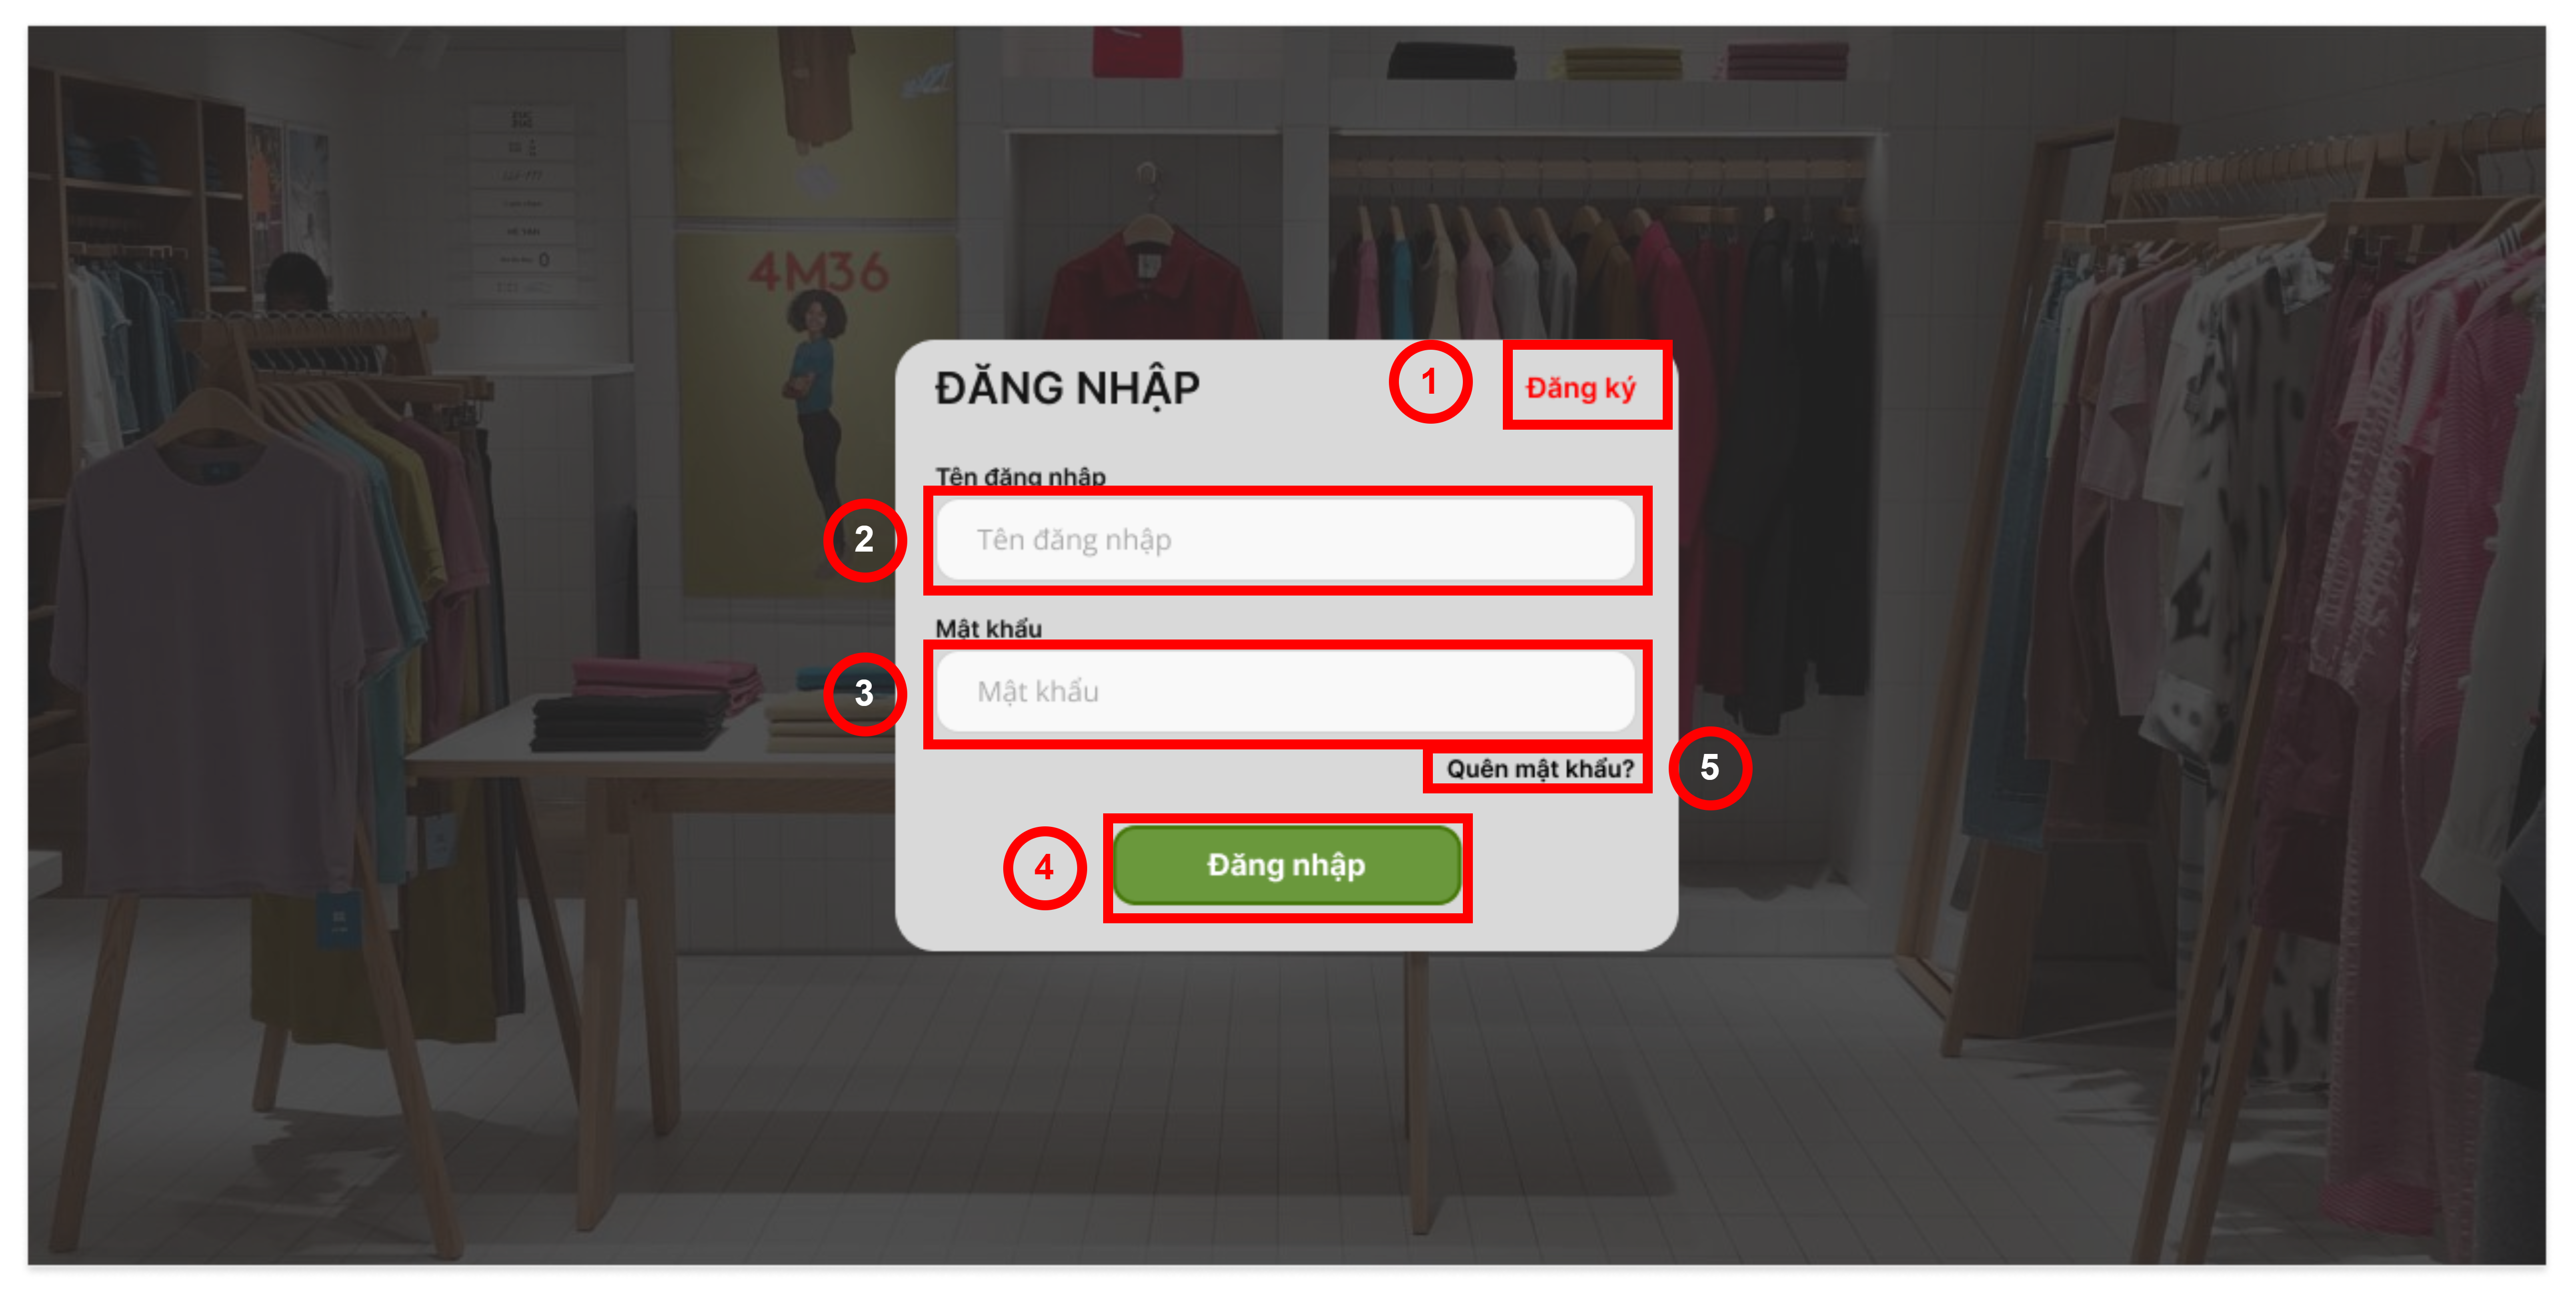
\includegraphics[width=5in]{img/UI/customer/login.png}
        \label{1}
        \newline
        \caption{Giao diện đăng nhập}
    \end{figure}
    \textbf{Mô tả:} 
    \begin{quote}
        \begin{enumerate}
            \item Chọn để chuyển tới trang đăng ký tài khoản.
            \item Nhập tên đăng nhập của tài khoản, yêu cầu tối thiểu 1 ký tự.
            \item Nhập mật khẩu của tài khoản, yêu cầu mật khẩu tối thiếu 6 ký tự.
            \item Chọn để thực hiện đăng nhập tài khoản, nếu thông tin tài khoản đúng thì sẽ được đưa đến giao diện mặc định cho tài khoản.
            \item Chọn "Quên mật khẩu" khi không nhớ mật khẩu của tài khoản để chuyển trang sang trang lấy lại mật khẩu.
        \end{enumerate}        
    \end{quote}

\subsection{Giao diện người dùng}
    \subsubsection{Đăng ký}
    \begin{figure}[!htp]
        \centering
        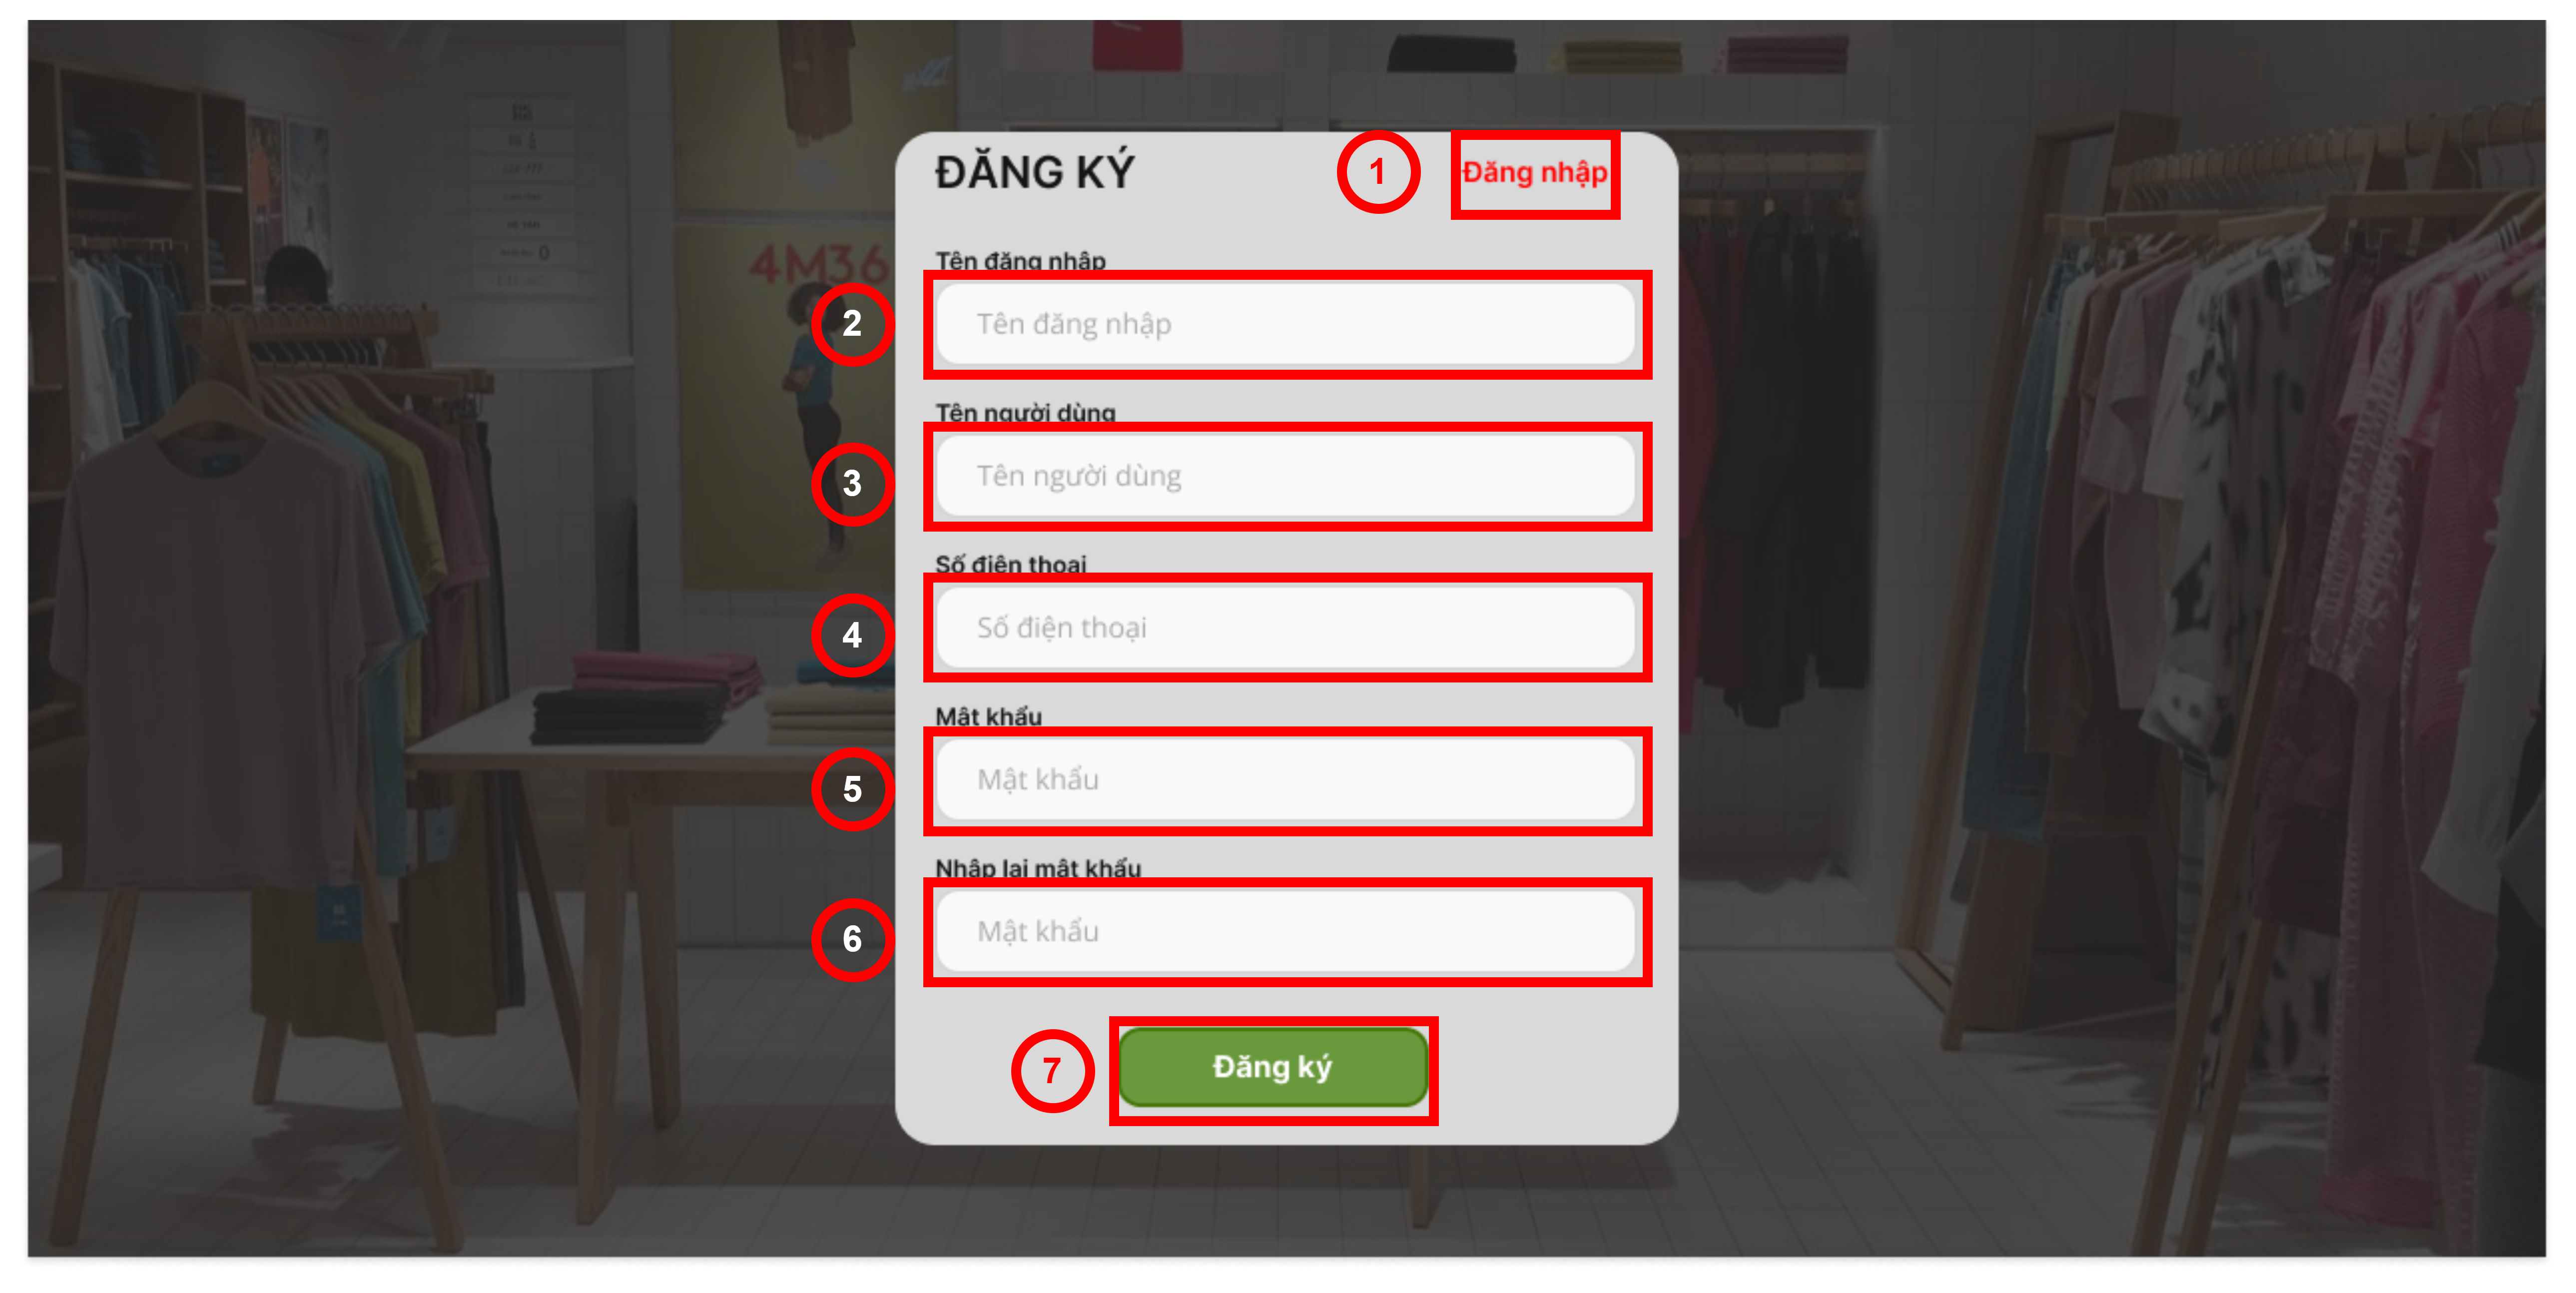
\includegraphics[width=5in]{img/UI/customer/register.png}
        \label{2}
        \newline
        \caption{Giao diện đăng ký tài khoản người dùng}
    \end{figure}
    \textbf{Mô tả:}  
    \begin{quote}
        \begin{enumerate}
            \item Chọn để chuyển tới trang đăng đăng nhập.
            \item Nhập tên đăng nhập của tài khoản, yêu cầu tối thiểu một ký tự.
            \item Nhập tên của người dùng, yêu cầu tối thiểu một ký tự.
            \item Nhập số điện thoại của người dùng, yêu cầu đúng định dạng số điện thoại 10 chữ số, bắt đầu bằng số 09 / 03 / 05 / 07 / 08.
            \item Nhập mật khẩu của tài khoản, yêu cầu tối thiểu 6 ký tự.
            \item Nhập lại mật khẩu của tài khoản, yêu cầu phải giống mật khẩu của tài khoản đã nhập.
            \item Chọn để thực hiện đăng ký tài khoản, nếu đăng ký thành công thì chuyển tới trang đăng nhập.
        \end{enumerate}
    \end{quote}
    
    
    \subsubsection{Tạo lại mật khẩu}
    \begin{figure}[!htp]
        \centering
        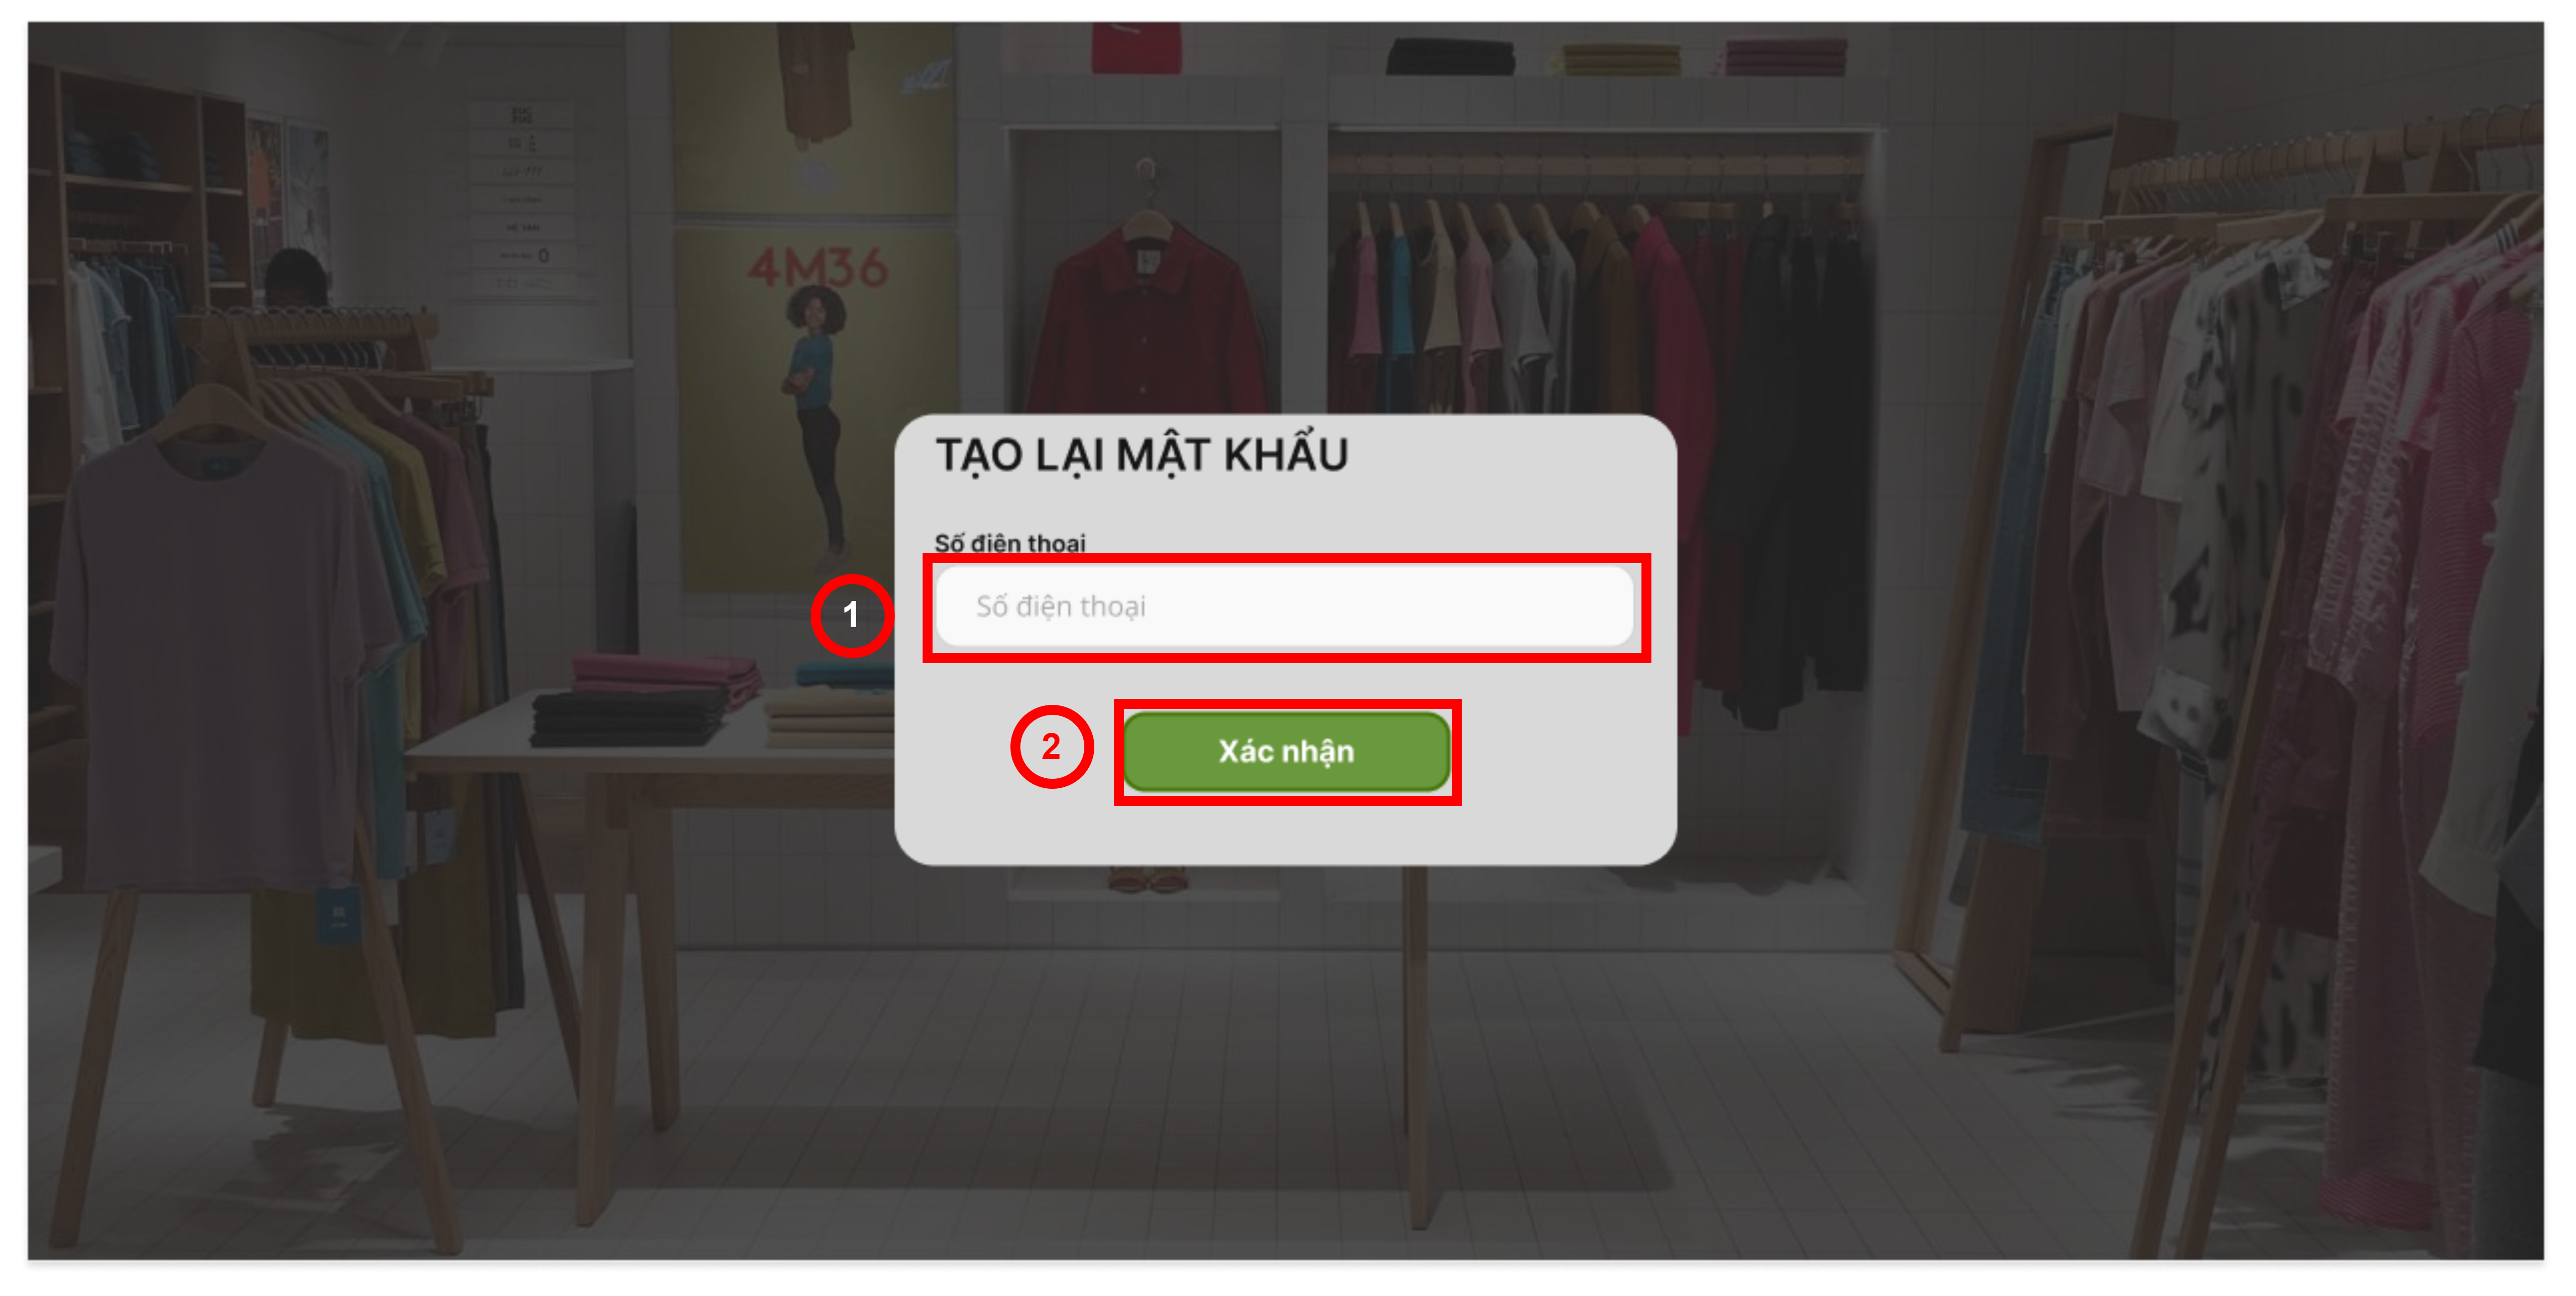
\includegraphics[width=5in]{img/UI/customer/reset_new_password.png}
        \label{3}
        \newline
        \caption{Giao diện tạo lại mật khẩu người dùng}
    \end{figure}
    \textbf{Mô tả:}
    \begin{quote}
        \begin{enumerate}
            \item Người dùng nhập số điện thoại của tài khoản, yêu cầu đúng định dạng số điện thoại 10 chữ số, bắt đầu bằng số 09 / 03 / 05 / 07 / 08.
            \item Người dùng chọn để hệ thống gửi xác nhận tin nhắn OTP và chuyển tới trang xác nhận OTP.
        \end{enumerate}
    \end{quote}
    \begin{figure}[!htp]
        \centering
        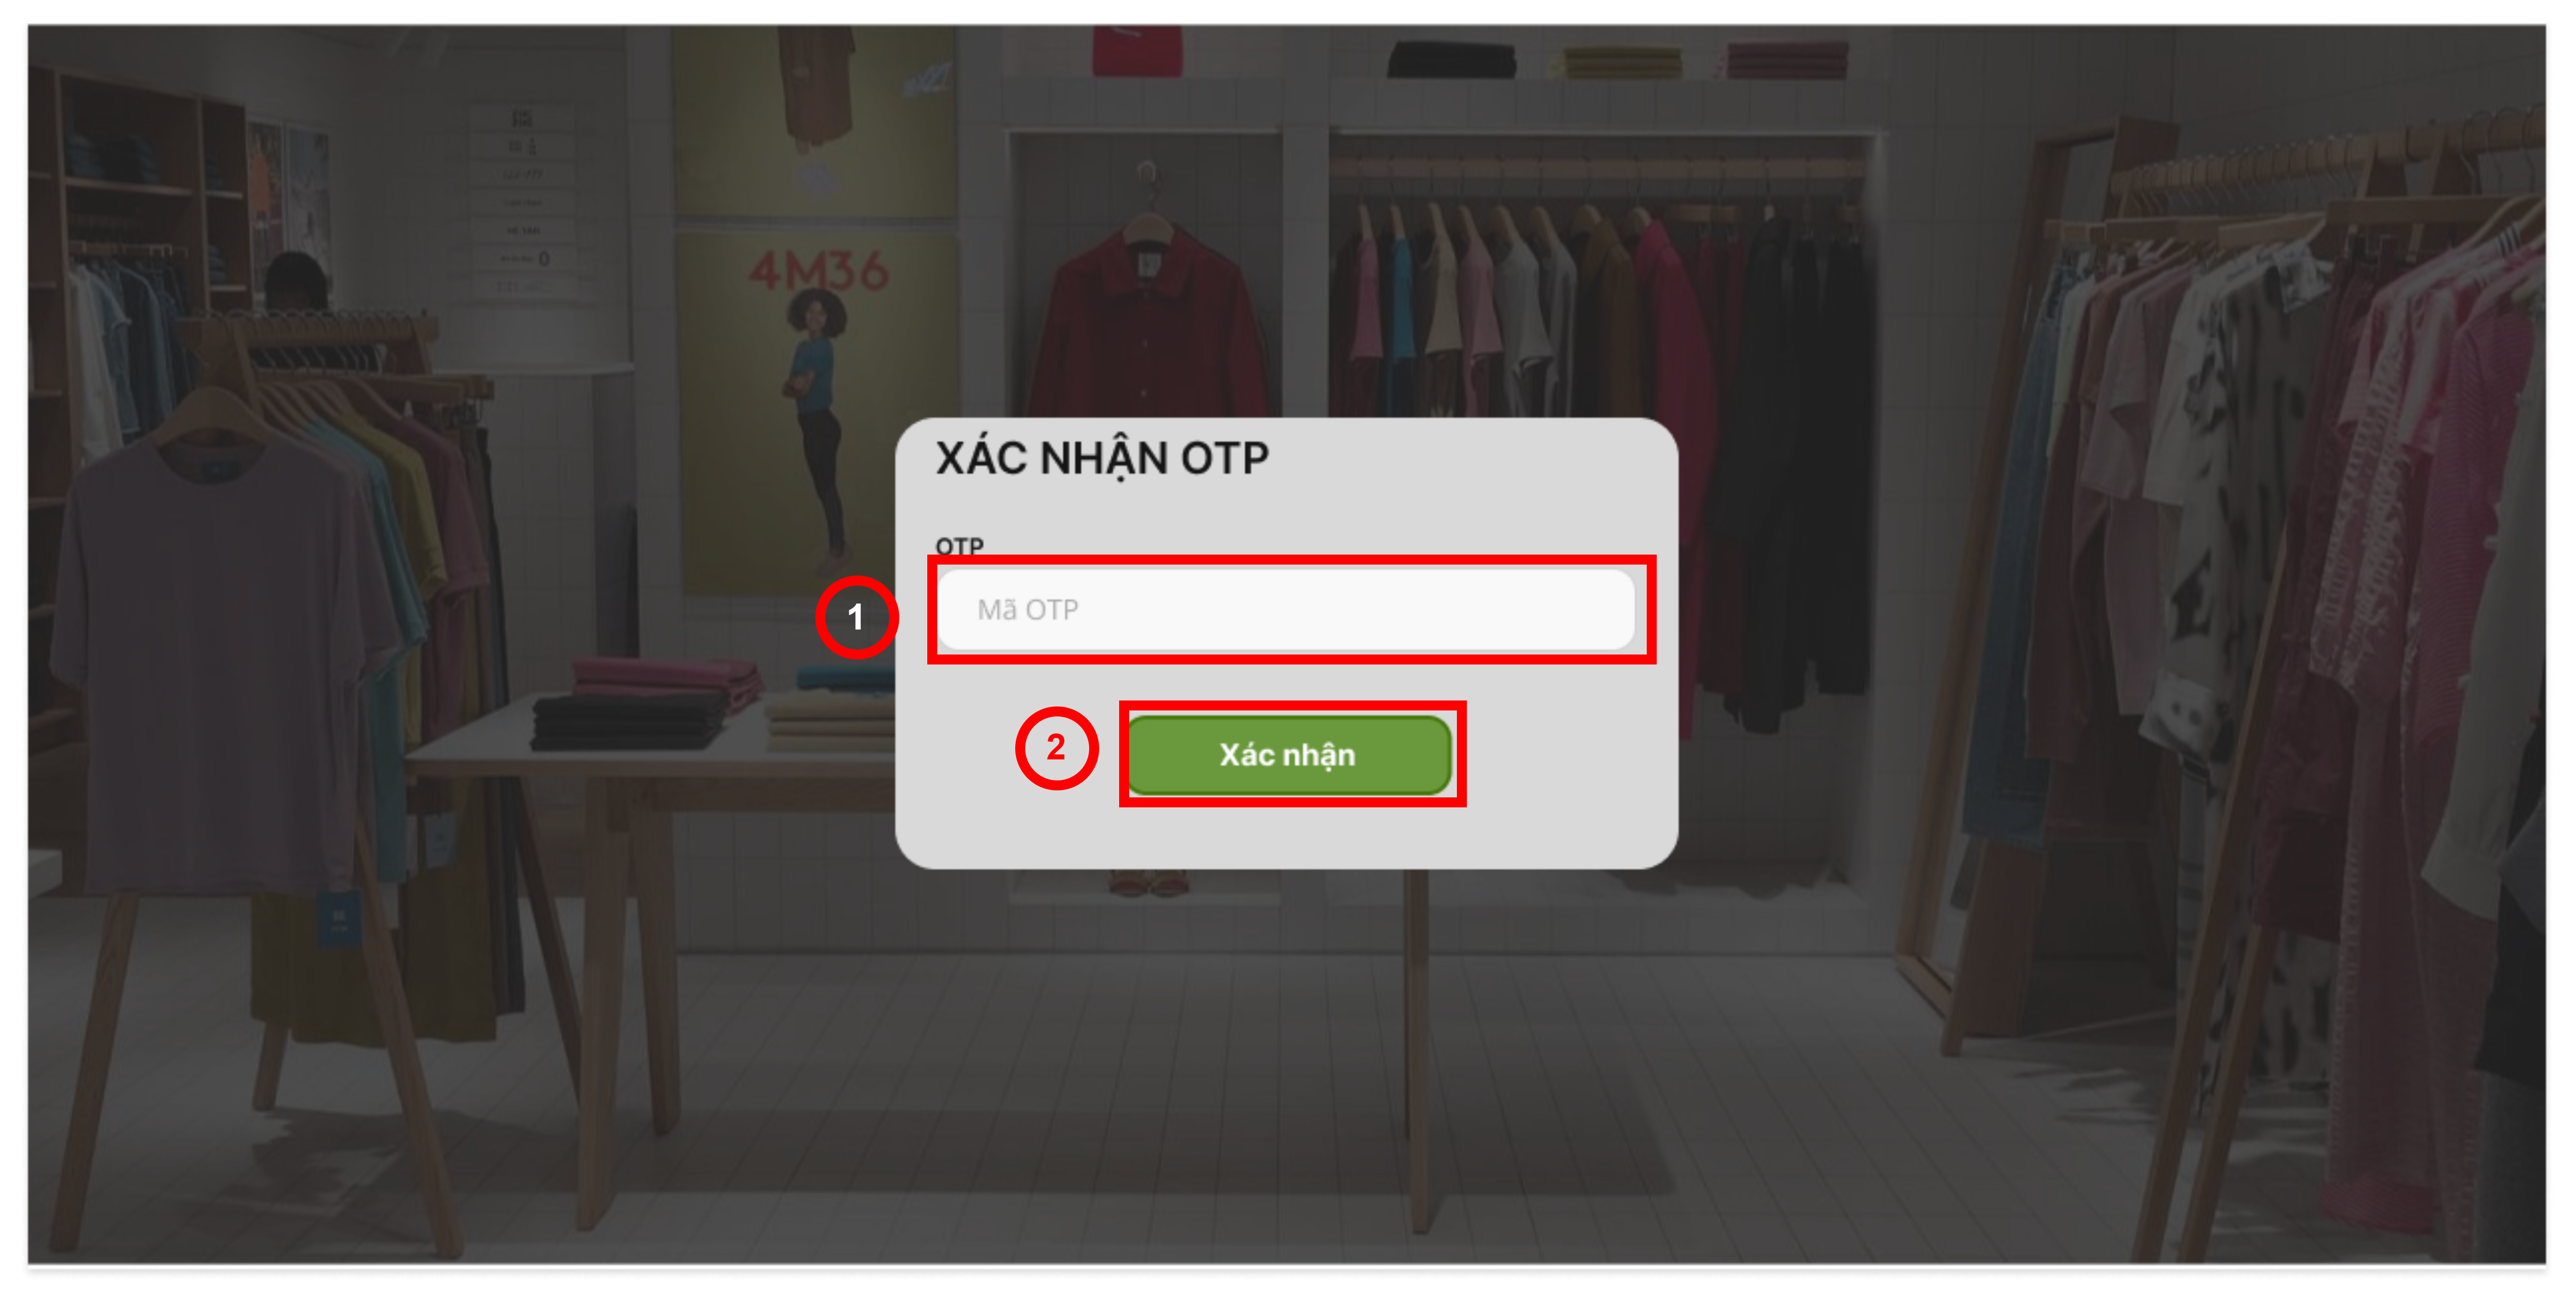
\includegraphics[width=5in]{img/UI/customer/confirm_otp.png}
        \label{4}
        \newline
        \caption{Giao diện xác nhận OTP}
    \end{figure}
    \textbf{Mô tả:}
    \begin{quote}
        \begin{enumerate}
            \item Người dùng nhập OTP đã được gửi qua tin nhắn, yêu cầu 6 ký tự.
            \item Người dùng chọn để hệ thống xác nhận và thông tin hợp lệ sẽ được chuyển đến trang tạo lại mật khẩu mới.
        \end{enumerate}
    \end{quote}
    \textbf{Mô tả:}
    \begin{quote}
        \begin{enumerate}
            \item Người dùng nhập số điện thoại của tài khoản, yêu cầu đúng định dạng số điện thoại 10 chữ số, bắt đầu bằng số 09 / 03 / 05 / 07 / 08.
            \item Người dùng chọn để hệ thống gửi xác nhận tin nhắn OTP và chuyển tới trang xác nhận OTP.
        \end{enumerate}
    \end{quote}
    \begin{figure}[!htp]
        \centering
        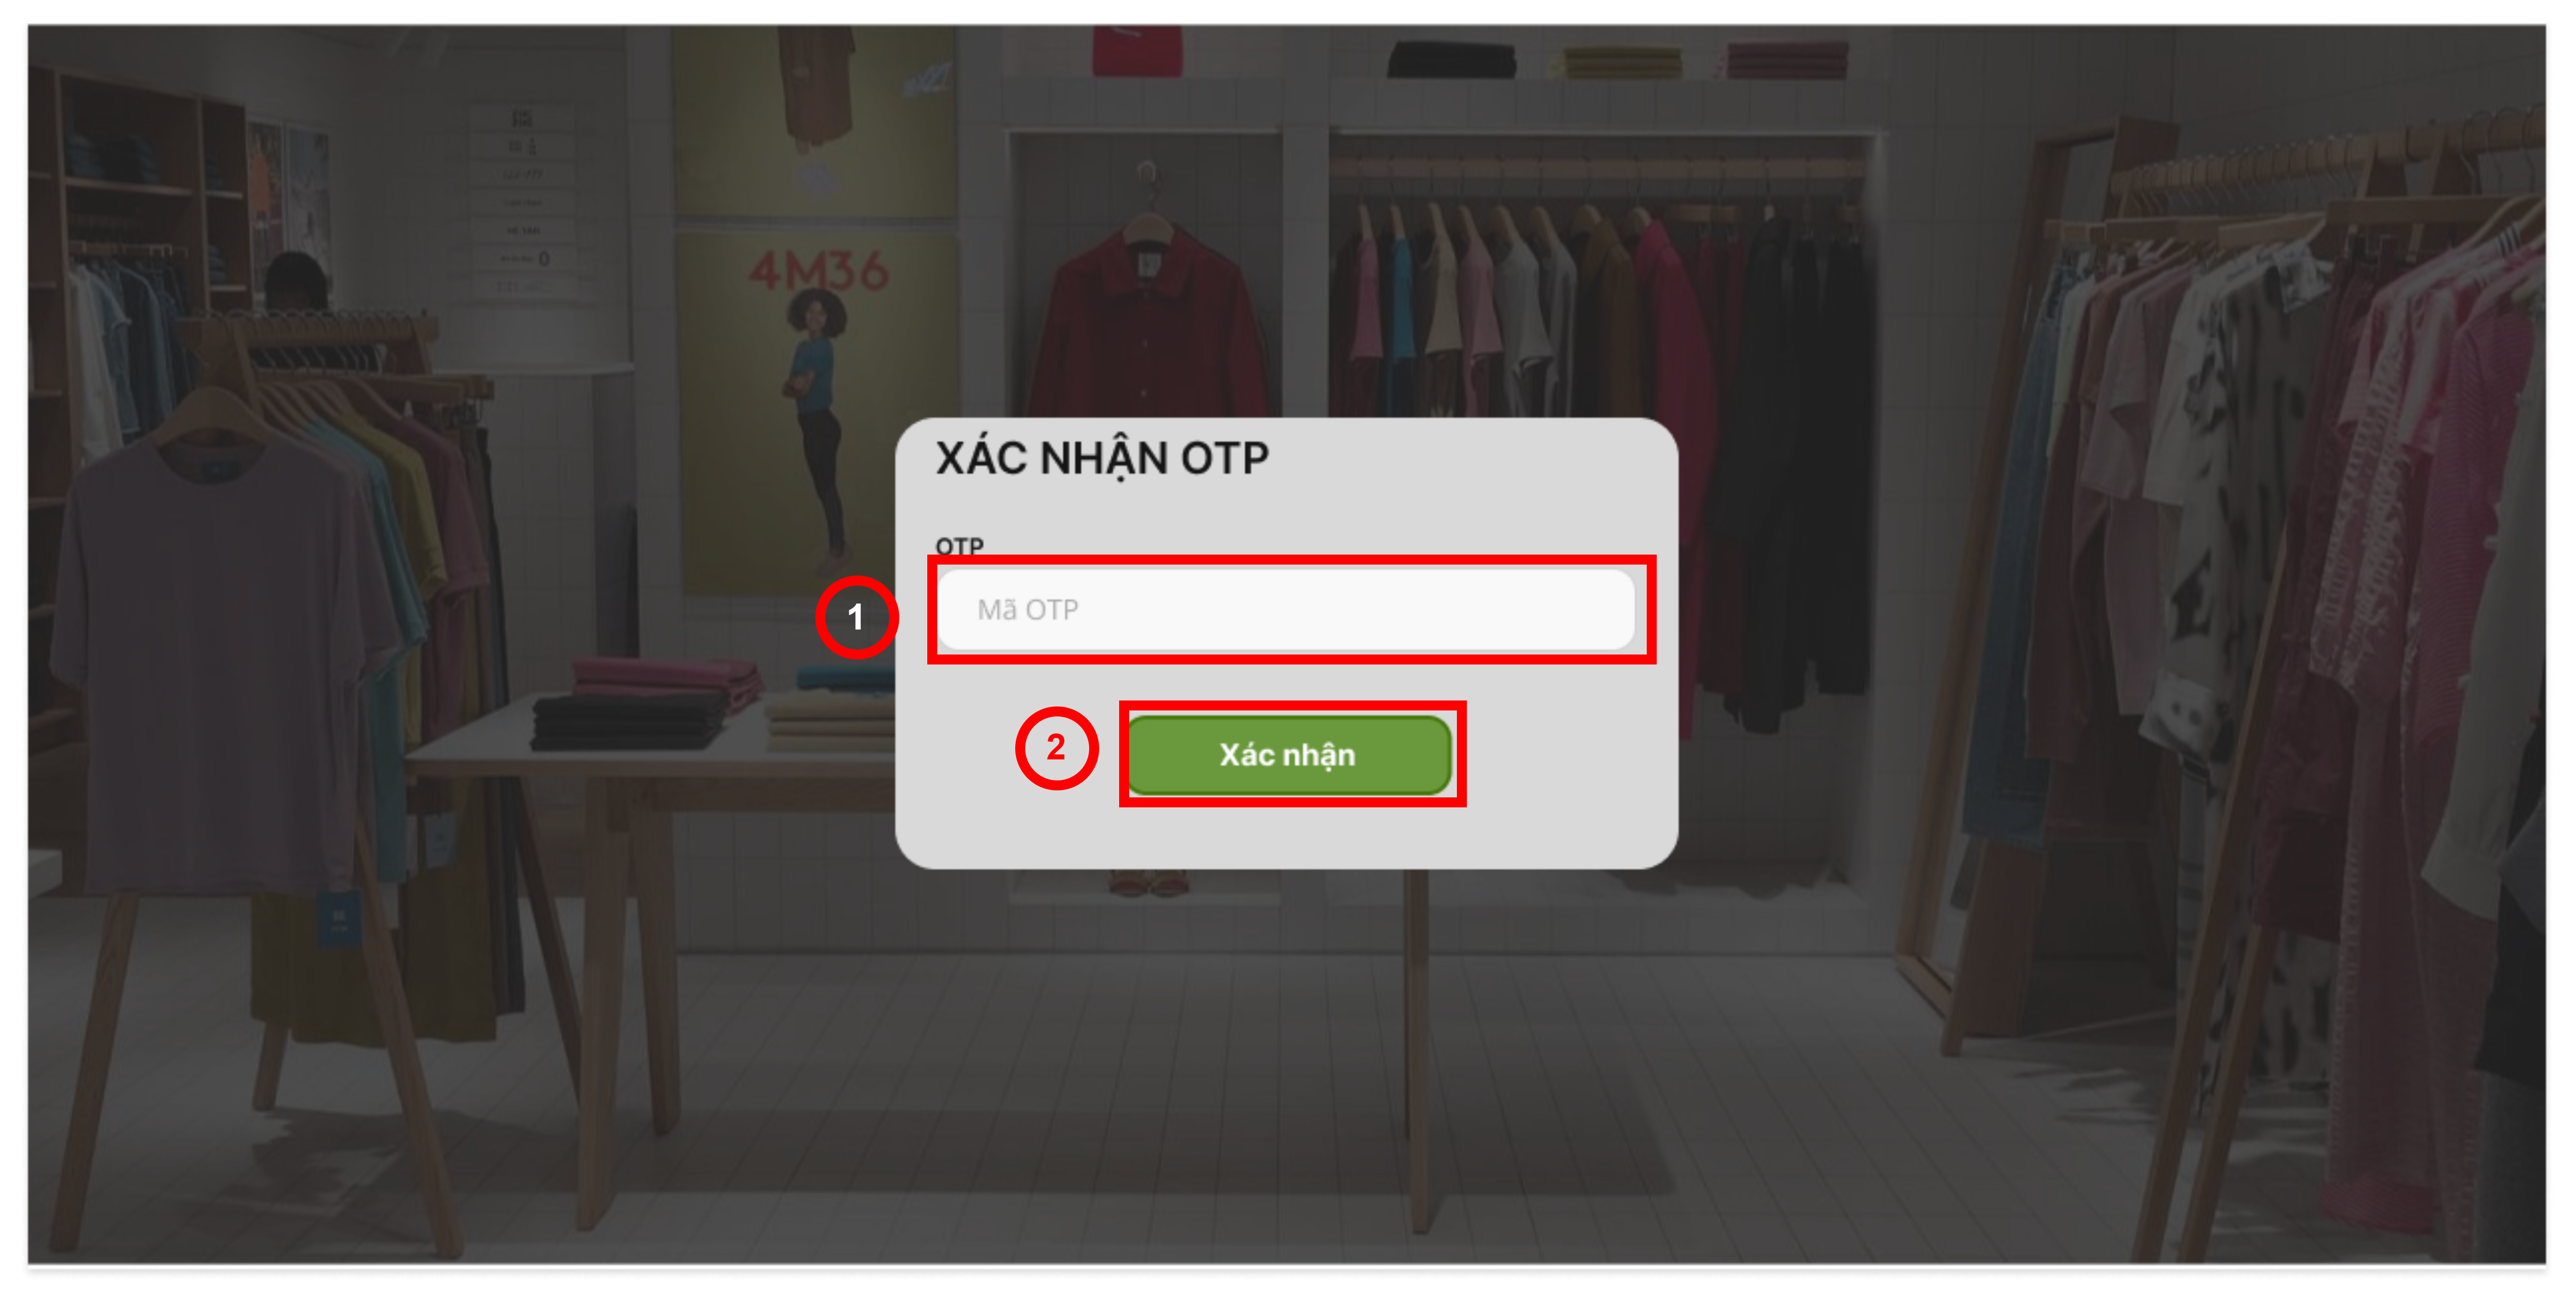
\includegraphics[width=5in]{img/UI/customer/confirm_otp.png}
        \label{5}
        \newline
        \caption{Giao diện tạo lại mật khẩu mới}
    \end{figure}
    \textbf{Mô tả:}
    \begin{quote}
        \begin{enumerate}
            \item Người dùng nhập mật khẩu mới cho tài khoản, yêu cầu tối thiểu 6 ký tự.
            \item Người dùng nhập lại mật khẩu mới cho tài khoản, yêu cầu phải giống với mật khẩu mới.
            \item Người dùng chọn "Xác nhận" để cập nhật lại mật khẩu mới cho tài khoản.
        \end{enumerate}
    \end{quote}
    
    \subsubsection{Header}
    \begin{figure}[!htp]
        \centering
        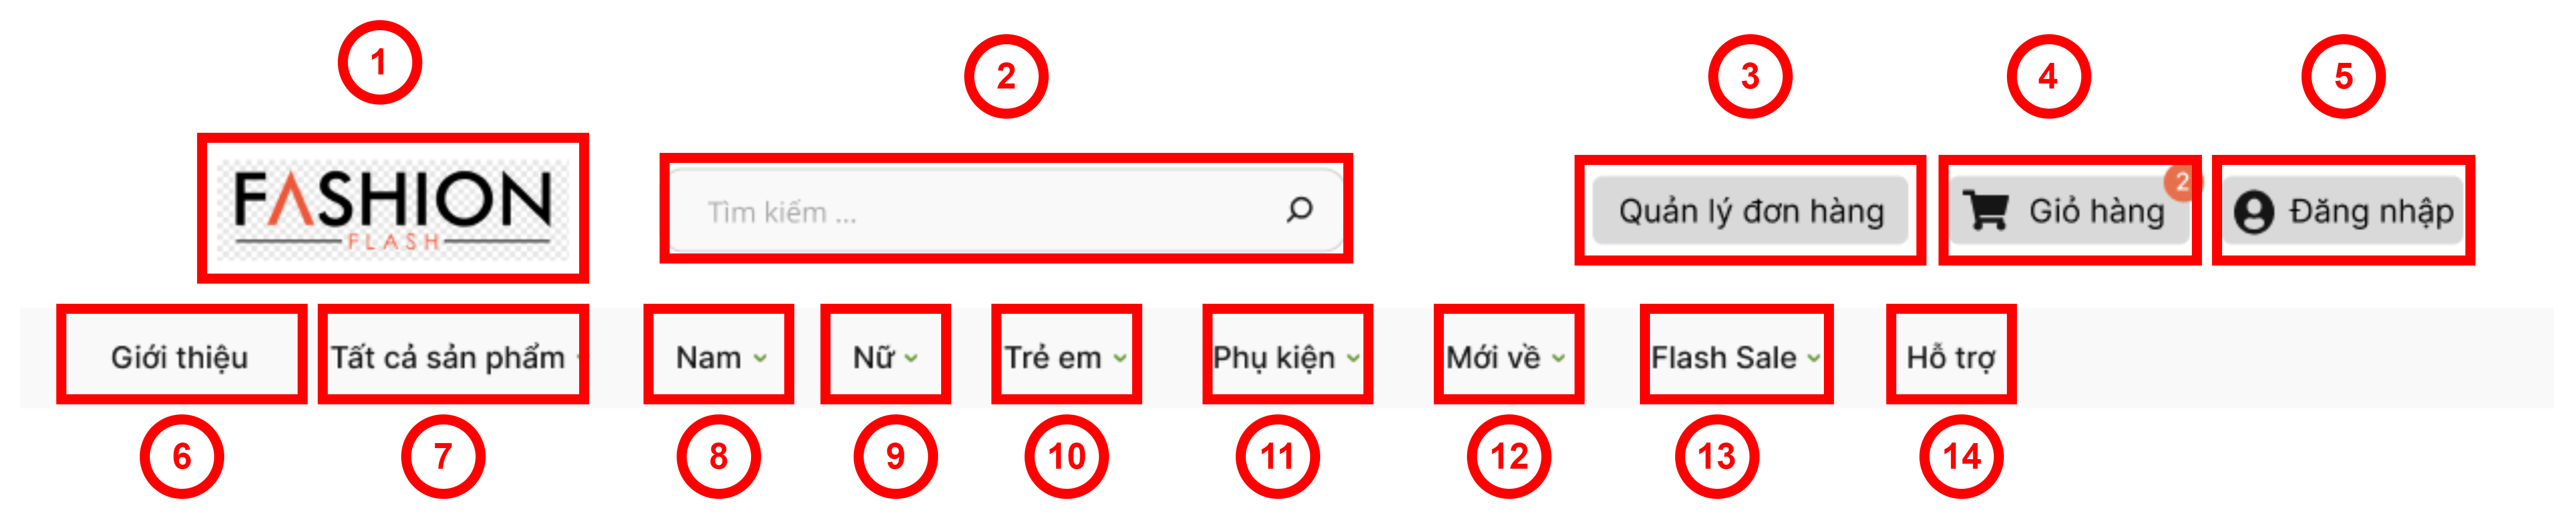
\includegraphics[width=5in]{img/UI/customer/header.png}
        \label{6}
        \newline
        \caption{Giao diện phần header}
    \end{figure}
    \textbf{Mô tả:}  
    \begin{quote}
        \begin{enumerate}
            \item Chọn để chuyển tới trang chủ.
            \item Nhập tên sản phẩm cần tìm và nhấn enter để tìm kiếm sản phẩm.
            \item Chọn để chuyển đến trang quản lý lịch sử đơn hàng đã thực hiện.
            \item Chọn để chuyển đến trang quản lý giỏ hàng.
            \item Chọn để đăng nhập.
            \item Chọn để chuyển đến trang giới thiệu về hệ thống cửa hàng.
            \item Chọn để truyển đến trang tất cả sản phẩm.
            \item Chọn để truyển đến trang tất cả sản phẩm với lựa chọn lọc sẵn là sản phẩm dành cho nam.
            \item Chọn để truyển đến trang tất cả sản phẩm với lựa chọn lọc sẵn là sản phẩm dành cho nữ.
            \item Chọn để truyển đến trang tất cả sản phẩm với lựa chọn lọc sẵn là sản phẩm dành cho trẻ em.
            \item Chọn để truyển đến trang tất cả sản phẩm với lựa chọn lọc sẵn là sản phẩm thuộc dòng phụ kiện.
            \item Chọn để truyển đến trang các sản phẩm mới về.
            \item Chọn để truyển đến trang các sản phẩm đang được flash sale.
            \item Chọn để truyển đến trang hỗ trợ cho khách hàng.
        \end{enumerate}
    \end{quote}
    
    \subsubsection{Footer}
    \begin{figure}[!htp]
        \centering
        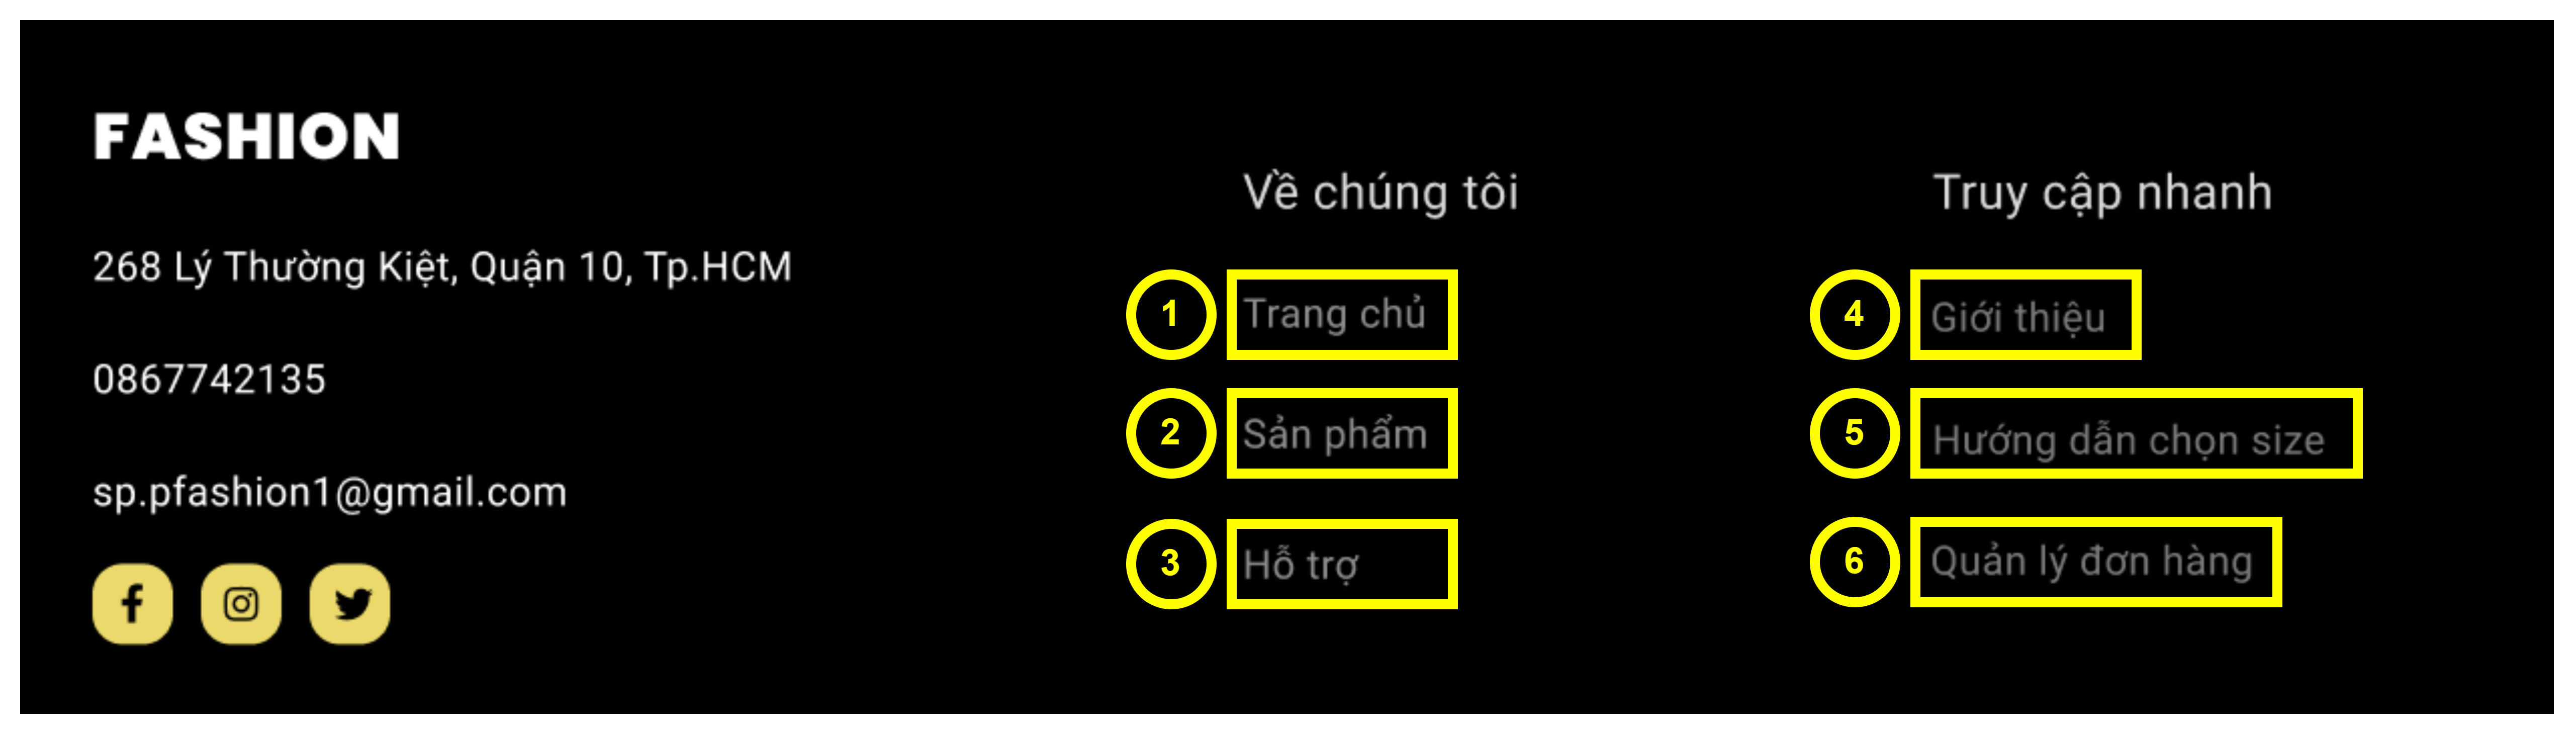
\includegraphics[width=5in]{img/UI/customer/footer.png}
        \label{7}
        \newline
        \caption{Giao diện phần footer}
    \end{figure}
    \textbf{Mô tả:}  
    \begin{quote}
        \begin{enumerate}
            \item Chọn để chuyển tới trang chủ.
            \item Chọn để truyển đến trang tất cả sản phẩm.
            \item Chọn để truyển đến trang hỗ trợ cho khách hàng.
            \item Chọn để chuyển đến trang giới thiệu về hệ thống cửa hàng.
            \item Chọn để xem hướng dẫn chọn size.
            \item Chọn để chuyển đến trang quản lý lịch sử đơn hàng đã thực hiện.
        \end{enumerate}
    \end{quote}
    
    \newpage
    \subsubsection{Trang chủ}
    \begin{figure}[!htp]
        \centering
        \includegraphics[width=3.5in]{img/UI/customer/home.png}
        \label{8}
        \newline
        \caption{Giao diện trang chủ khi người dùng truy cập vào trang web}
    \end{figure}
    \textbf{Mô tả:}  
    \begin{quote}
        \begin{enumerate}
            \item Chọn để xem thông tin chi tiết của sản phẩm.
            \item Chọn để thêm nhanh sản phẩm vào giỏ hàng.
        \end{enumerate}
    \end{quote}    
    
    \subsubsection{Thông tin chi tiết sản phẩm}
    \begin{figure}[!htp]
        \centering
        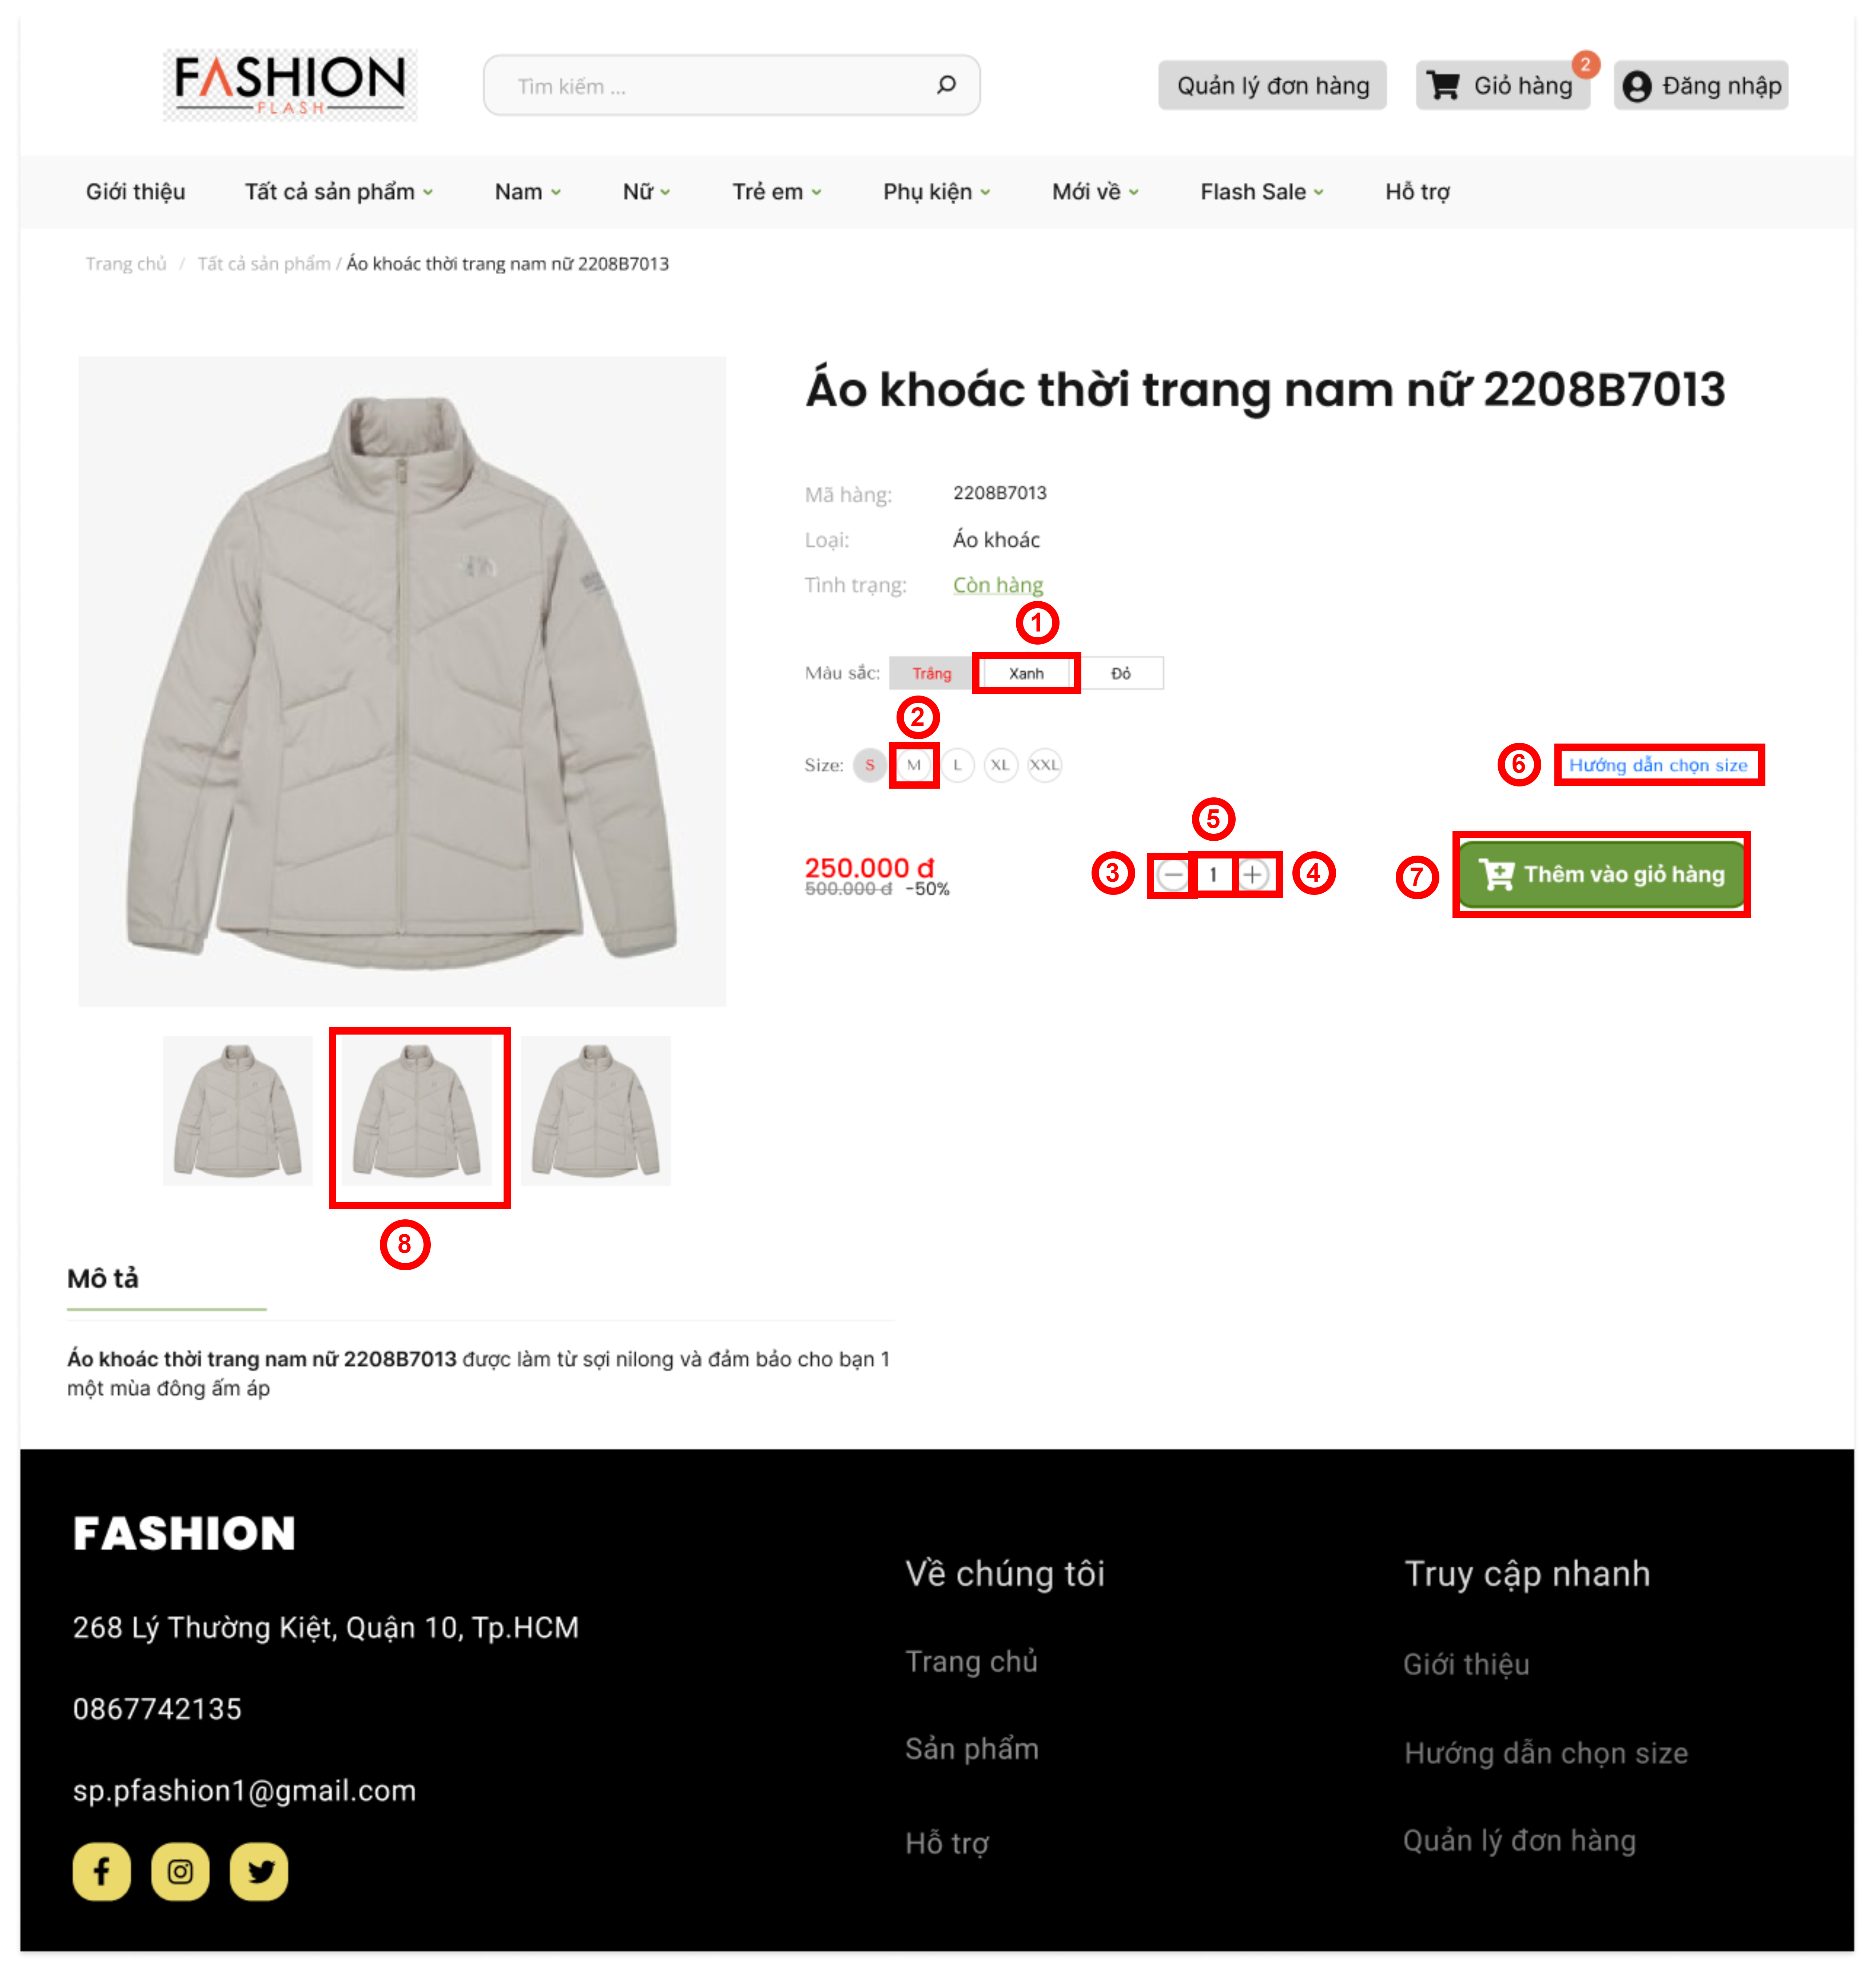
\includegraphics[width=5in]{img/UI/customer/product_detail.png}
        \label{9}
        \newline
        \caption{Giao diện thông tin chi tiết của sản phẩm}
    \end{figure}
    \textbf{Mô tả:}  
    \begin{quote}
        \begin{enumerate}
            \item Chọn màu của sản phẩm mà người dùng muốn.
            \item Chọn size của sản phẩm mà người dùng muốn.
            \item Chọn để giảm số lượng mà người dùng muốn.
            \item Chọn để tăng số lượng mà người dùng muốn.
            \item Nhập để thay đổi số lượng mà người dùng muốn.
            \item Chọn để xem hướng dẫn chọn size cho sản phẩm.
            \item Chọn để thêm sản phẩm với màu sắc, size và số lượng mà người dùng đã chọn.
            \item Chọn để xem ảnh chi tiết mà người dùng muốn.
        \end{enumerate}
    \end{quote}
    
    \begin{figure}[!htp]
        \centering
        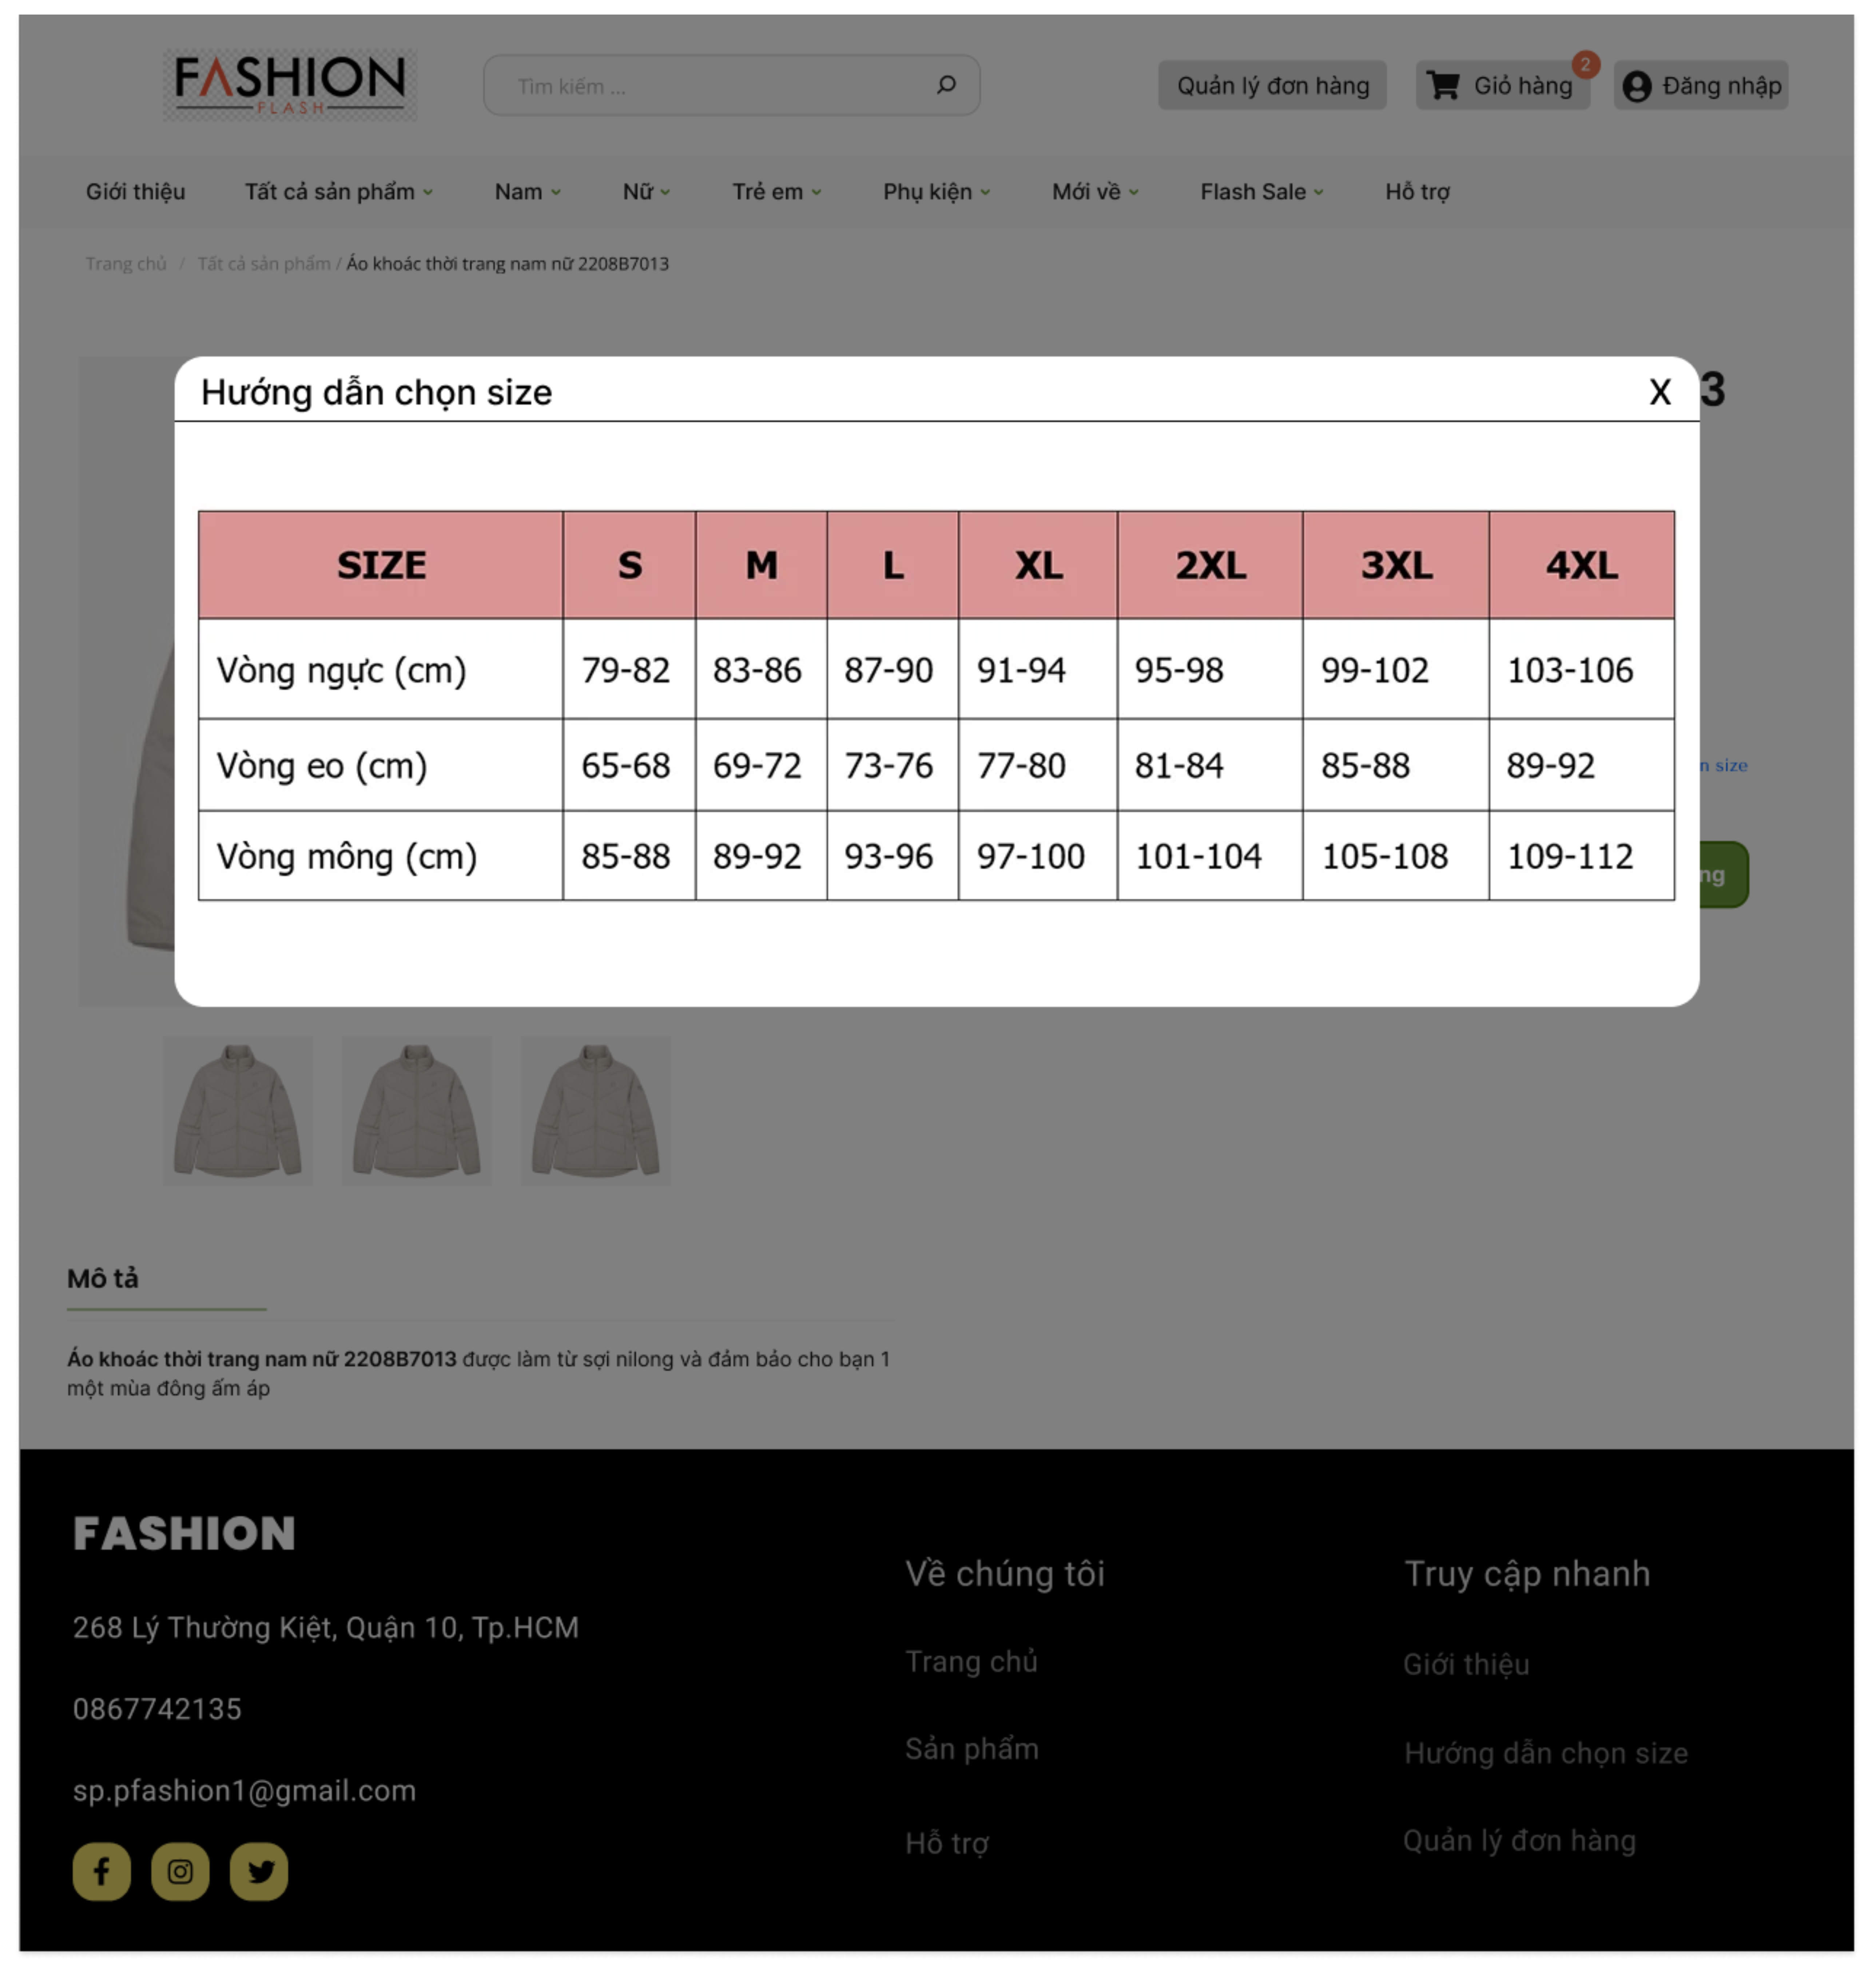
\includegraphics[width=5in]{img/UI/customer/guide_size.png}
        \label{10}
        \newline
        \caption{Giao diện hướng dẫn chọn size cho sản phẩm}
    \end{figure}
    \newpage
    
    \subsubsection{Giỏ hàng}
    \begin{figure}[!htp]
        \centering
        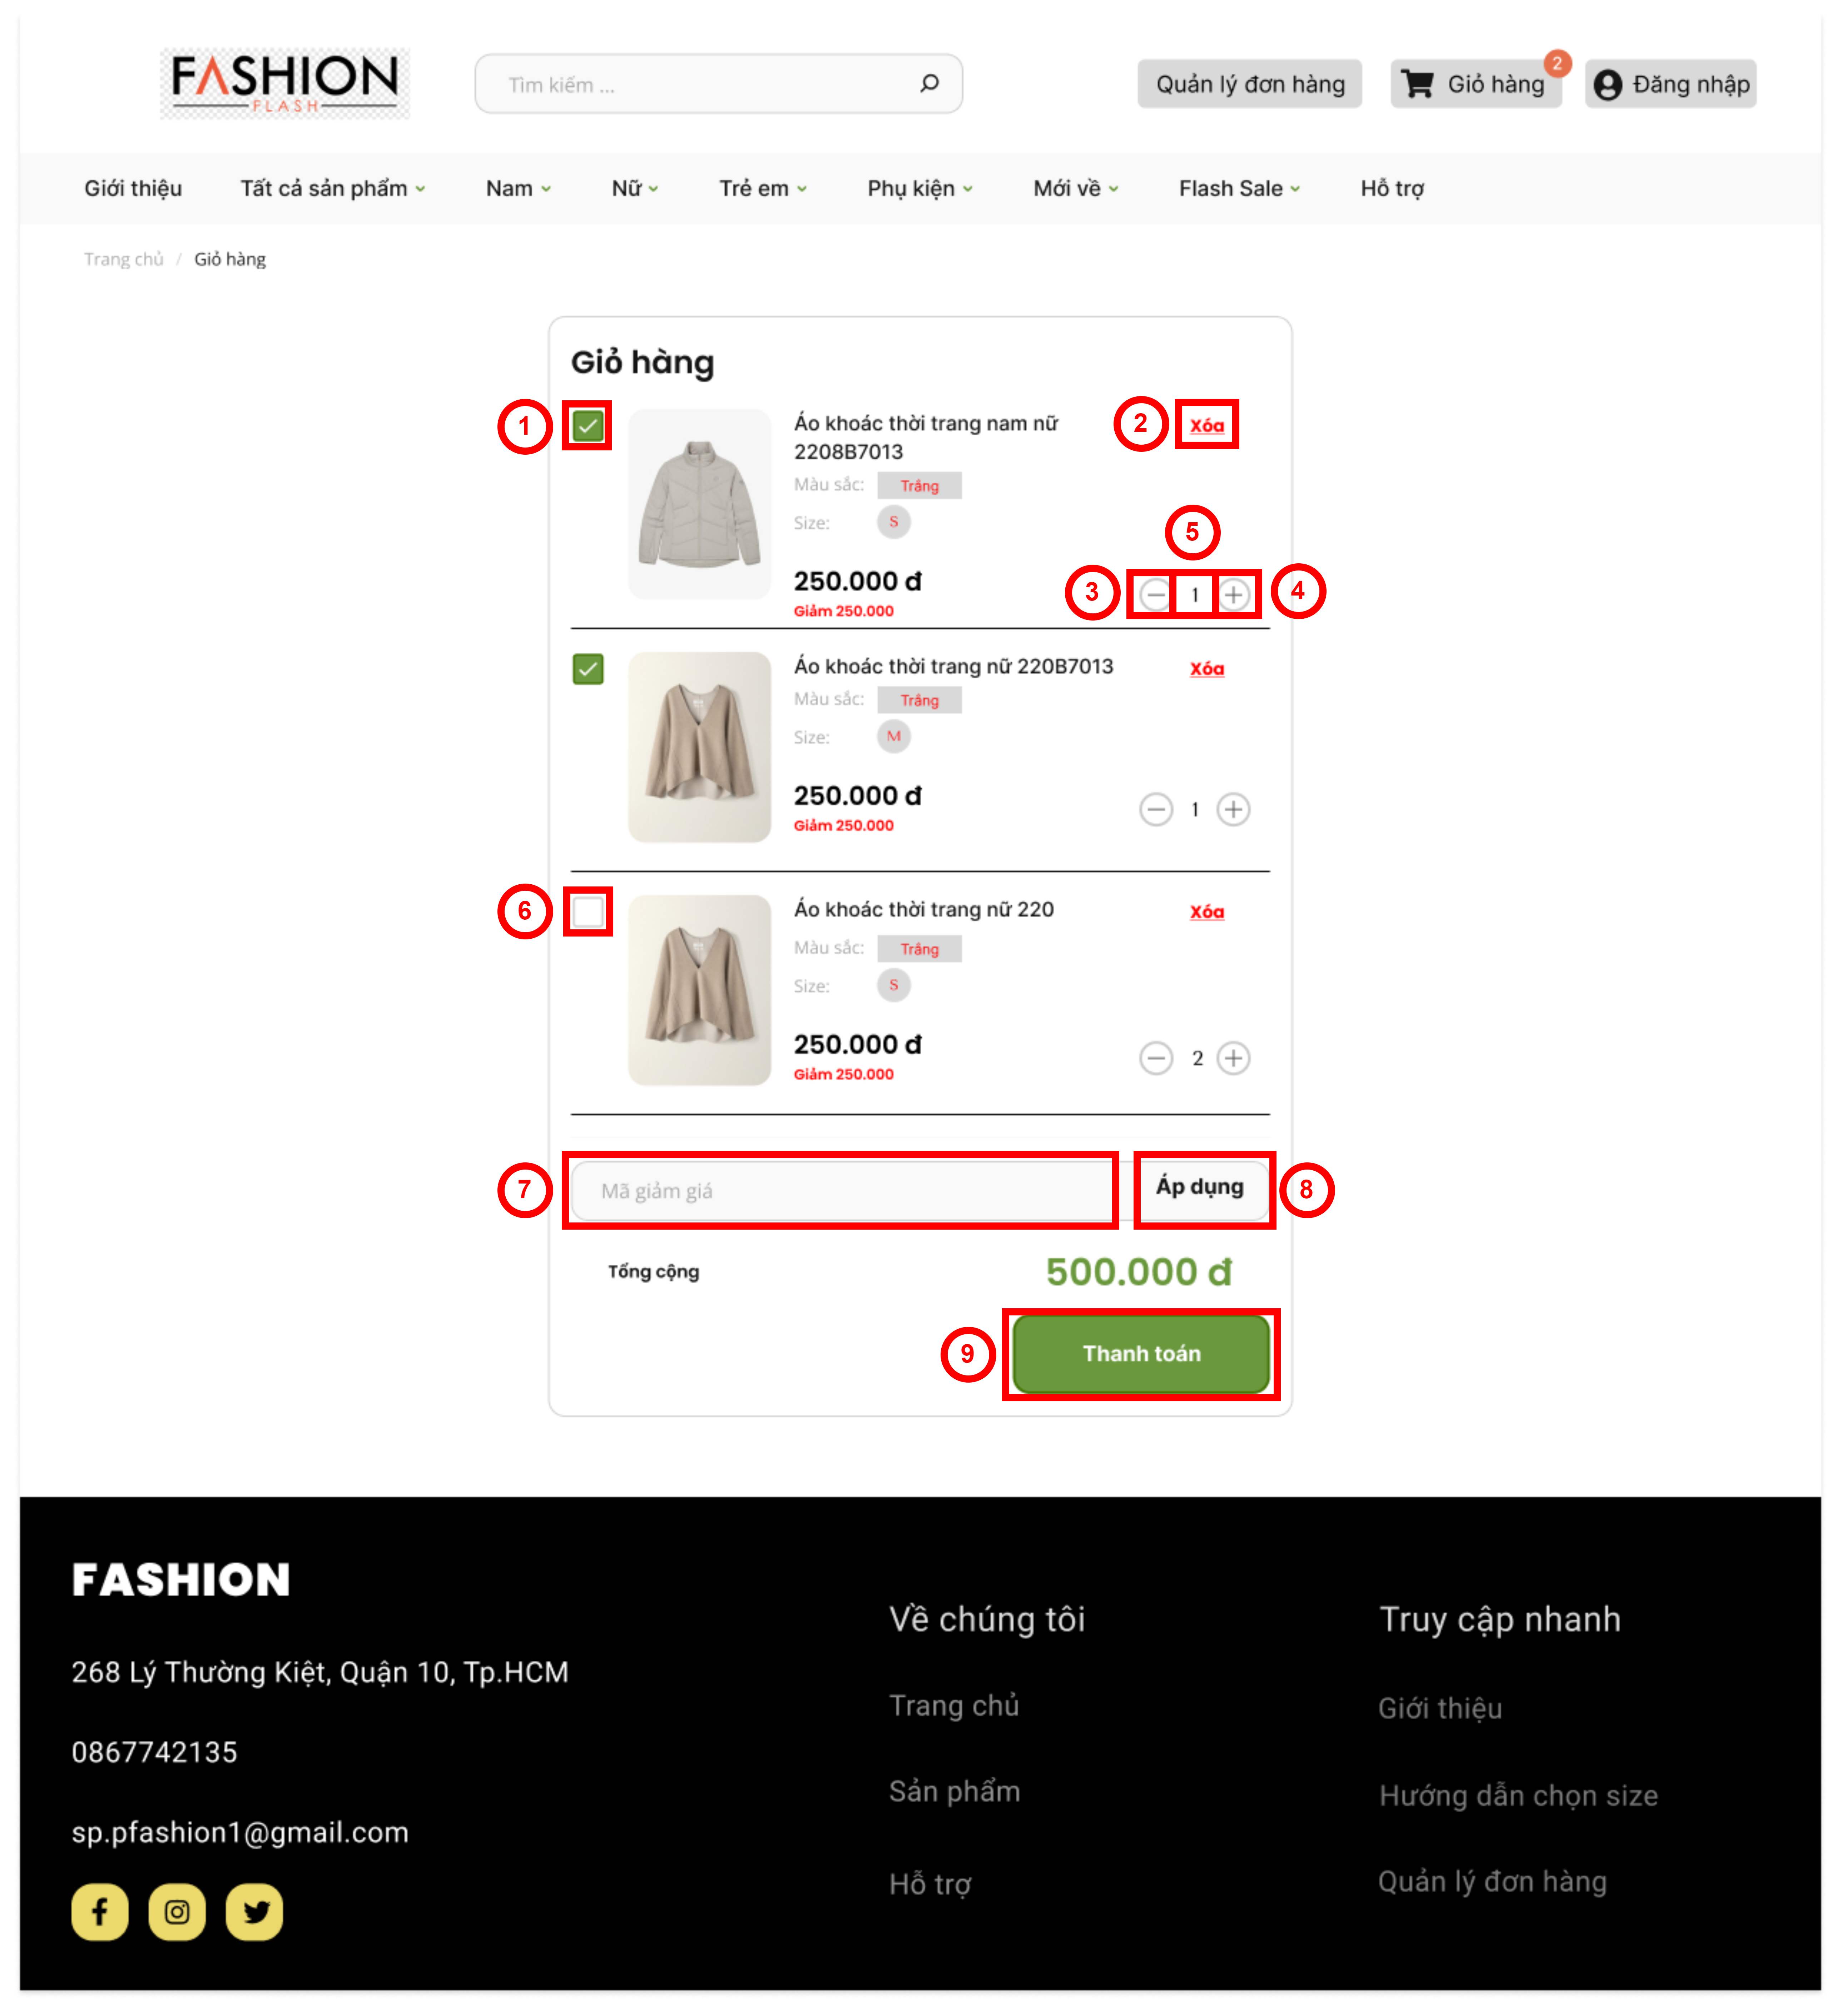
\includegraphics[width=5in]{img/UI/customer/cart.png}
        \label{11}
        \newline
        \caption{Giao diện quản lý giỏ hàng.}
    \end{figure}
    \textbf{Mô tả:}  
    \begin{quote}
        \begin{enumerate}
            \item Chọn để loại sản phẩm khỏi danh sách muốn đặt hàng.
            \item Chọn để xóa sản phẩm khỏi giỏ hàng.
            \item Chọn để giảm số lượng mà người dùng muốn.
            \item Chọn để tăng số lượng mà người dùng muốn.
            \item Nhập để thay đổi số lượng mà người dùng muốn.
            \item Chọn để thêm sản phẩm vào danh sách muốn đặt hàng.
            \item Nhập mã giảm giá.
            \item Chọn để áp dụng mã giảm giá.
            \item Chọn để thực hiện thanh toán để đặt hàng.
        \end{enumerate}
    \end{quote}   
    
    \subsubsection{Thanh toán}
    \begin{figure}[!htp]
        \centering
        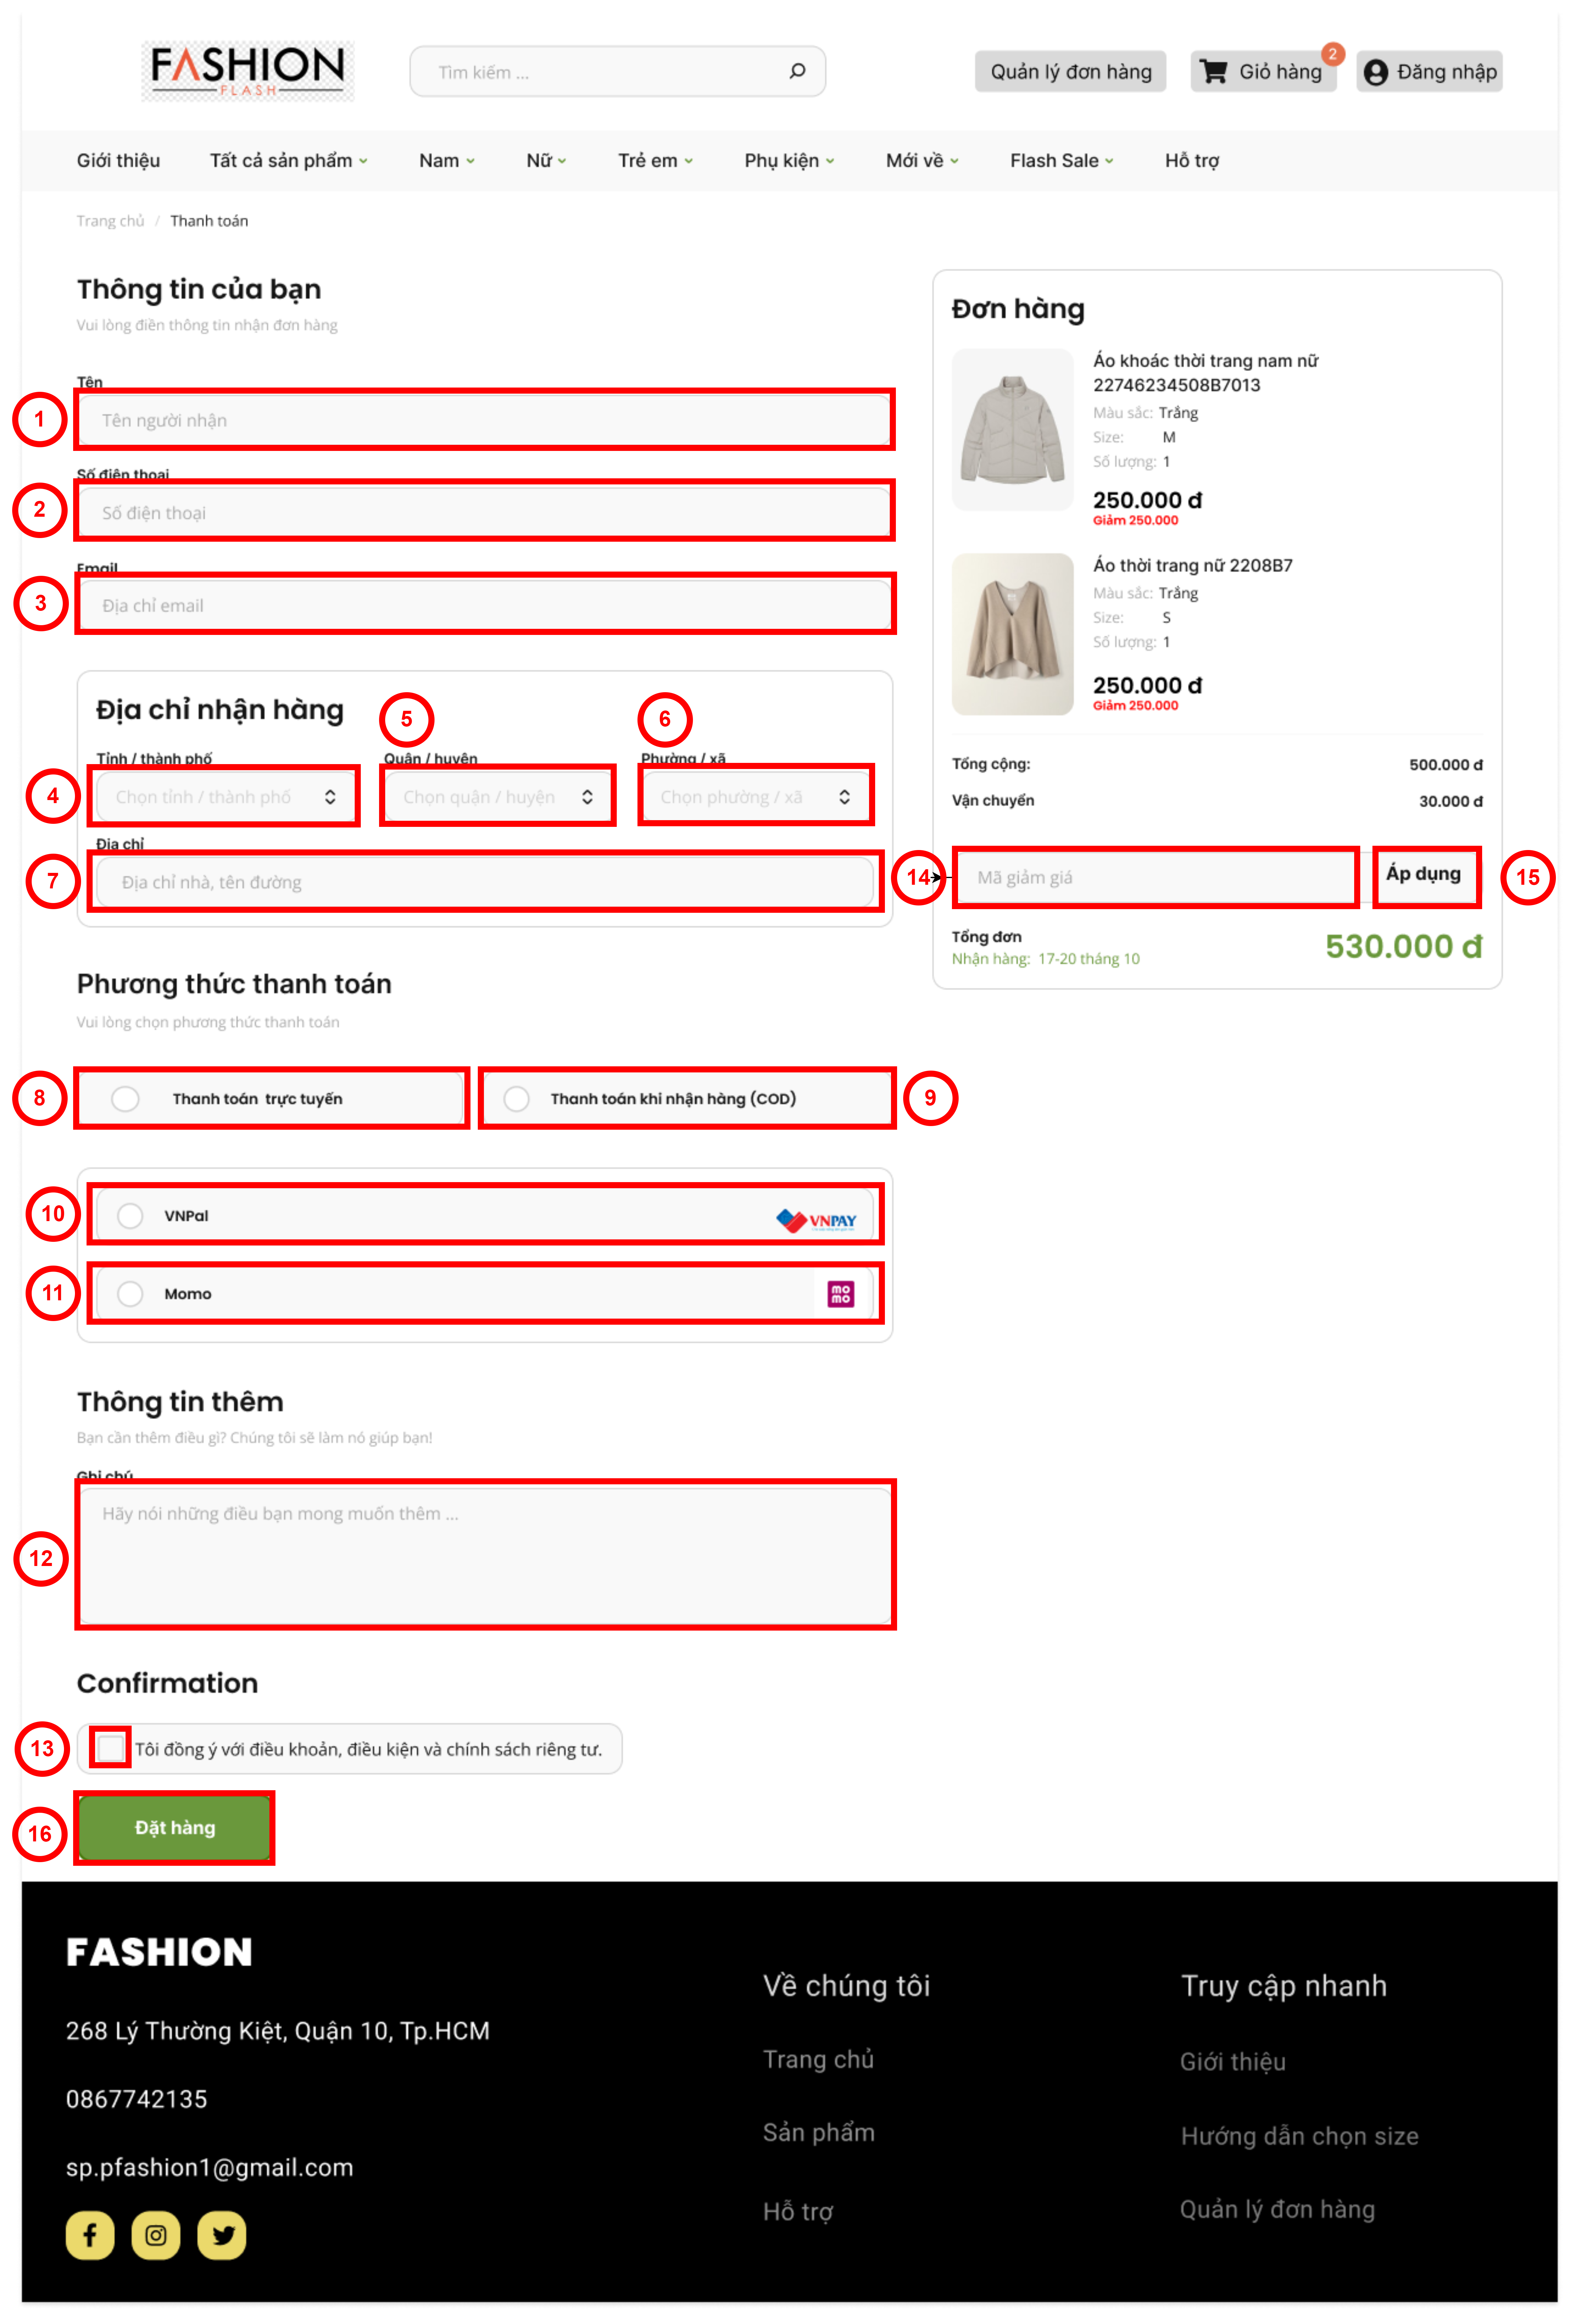
\includegraphics[width=5in]{img/UI/customer/payment.png}
        \label{12}
        \newline
        \caption{Giao diện thanh toán.}
    \end{figure}
    \textbf{Mô tả:}  
    \begin{quote}
        \begin{enumerate}
            \item Nhập tên người nhận hàng.
            \item Nhập số điện thoại người nhận hàng.
            \item Nhập địa chỉ email người nhận hàng.
            \item Nhập địa chỉ tỉnh/thành nhận hàng.
            \item Nhập địa chỉ quận/huyện nhận hàng.
            \item Nhập địa chỉ phường/xã nhận hàng.
            \item Nhập địa chỉ số nhà, tên đường nhận hàng.
            \item Chọn để thực hiện thanh toán trực tuyến.
            \item Chọn để thực hiện thanh toán trực tiếp khi nhận hàng.
            \item Chọn để thực hiện thanh toán trực tuyến thông qua VNPay.
            \item Chọn để thực hiện thanh toán trực tuyến thông qua Momo.
            \item Nhập để thêm ghi chú cho đơn hàng.
            \item Chọn để xác nhận đồng ý điều khoản mua hàng.
            \item Nhập mã giảm giá.
            \item Chọn để kiểm tra mã giảm giá và áp dụng giảm giá vào đơn hàng.
            \item Chọn để xác nhận đặt hàng, nếu chọn thanh toán trực tuyến thì sẽ được chuyển đến trang thanh toán của bên thứ ba mà người dùng chọn, nếu chọn thanh toán khi nhận hàng thì đơn hàng sẽ được hoàn tất khi tất cả thông tin hợp lệ.
        \end{enumerate}
    \end{quote}       
    
    \subsubsection{Giao diện quản lý đơn hàng}
    \begin{figure}[!htp]
        \centering
        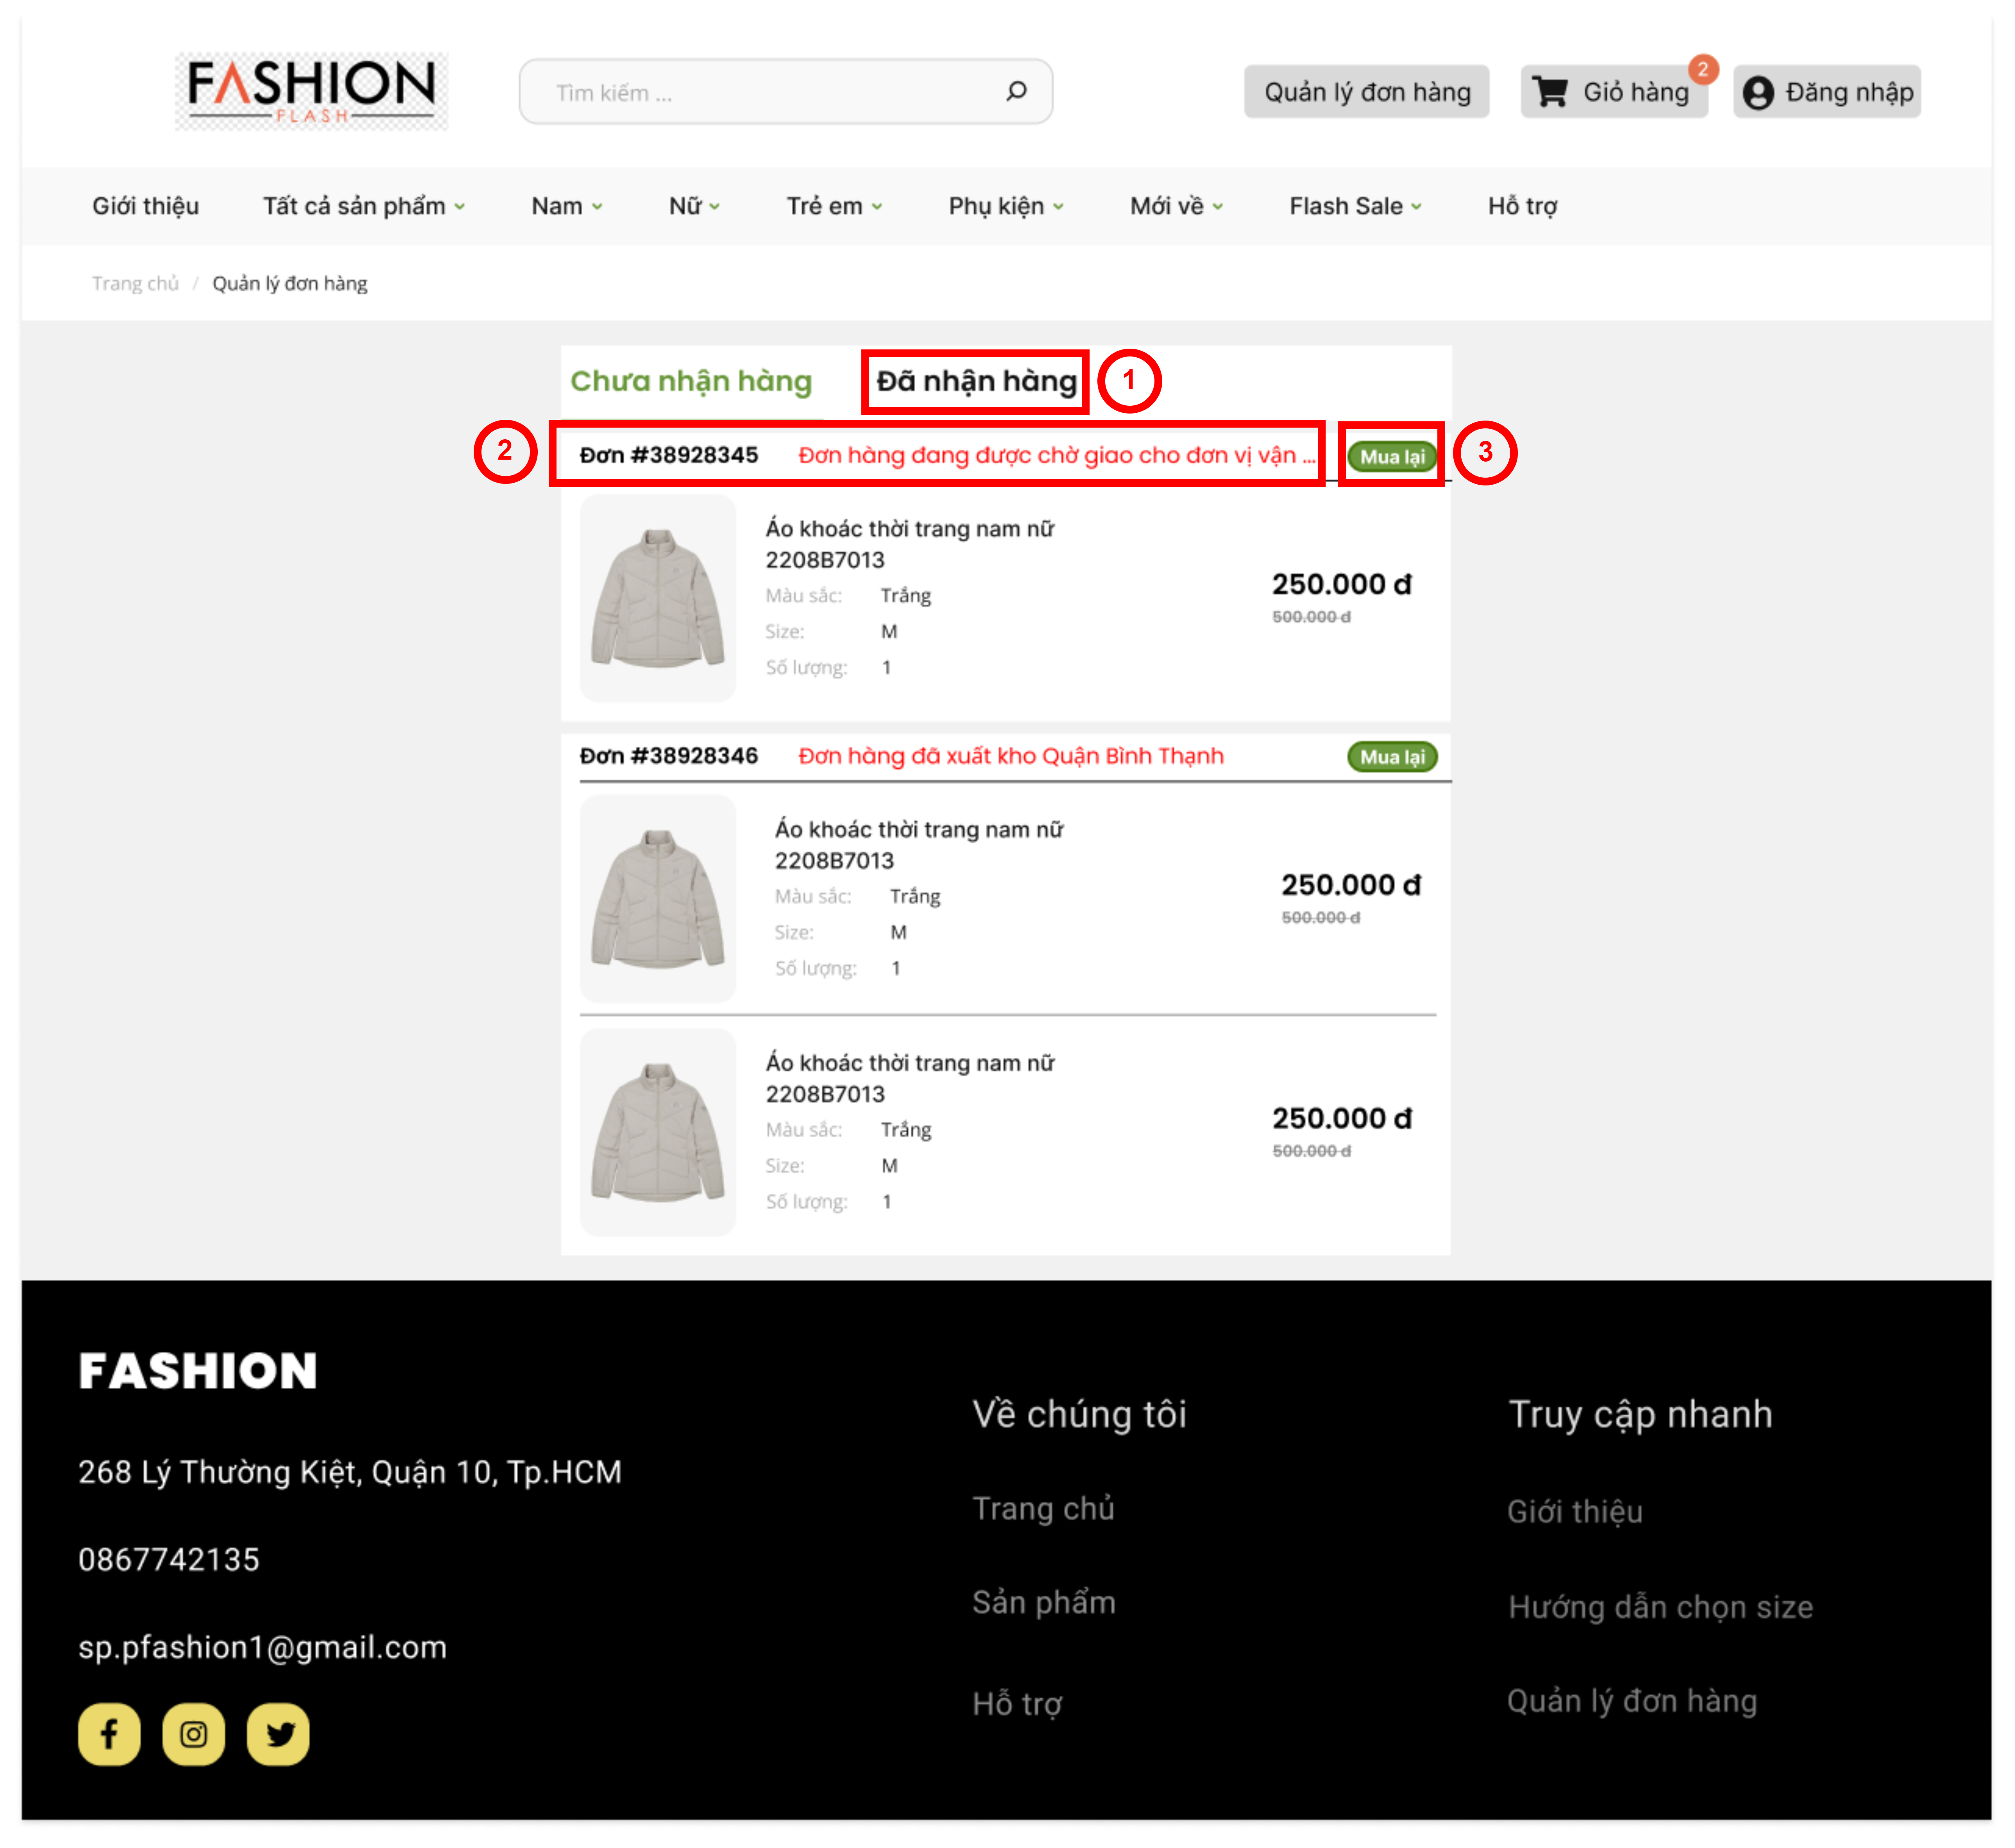
\includegraphics[width=5in]{img/UI/customer/customer_order.png}
        \label{13}
        \newline
        \caption{Giao diện quản lý đơn hàng của khách hàng.}
    \end{figure}
    \textbf{Mô tả:}  
    \begin{quote}
        \begin{enumerate}
            \item Chọn để xem danh sách các đơn hàng đã nhận.
            \item Chọn để xem thông tin chi tiết của đơn hàng.
            \item Chọn để thực hiện thêm lại các sản phẩm của đơn hàng vào giỏ hàng.
        \end{enumerate}
    \end{quote}   
        
    \subsubsection{Giao diện chi tiết đơn hàng}
    \begin{figure}[!htp]
        \centering
        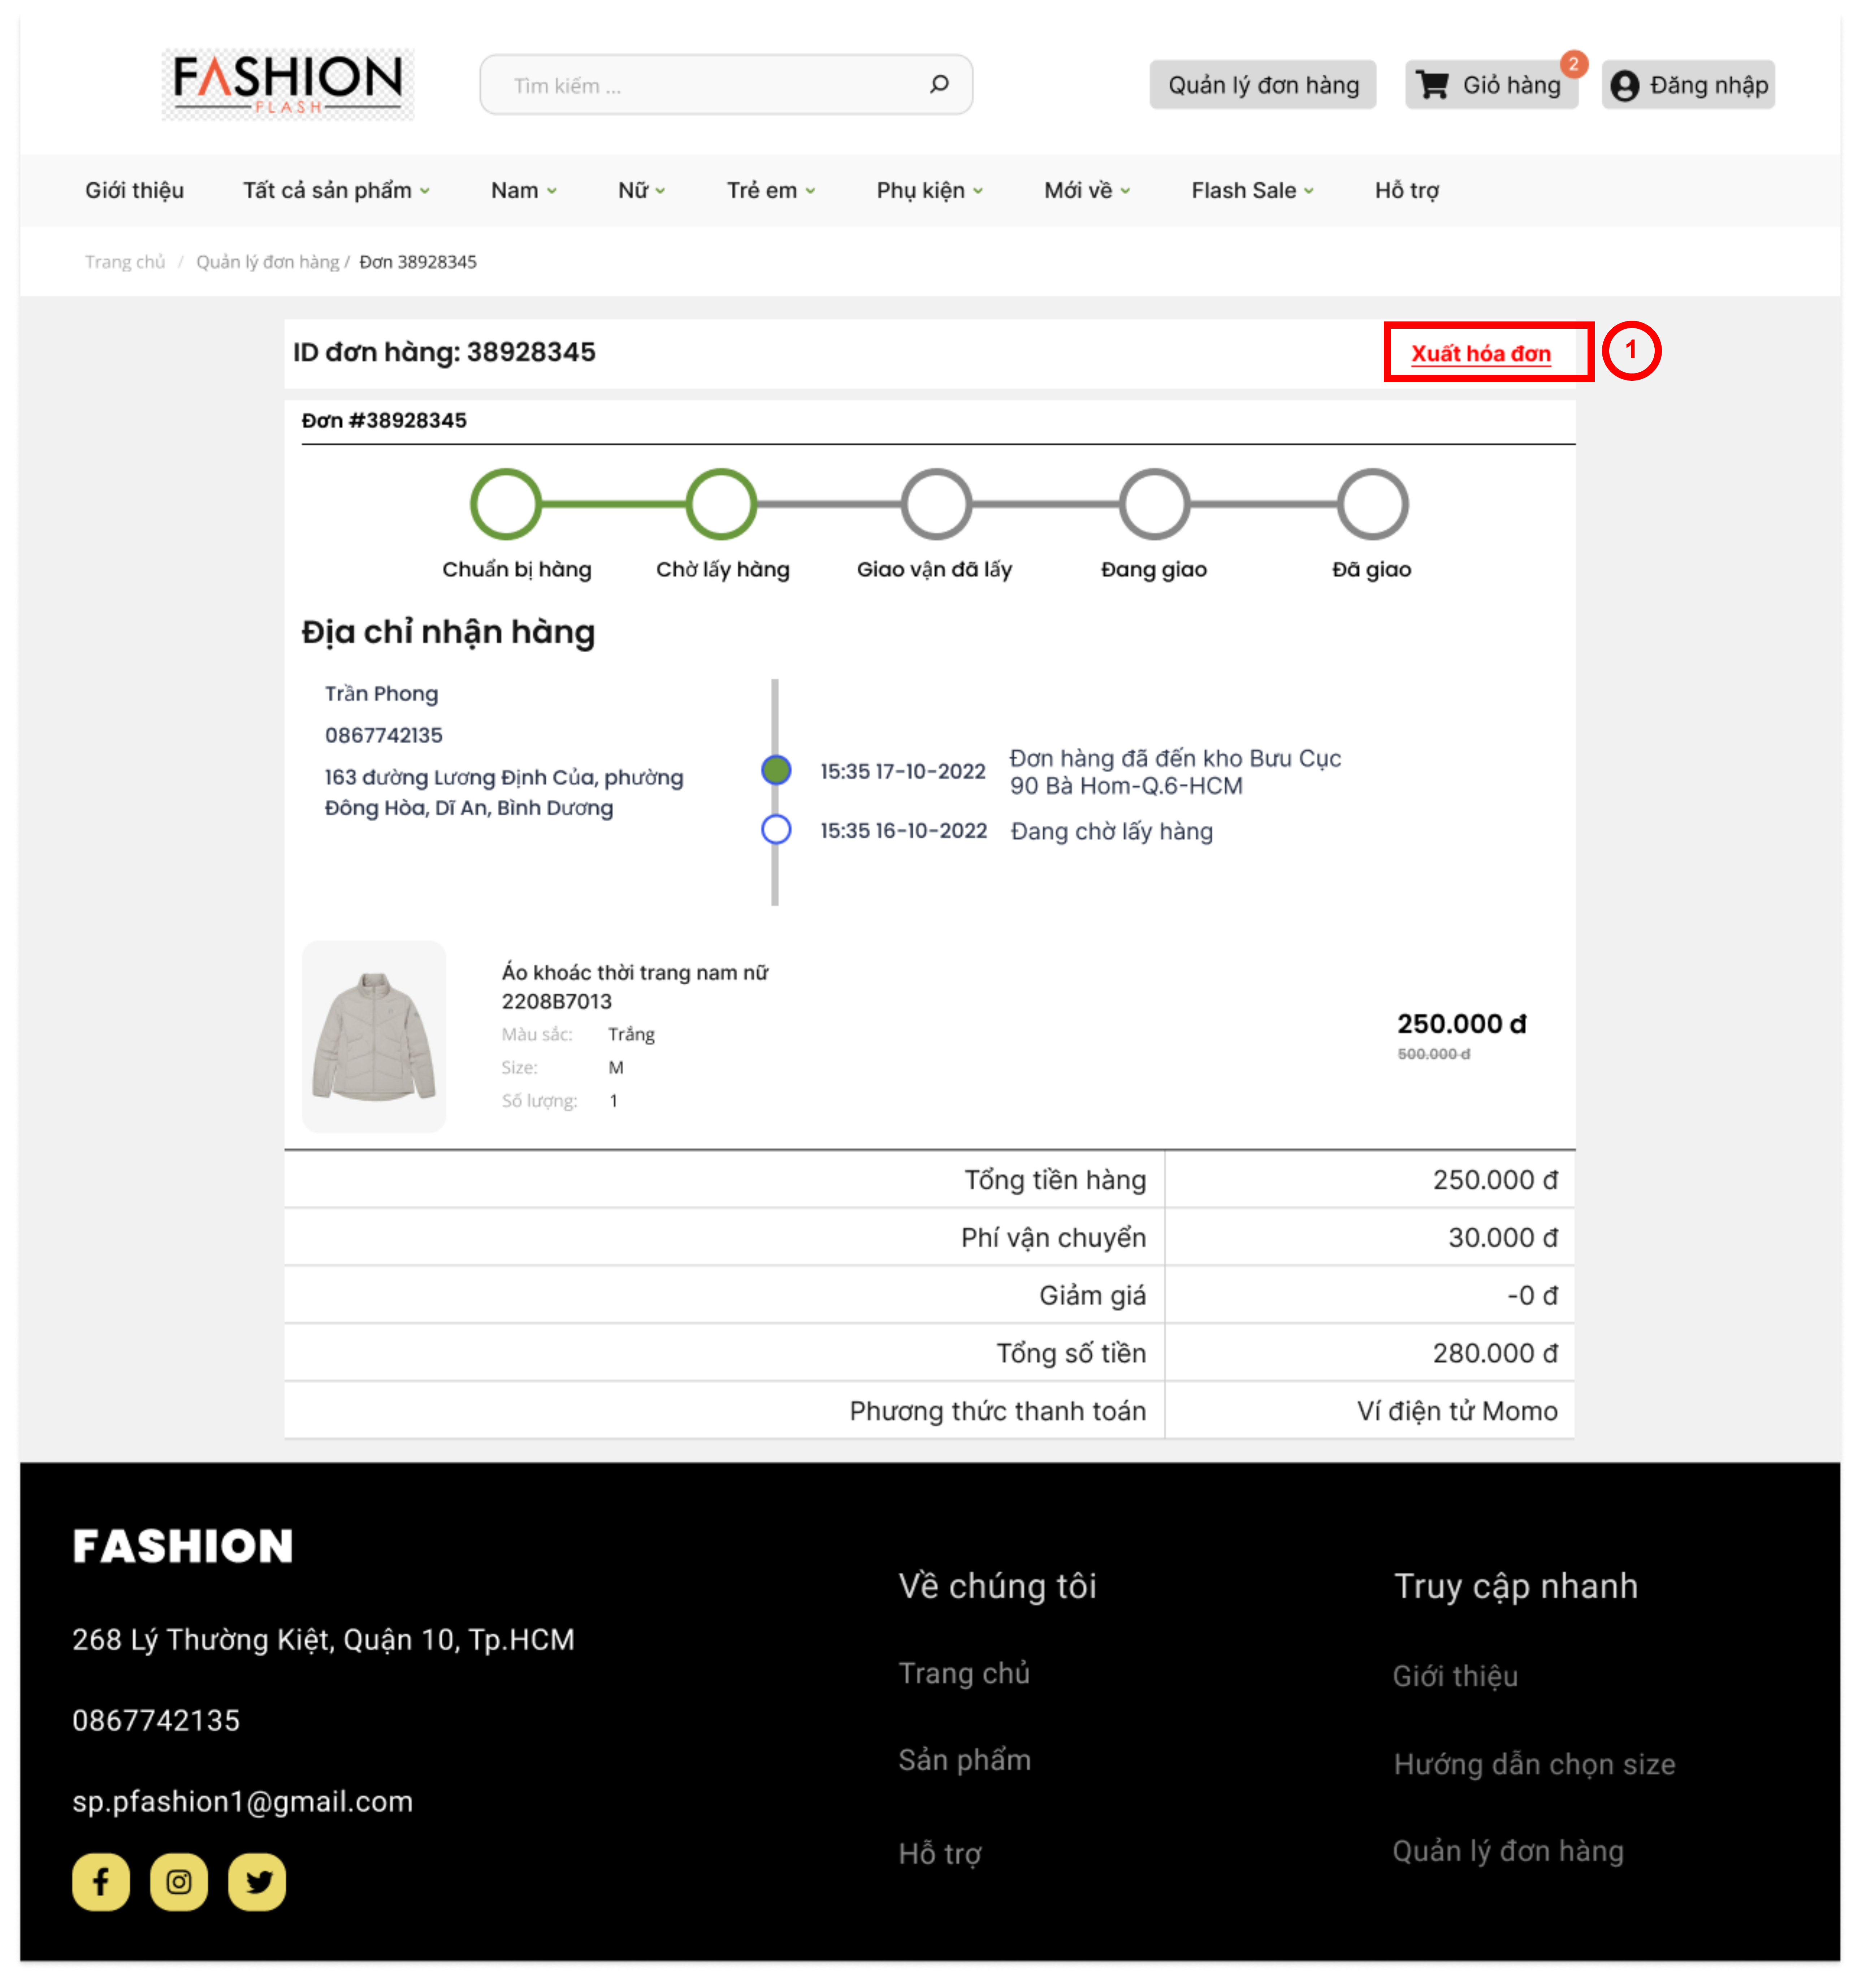
\includegraphics[width=5in]{img/UI/customer/order_detail.png}
        \label{14}
        \newline
        \caption{Giao diện xem chi tiết đơn hàng của khách hàng.}
    \end{figure}
    \textbf{Mô tả:}  
    \begin{quote}
        \begin{enumerate}
            \item Chọn để xuất hóa đơn cho đơn hàng.
        \end{enumerate}
    \end{quote}   
    
        
    \subsubsection{Giao diện thông tin khách hàng}
    \begin{figure}[!htp]
        \centering
        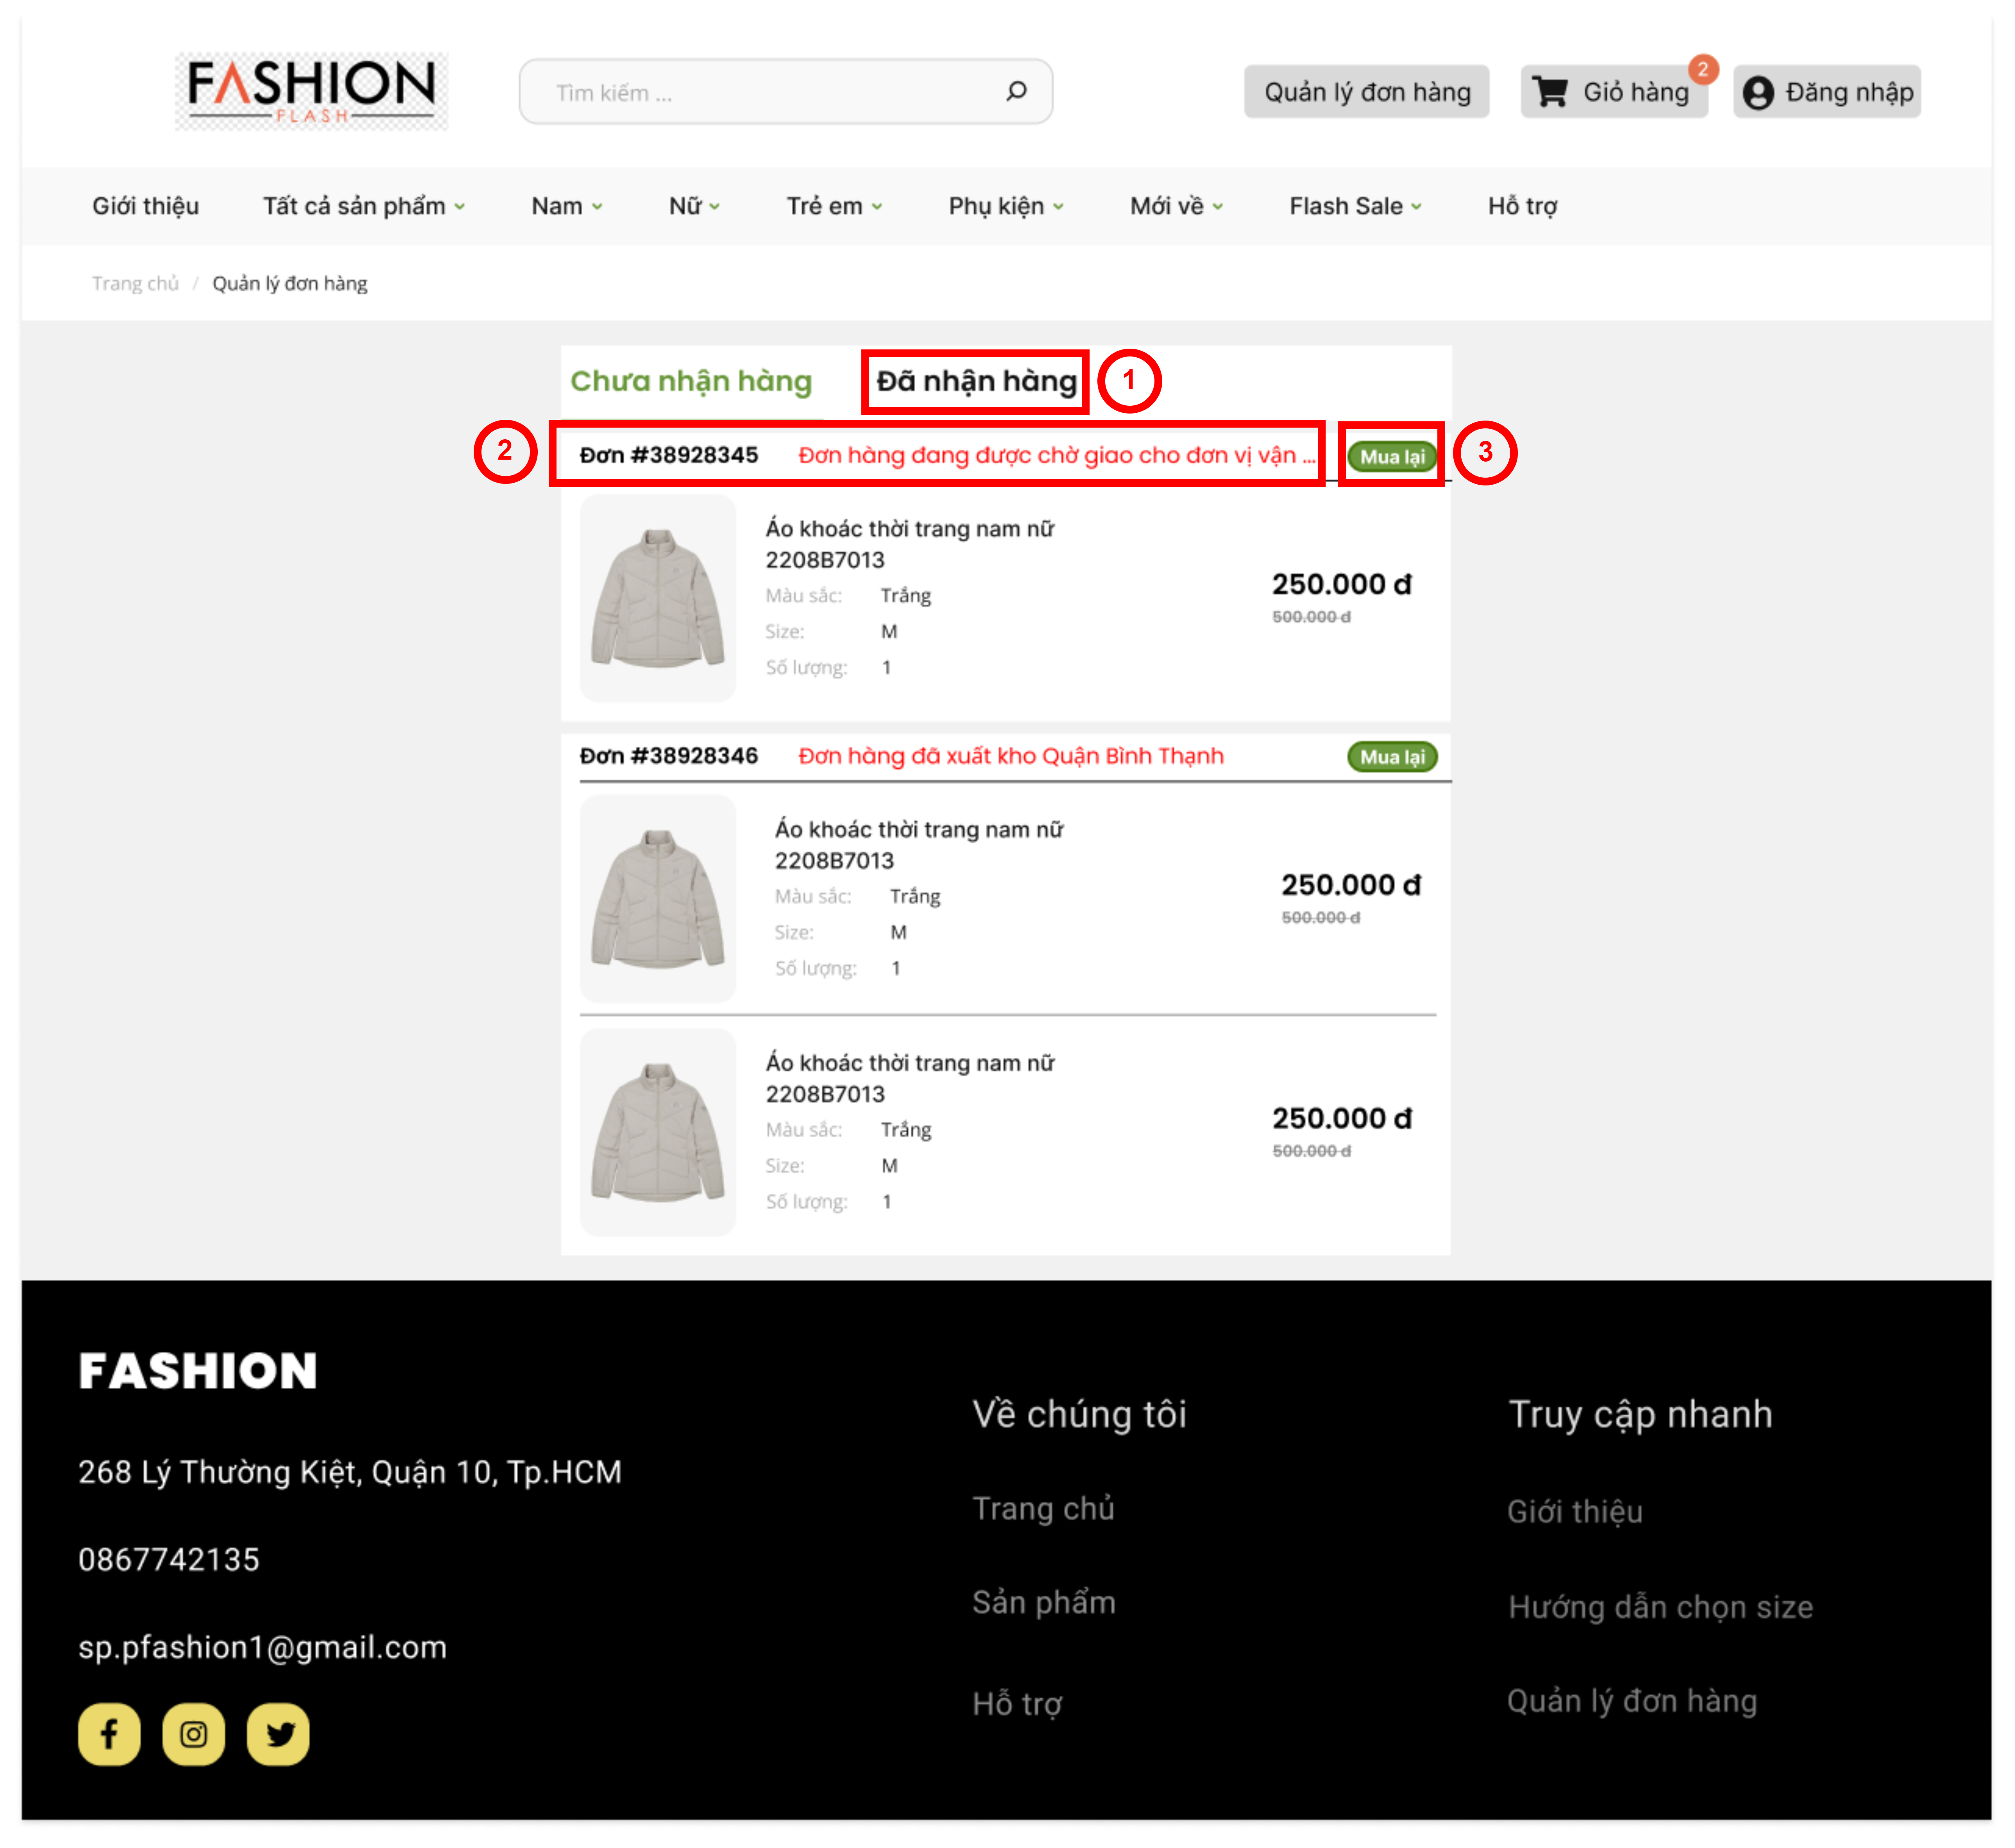
\includegraphics[width=5in]{img/UI/customer/customer_order.png}
        \label{15}
        \newline
        \caption{Giao diện xem thông tin tài khoản của khách hàng.}
    \end{figure}
    \textbf{Mô tả:}  
    \begin{quote}
        \begin{enumerate}
            \item Nhập để thay đổi tên của khách hàng.
            \item Nhập để thay đổi email của khách hàng.
            \item Chọn để thực hiện thay đổi mật khẩu của khách hàng.
            \item Nhập để thay đổi số nhà, đường của địa chỉ mặc định mà khách hàng muốn nhận hàng.
            \item Chọn để thay đổi phường/xã của địa chỉ mặc định mà khách hàng muốn nhận hàng.
            \item Chọn để thay đổi quận/huyện của địa chỉ mặc định mà khách hàng muốn nhận hàng.
            \item Chọn để thay đổi tỉnh/thành phố của địa chỉ mặc định mà khách hàng muốn nhận hàng.
            \item Chọn để thay đổi ảnh đại hình cho tài khoản của khách hàng.
        \end{enumerate}
    \end{quote}  
    Giao diện sau khi chọn "Đổi mật khẩu":
    \begin{figure}[!htp]
        \centering
        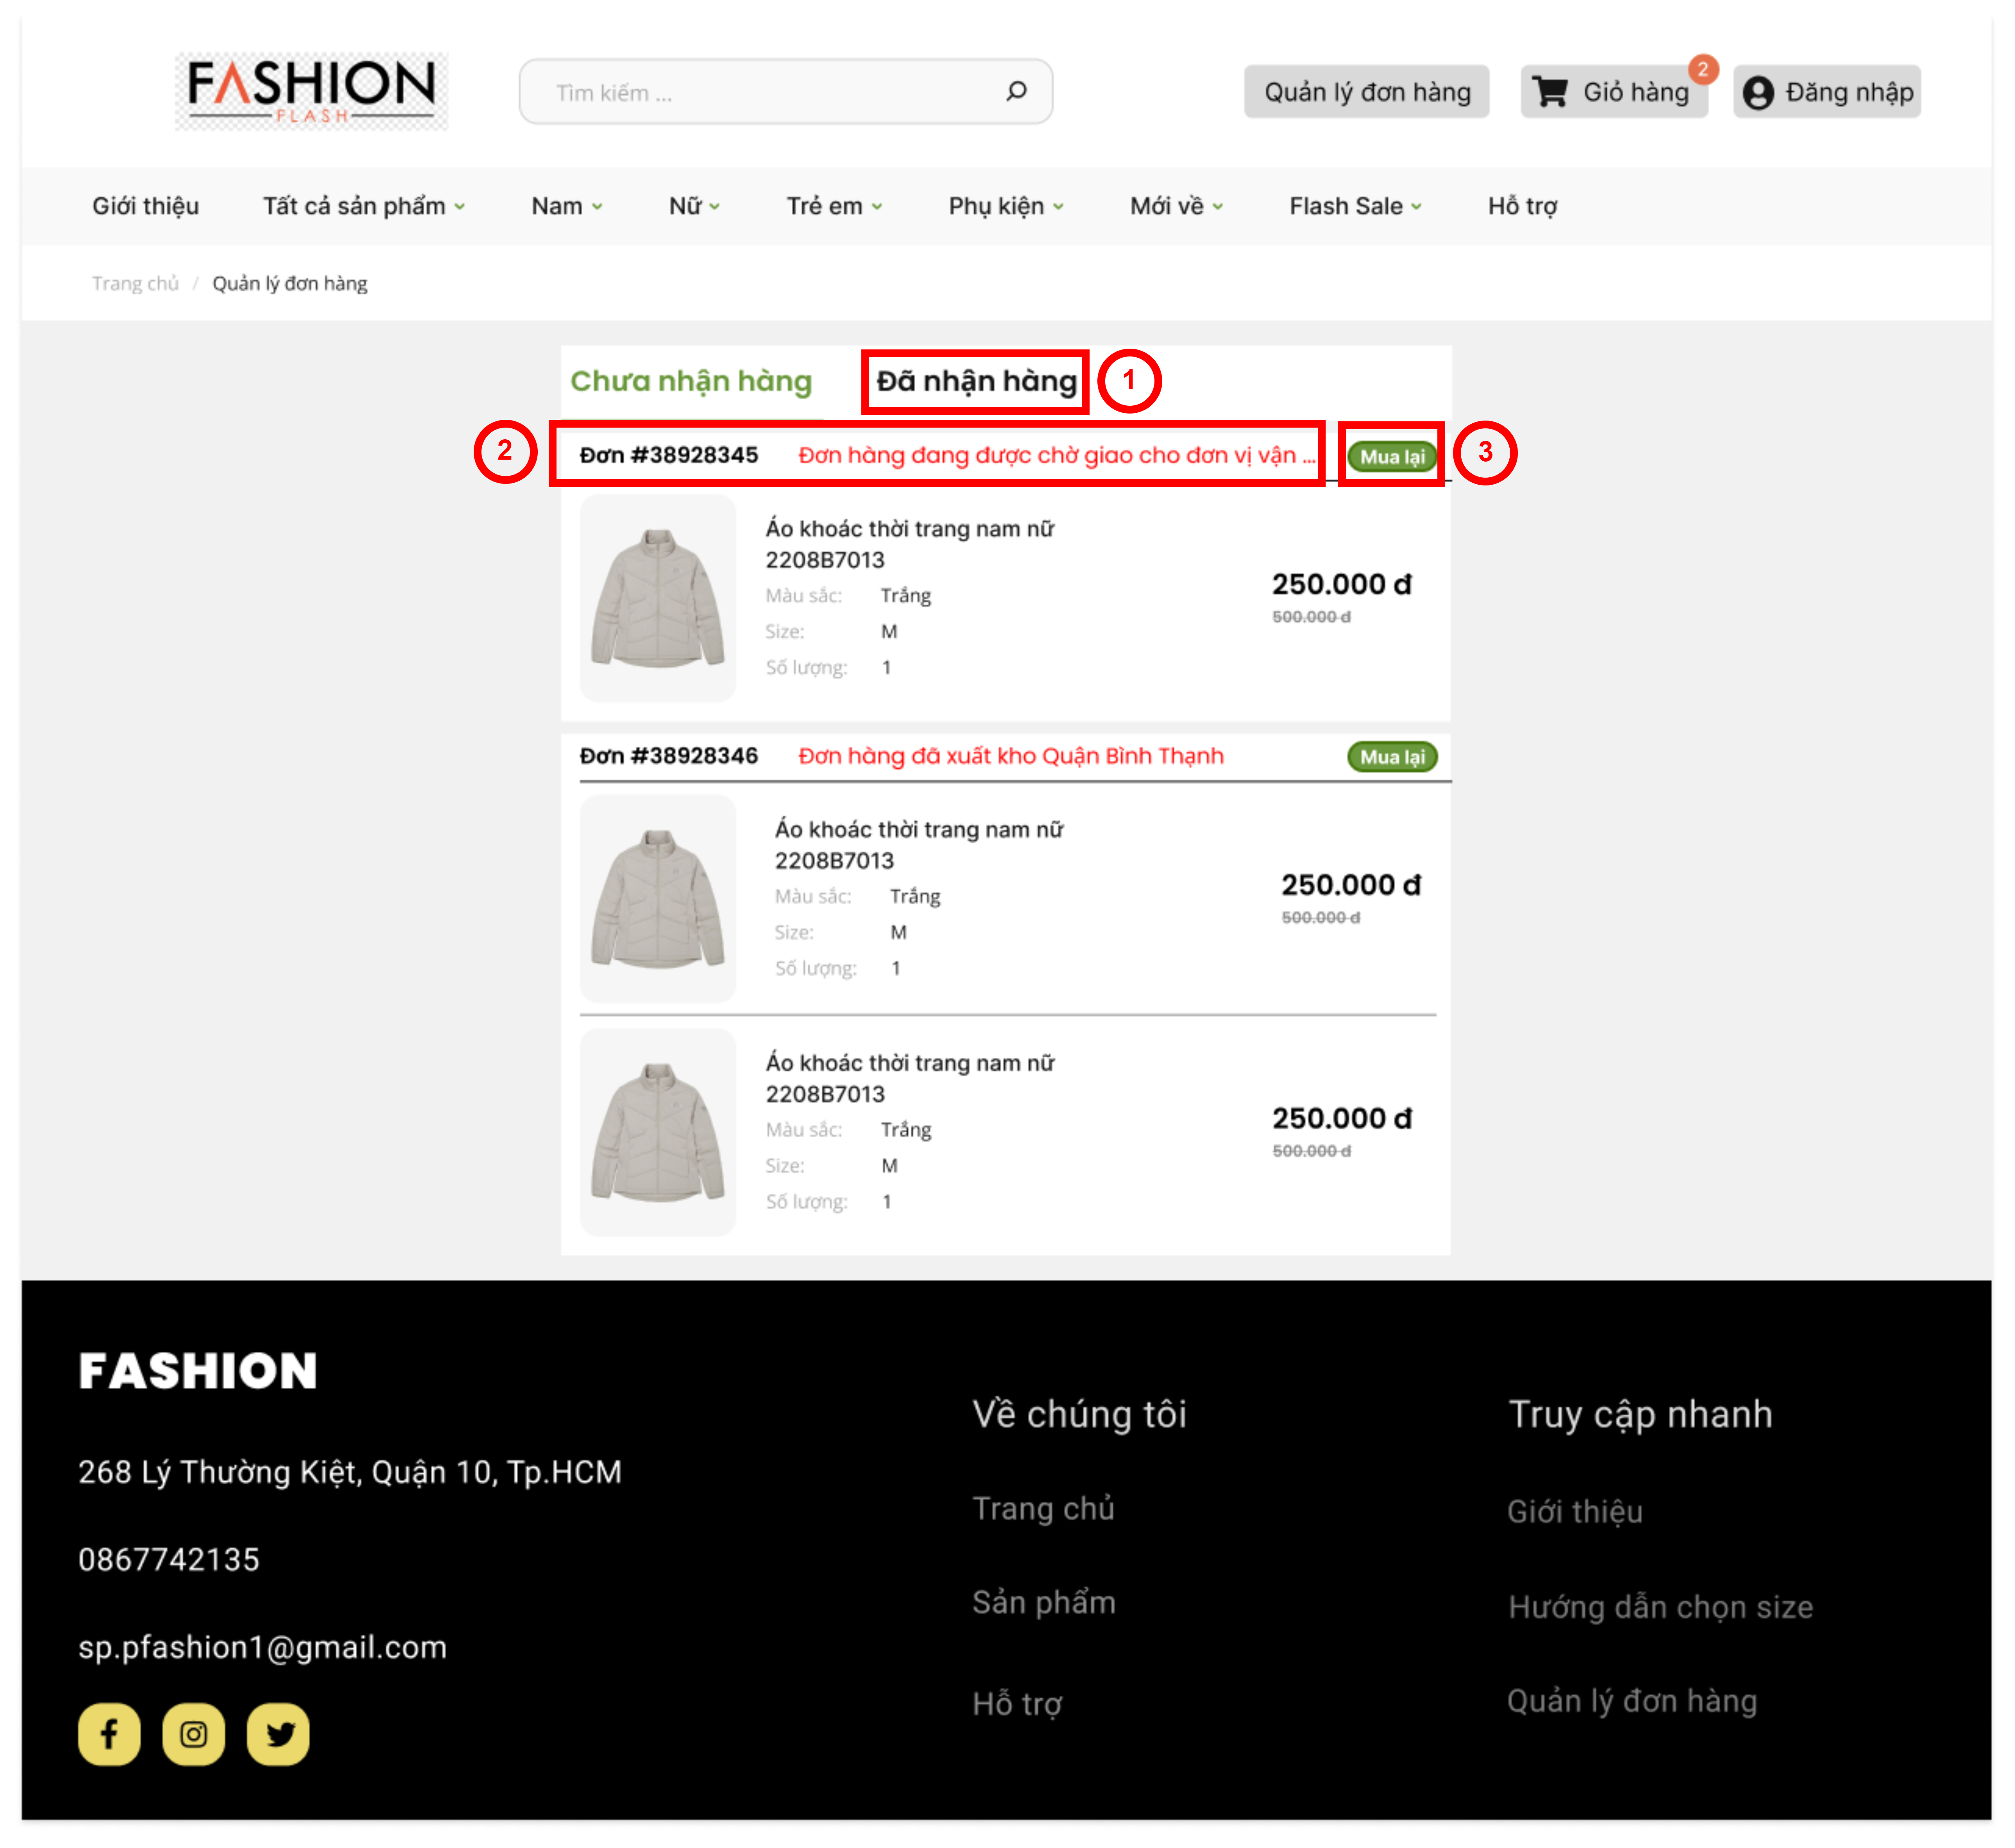
\includegraphics[width=5in]{img/UI/customer/customer_order.png}
        \label{16}
        \newline
        \caption{Giao diện đổi mật khẩu cho tài khoản.}
    \end{figure}
    \textbf{Mô tả:}  
    \begin{quote}
        \begin{enumerate}
            \item Nhập để điền mật khẩu cũ, yêu cầu tối thiểu 6 ký tự.
            \item Nhập để điền mật khẩu mới, yêu cầu tối thiểu 6 ký tự.
            \item Nhập để điền xác nhận mật khẩu mới, yêu cầu giống mật khẩu mới.
            \item Chọn để xác nhận thay đổi mật khẩu.
            \item Chọn để tắt màn hình khi không muốn thay đổi mật khẩu nữa.
        \end{enumerate}
    \end{quote}   
    
\subsection{Giao diện quản trị viên}
    \subsubsection{Chung}
        \begin{figure}[!htp]
            \centering
            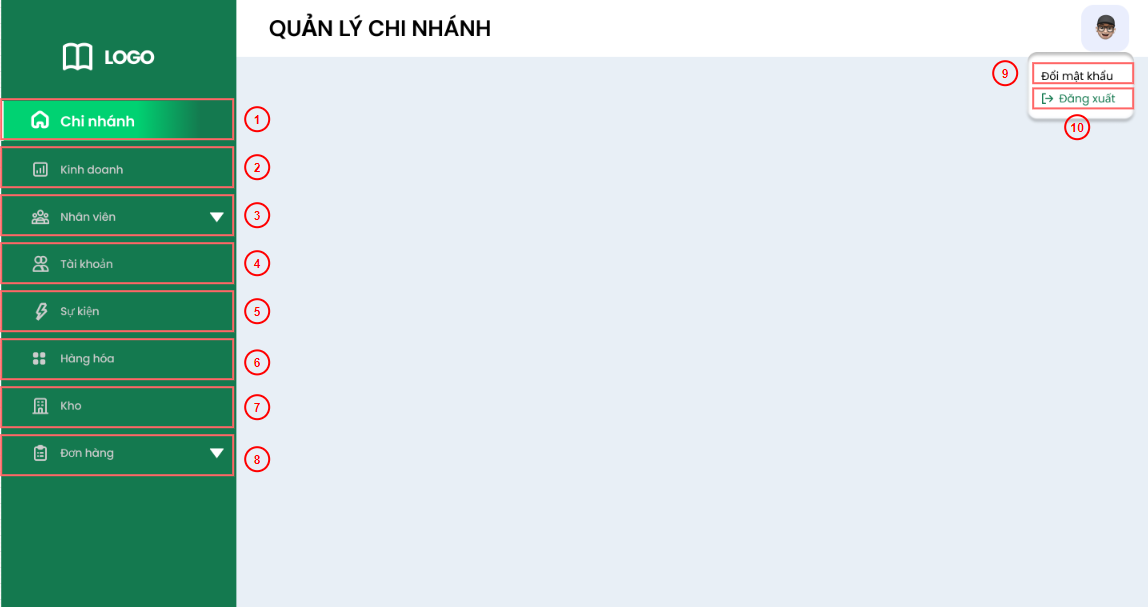
\includegraphics[width=10cm]{img/UI/admin/sidebar.png}
            \label{17}
            \newline
            \caption{Giao diện phần chung cho quản trị viên}
        \end{figure}
        \textbf{Mô tả:}  
        \begin{quote}
            \begin{enumerate}
                \item Chọn để đến "quản lý chi nhánh".
                \item Chọn để đến "quản lý hoạt động kinh doanh".
                \item Chọn để đến "quản lý nhân viên".
                \item Chọn để đến "quản lý tài khoản khách hàng".
                \item Chọn để đến "quản lý sự kiện".
                \item Chọn để đến "quản lý hàng hóa".
                \item Chọn để đến "quản lý kho".
                \item Chọn để đến "quản lý đơn hàng".
                \item Chọn để đổi mật khẩu.
                \item Chọn để đăng xuất.
            \end{enumerate}
        \end{quote}
        \subsubsubsection{Thay đổi mật khẩu}
            \begin{figure}[!htp]
                \centering
                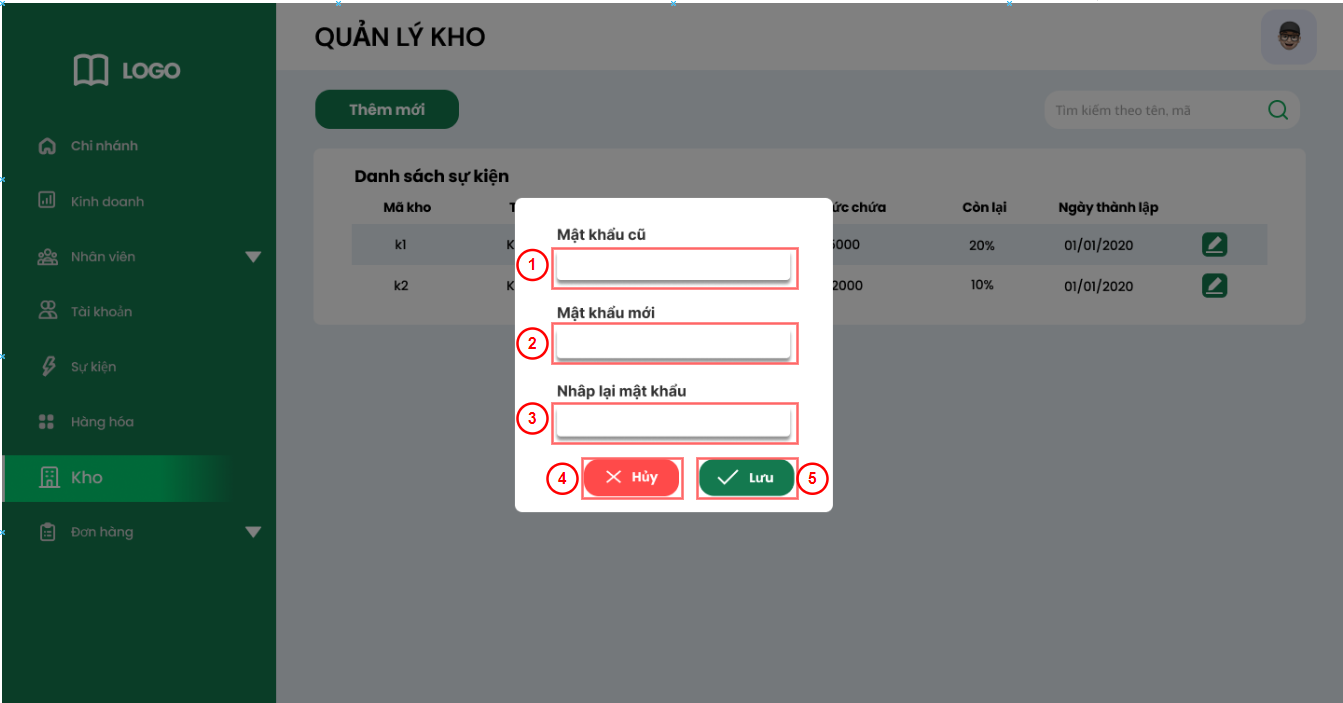
\includegraphics[width=10cm]{img/UI/admin/updatePassword.png}
                \label{18}
                \newline
                \caption{Giao diện cập nhật mật khẩu}
            \end{figure}
            \textbf{Mô tả:}  
            \begin{quote}
                \begin{enumerate}
                    \item Nhập mật khẩu cũ
                    \item Nhập mật khẩu mới
                    \item Nhập lại mật khẩu mới
                    \item Hủy cập nhật mật khẩu
                    \item Cập nhật mật khẩu
                \end{enumerate}
            \end{quote}
    
        \subsubsection{Quản lý chi nhánh}
            \begin{figure}[!htp]
                \centering
                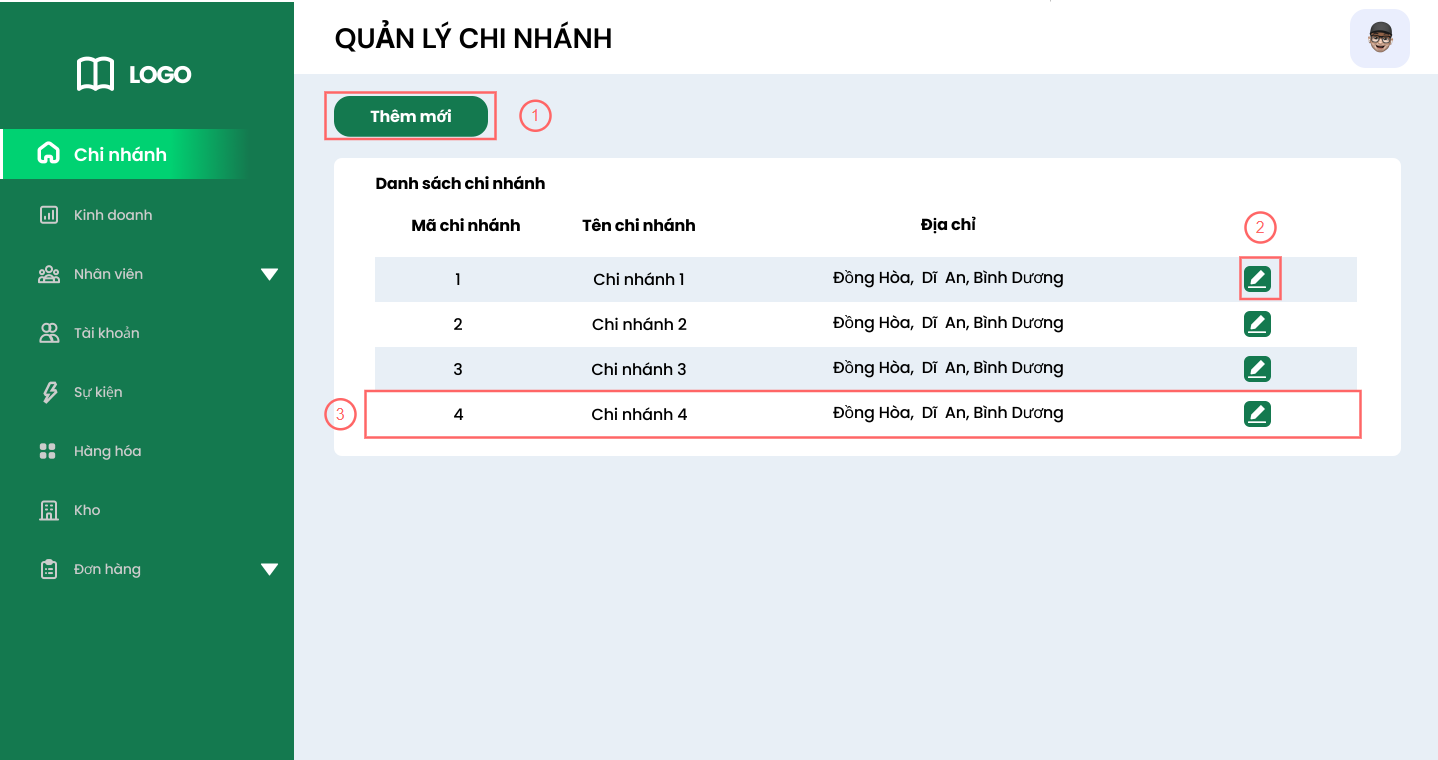
\includegraphics[width=10cm]{img/UI/admin/branch.png}
                \label{19}
                \newline
                \caption{Giao diện quản lý chi nhánh}
            \end{figure}
            \textbf{Mô tả:}  
            \begin{quote}
                \begin{enumerate}
                    \item Chọn để hiện form "thêm chi nhánh" mới
                    \item Chọn để hiện form "chỉnh sửa chi nhánh"
                    \item Chọn để xem thông tin "chi tiết chi nhánh"
                \end{enumerate}
            \end{quote}
                
            \subsubsubsection{Thêm, chỉnh sửa chi nhánh}
                \begin{figure}[!htp]
                    \centering
                    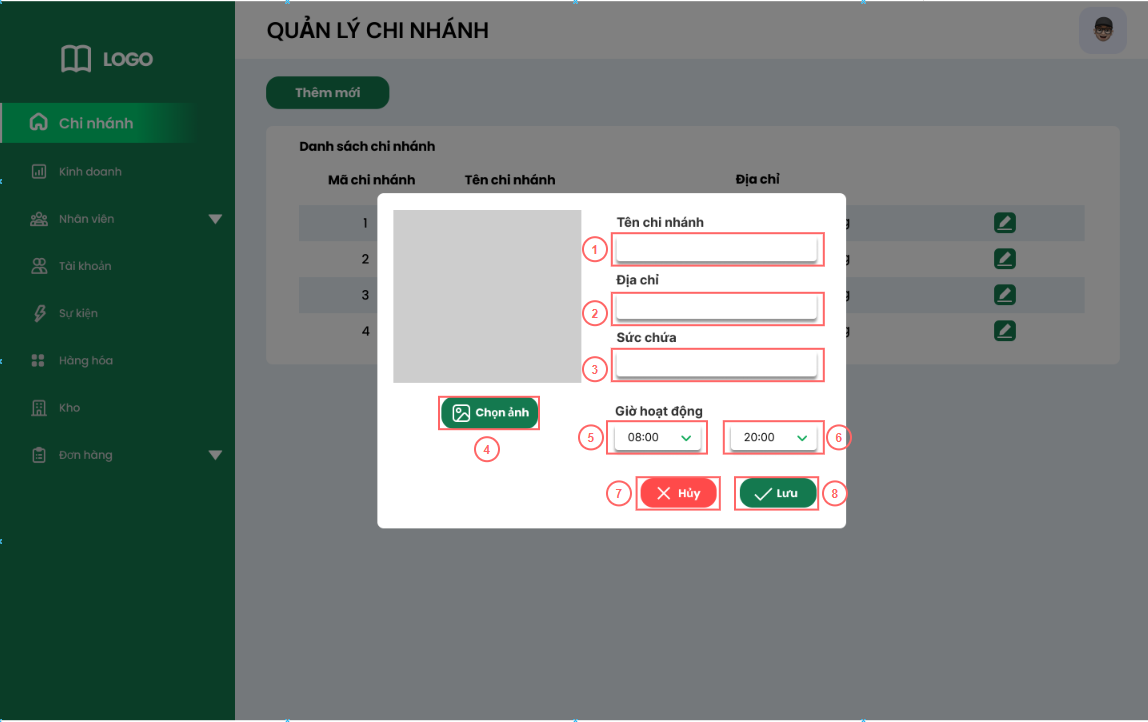
\includegraphics[width=10cm]{img/UI/admin/branch_add-edit.png}
                    \label{20}
                    \newline
                    \caption{Giao diện form thêm, chỉnh sửa chi nhánh}
                \end{figure}
                \textbf{Mô tả:}  
                \begin{quote}
                    \begin{enumerate}
                        \item Điền tên chi nhánh
                        \item Điền địa chỉ chi nhánh
                        \item Điền sức chứa chi nhánh
                        \item Chọn ảnh cho chi nhánh
                        \item Chọn giờ mở cửa của chi nhánh
                        \item Chọn giờ đóng cửa chi nhánh
                        \item Chọn để hủy hoạt động
                        \item Chọn để lưu thêm mới, chỉnh sửa chi nhánh
                    \end{enumerate}
                \end{quote}
        
            \subsubsubsection{Thông tin chi tiết chi nhánh}
                \begin{figure}[!htp]
                    \centering
                    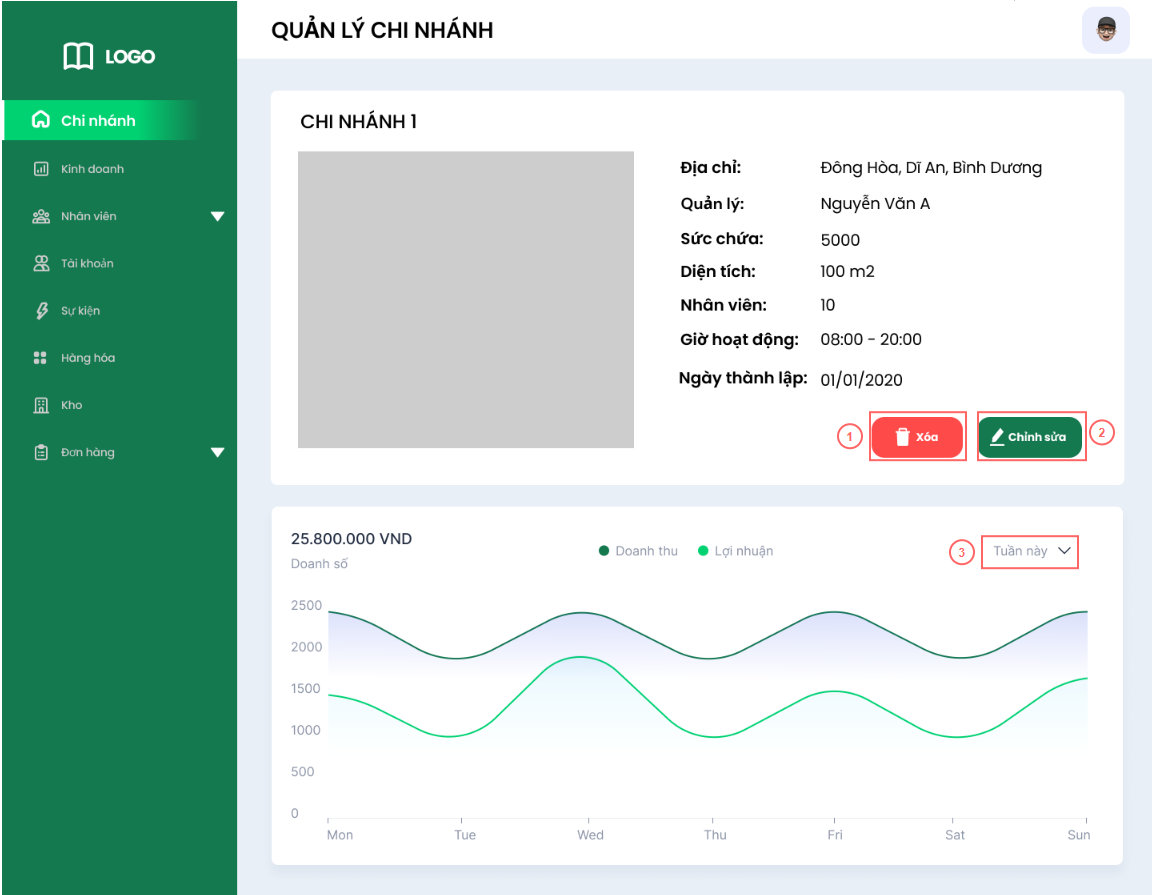
\includegraphics[width=10cm]{img/UI/admin/branch_detail.png}
                    \label{21}
                    \newline
                    \caption{Giao diện thông tin chi tiết chi nhánh}
                \end{figure}
                \textbf{Mô tả:}  
                \begin{quote}
                    \begin{enumerate}
                        \item Chọn để xóa chi nhánh
                        \item Chọn để hiện thị form "chỉnh sửa chi nhánh"
                        \item Chọn thời gia để hiện thị biểu đồ hoạt động tổng quát
                    \end{enumerate}
                \end{quote}
    
    \subsubsection{Quản lý hoạt động kinh doanh}
        \begin{figure}[!htp]
            \centering
            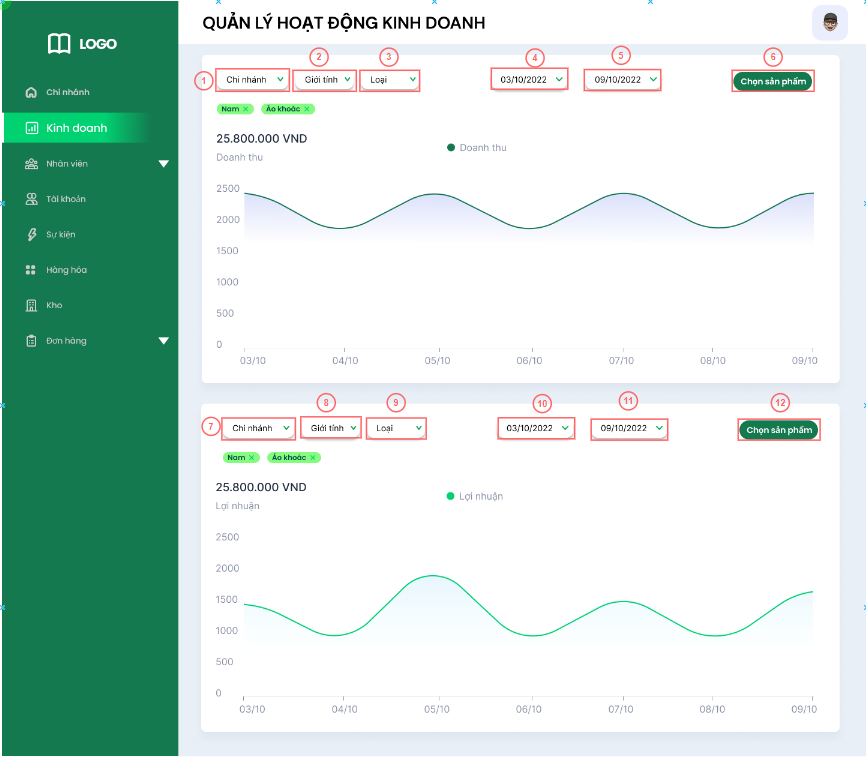
\includegraphics[width=10cm]{img/UI/admin/business.png}
            \label{22}
            \newline
            \caption{Giao diện quản lý hoạt động kinh doanh}
        \end{figure}
        \textbf{Mô tả:}  
        \begin{quote}
            \begin{enumerate}
                \item Chọn để lọc doanh thu theo chi nhánh 
                \item Chọn để lọc doanh thu theo giới tính
                \item Chọn để lọc doanh thu theo loại hàng
                \item Chọn để xác định  thời gian bắt đầu tính doanh thu
                \item Chọn để xác định thời gian kết thúc tính doanh thu
                \item Chọn để chọn sản phẩm để xem thống kê doanh thu
                \item Chọn để lọc lợi nhuận theo chi nhánh 
                \item Chọn để lọc lợi nhuận theo giới tính
                \item Chọn để lọc lợi nhuận theo loại hàng
                \item Chọn để xác định  thời gian bắt đầu tính lợi nhuận
                \item Chọn để xác định thời gian kết thúc tính lợi nhuận
                \item Chọn để chọn sản phẩm để xem thống kê lợi nhuận
            \end{enumerate}
        \end{quote}
    
    \subsubsection{Quản lý nhân viên}
        \begin{figure}[!htp]
            \centering
            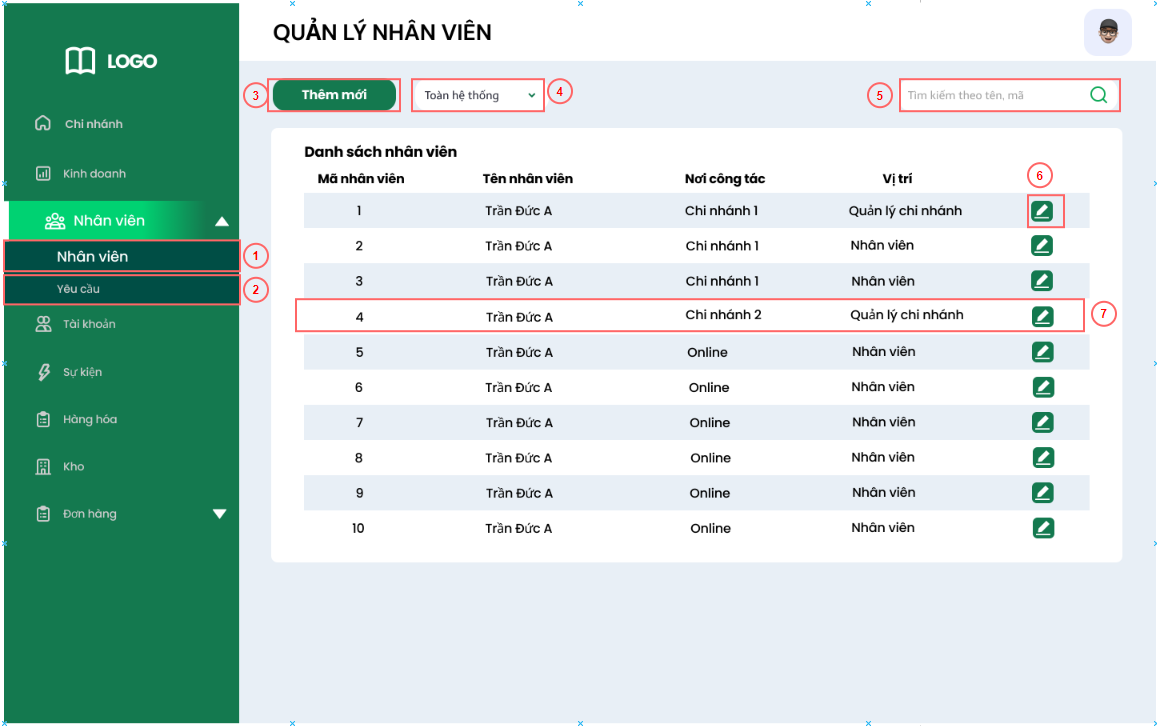
\includegraphics[width=10cm]{img/UI/admin/staff.png}
            \label{23}
            \newline
            \caption{Giao diện quản lý nhân viên}
        \end{figure}
        \textbf{Mô tả:}  
        \begin{quote}
            \begin{enumerate}
                \item Chọn để xem quản lý nhân viên
                \item Chọn để xem yêu cầu từ cấp dưới gửi lên
                \item Chọn để thêm nhân viên mới
                \item Chọn để lọc nhân viên theo chi nhánh
                \item Nhập để tìm kiếm nhân viên theo mã, tên
                \item Chọn để xem thông tin chi tiết nhân viên
            \end{enumerate}
        \end{quote}
        \subsubsubsection{Thêm, chỉnh sửa nhân viên}
            \begin{figure}[!htp]
                \centering
                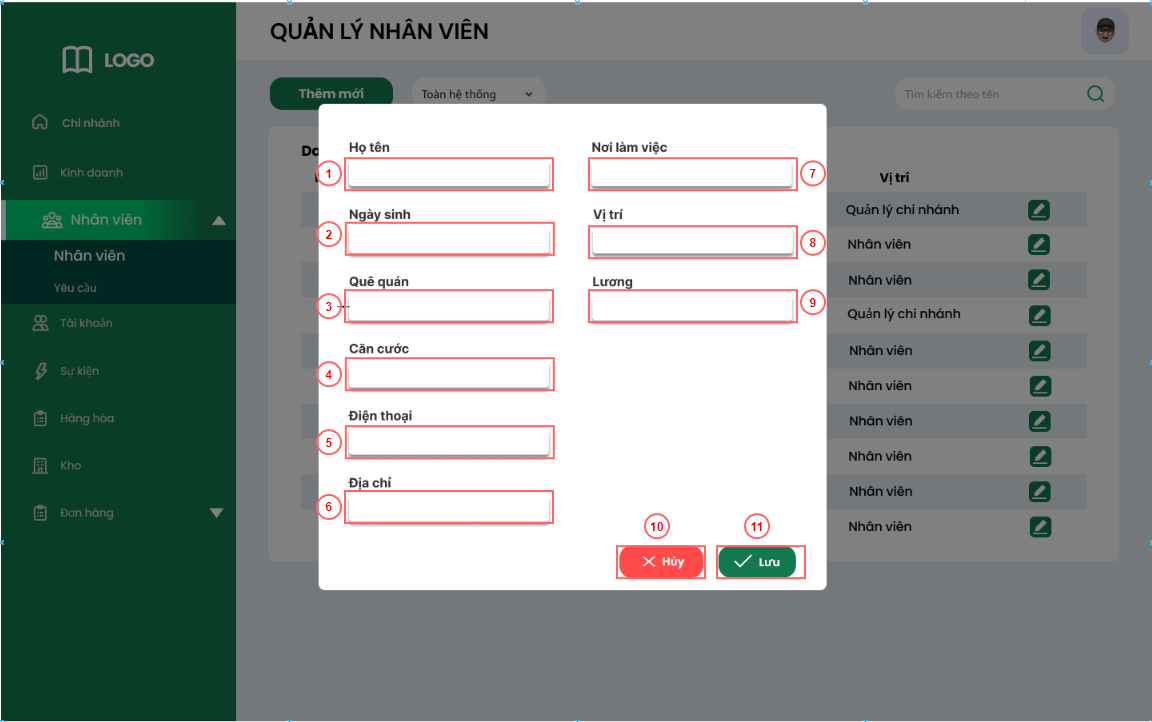
\includegraphics[width=10cm]{img/UI/admin/staff_edit_add.png}
                \label{24}
                \newline
                \caption{Giao diện thêm, chỉnh sửa nhân viên}
            \end{figure}
            \textbf{Mô tả:}  
            \begin{quote}
                \begin{enumerate}
                    \item Nhập họ tên nhân viên
                    \item Chọn ngày sinh nhân viên
                    \item Nhập quê quán nhân viên
                    \item Nhập căn cước nhân viên
                    \item Nhập số điện thoại nhân viên
                    \item Nhập địa chỉ nhân viên
                    \item Chọn nơi làm việc nhân viên
                    \item Chọm vị trí nhân viên
                    \item Nhập lương nhân viên
                    \item Chọn hủy hoạt động
                    \item Chọn lưu nhân viên mới, thông tin chỉnh sửa 
                \end{enumerate}
            \end{quote}
        \subsubsubsection{Thông tin chi tiết nhân viên}
            \begin{figure}[!htp]
                \centering
                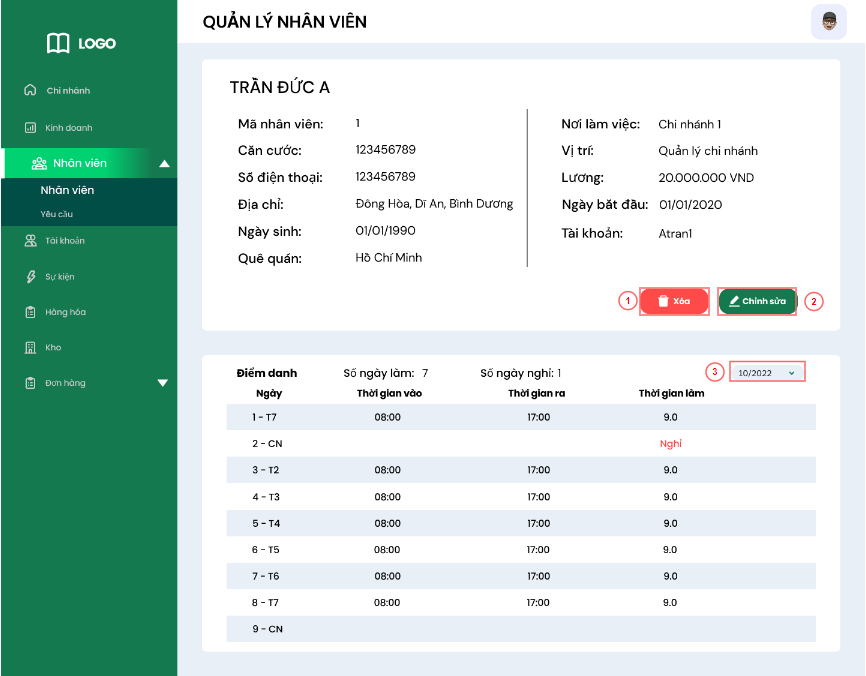
\includegraphics[width=10cm]{img/UI/admin/staff_detail.png}
                \label{25}
                \newline
                \caption{Giao diện thông tin chi tiết nhân viên}
            \end{figure}
            \textbf{Mô tả:}  
            \begin{quote}
                \begin{enumerate}
                    \item Chọn để xóa nhân viên
                    \item Chọn để hiện thị form chỉnh sửa nhân viên
                    \item Chọn tháng để xem lịch làm việc của nhân viên
                    
                \end{enumerate}
            \end{quote}
        
        \subsubsubsection{Quản lý yêu cầu nhân viên}
            \begin{figure}[!htp]
                \centering
                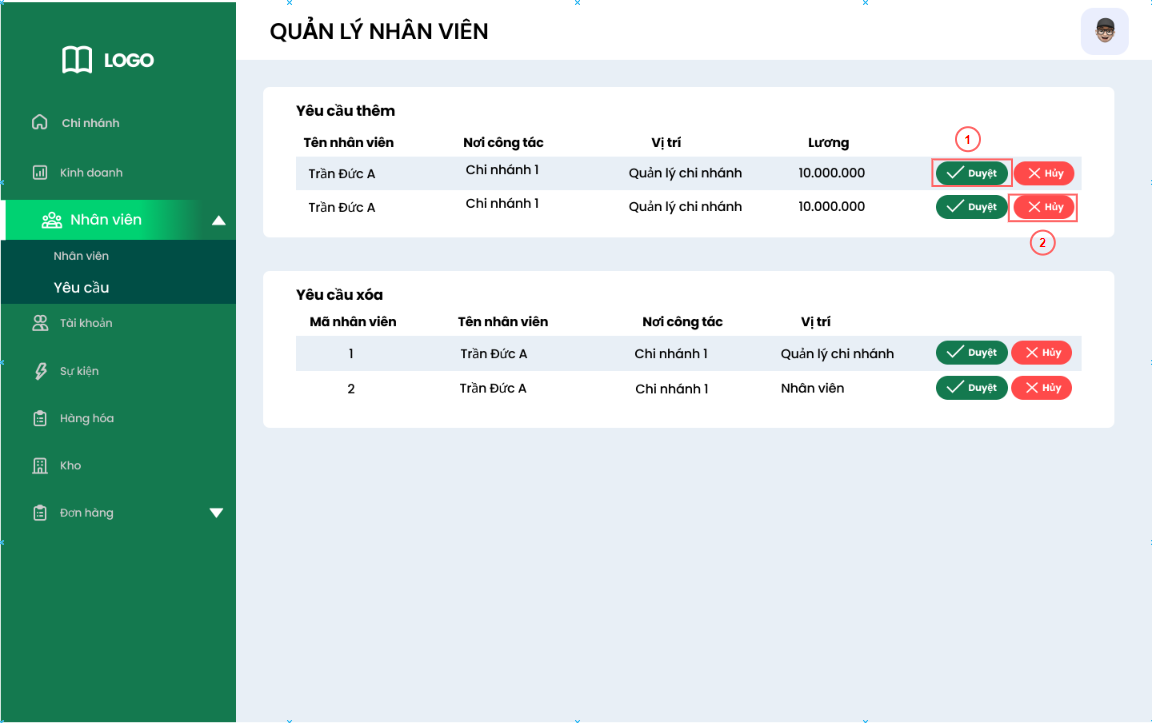
\includegraphics[width=10cm]{img/UI/admin/staff_request.png}
                \label{26}
                \newline
                \caption{Giao diện quản lý yêu cầu nhân viên}
            \end{figure}
            \textbf{Mô tả:}  
            \begin{quote}
                \begin{enumerate}
                    \item Chọn để duyệt yêu cầu
                    \item Chọn để xóa yêu cầu
                \end{enumerate}
            \end{quote}
        
        \subsubsubsection{Yêu cầu thêm nhân viên}
            \begin{figure}[!htp]
                \centering
                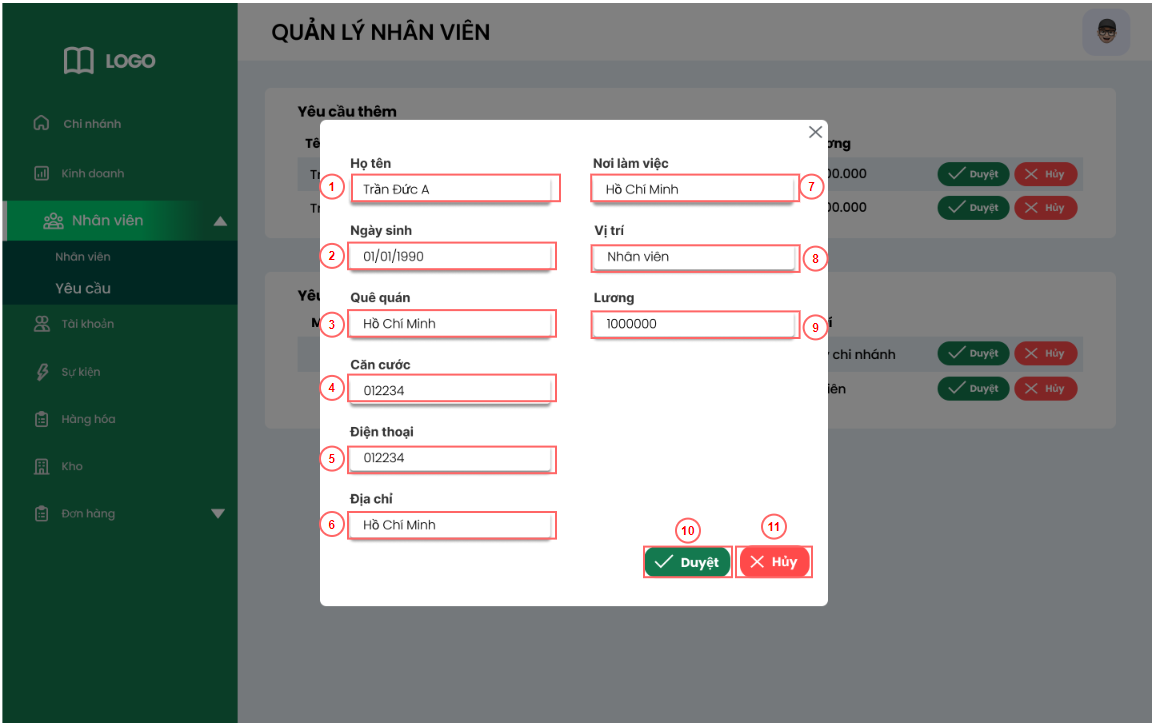
\includegraphics[width=10cm]{img/UI/admin/staff_request_add.png}
                \label{27}
                \newline
                \caption{Giao diện yêu cầu thêm nhân viên}
            \end{figure}
            \textbf{Mô tả:}  
            \begin{quote}
                \begin{enumerate}
                    \item Nhập họ tên nhân viên
                    \item Chọn ngày sinh nhân viên
                    \item Nhập quê quán nhân viên
                    \item Nhập căn cước nhân viên
                    \item Nhập số điện thoại nhân viên
                    \item Nhập địa chỉ nhân viên
                    \item Chọn nơi làm việc nhân viên
                    \item Chọm vị trí nhân viên
                    \item Nhập lương nhân viên
                    \item Chọn để duyệt yêu cầu
                    \item Chọn để xóa yêu cầu
                \end{enumerate}
            \end{quote}
        
        \subsubsubsection{Yêu cầu xóa nhân viên}
            \begin{figure}[!htp]
                \centering
                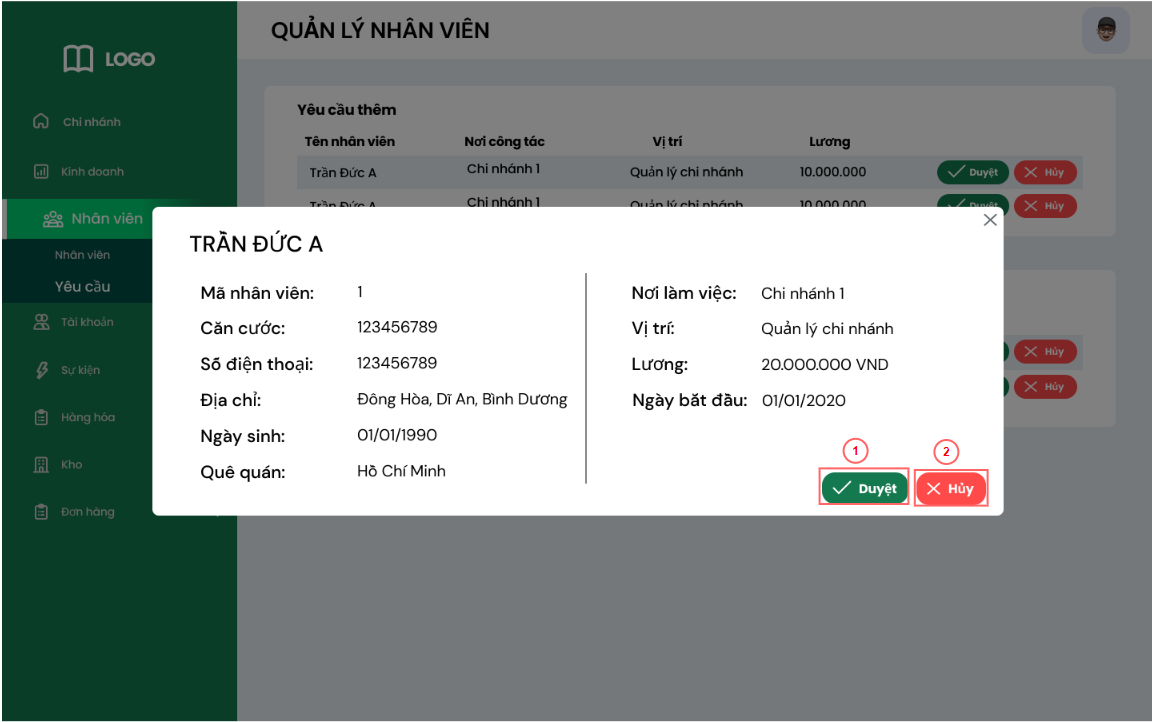
\includegraphics[width=10cm]{img/UI/admin/staff_request_delete.png}
                \label{28}
                \newline
                \caption{Giao diện yêu cầu xóa nhân viên}
            \end{figure}
            \textbf{Mô tả:}  
            \begin{quote}
                \begin{enumerate}
                    \item Chọn để duyệt yêu cầu
                    \item Chọn để xóa yêu cầu
                \end{enumerate}
            \end{quote}
        
    \subsubsection{Quản lý tài khoản}
        \begin{figure}[!htp]
            \centering
            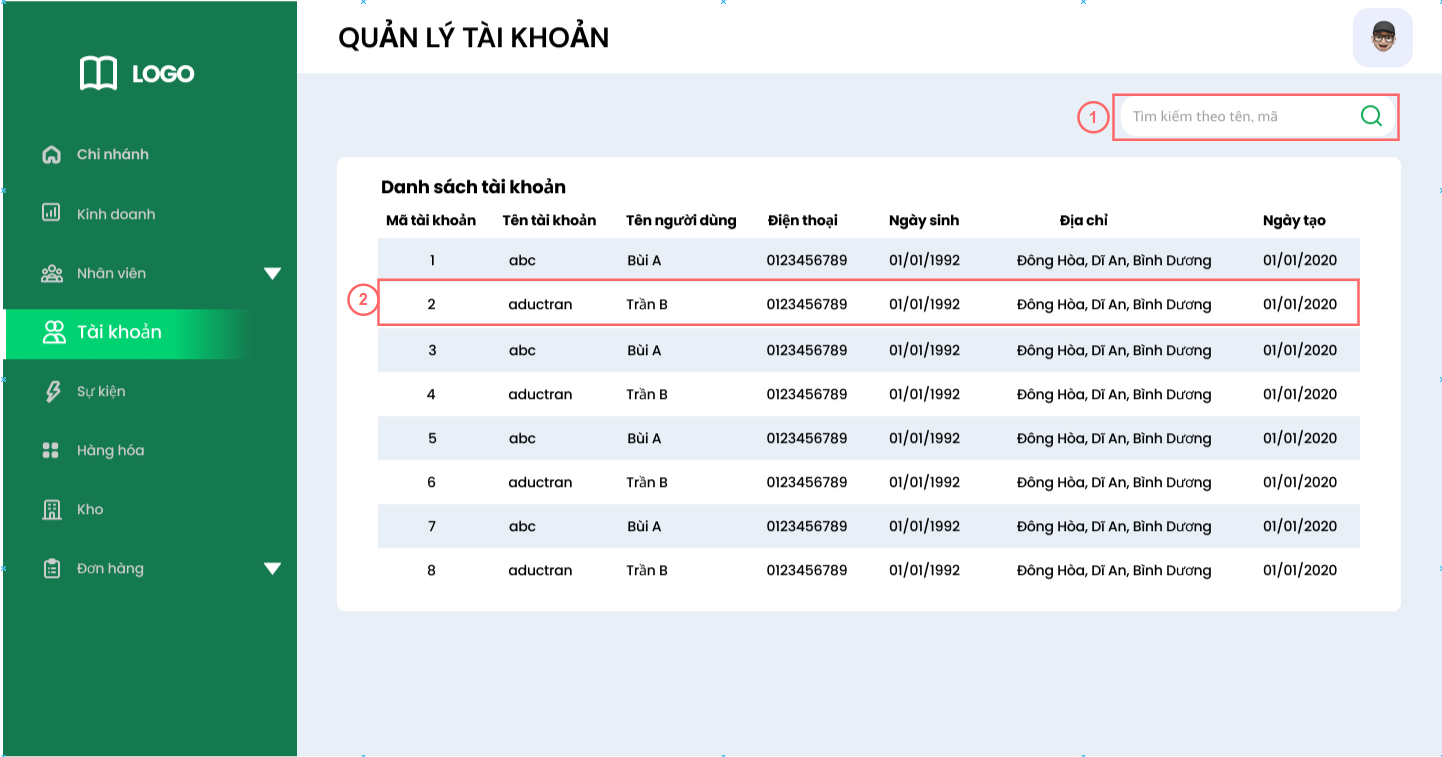
\includegraphics[width=10cm]{img/UI/admin/account.png}
            \label{29}
            \newline
            \caption{Giao diện quản lý tài khoản}
        \end{figure}
        \textbf{Mô tả:}  
        \begin{quote}
            \begin{enumerate}
                \item Nhập để tìm kiếm tài khoản theo Id, username
                \item Chọn để xem "thông tin chi tiết tài khoản"
            \end{enumerate}
        \end{quote}
        \subsubsubsection{Thông tin chi tiết tài khoản}
            \begin{figure}[!htp]
                \centering
                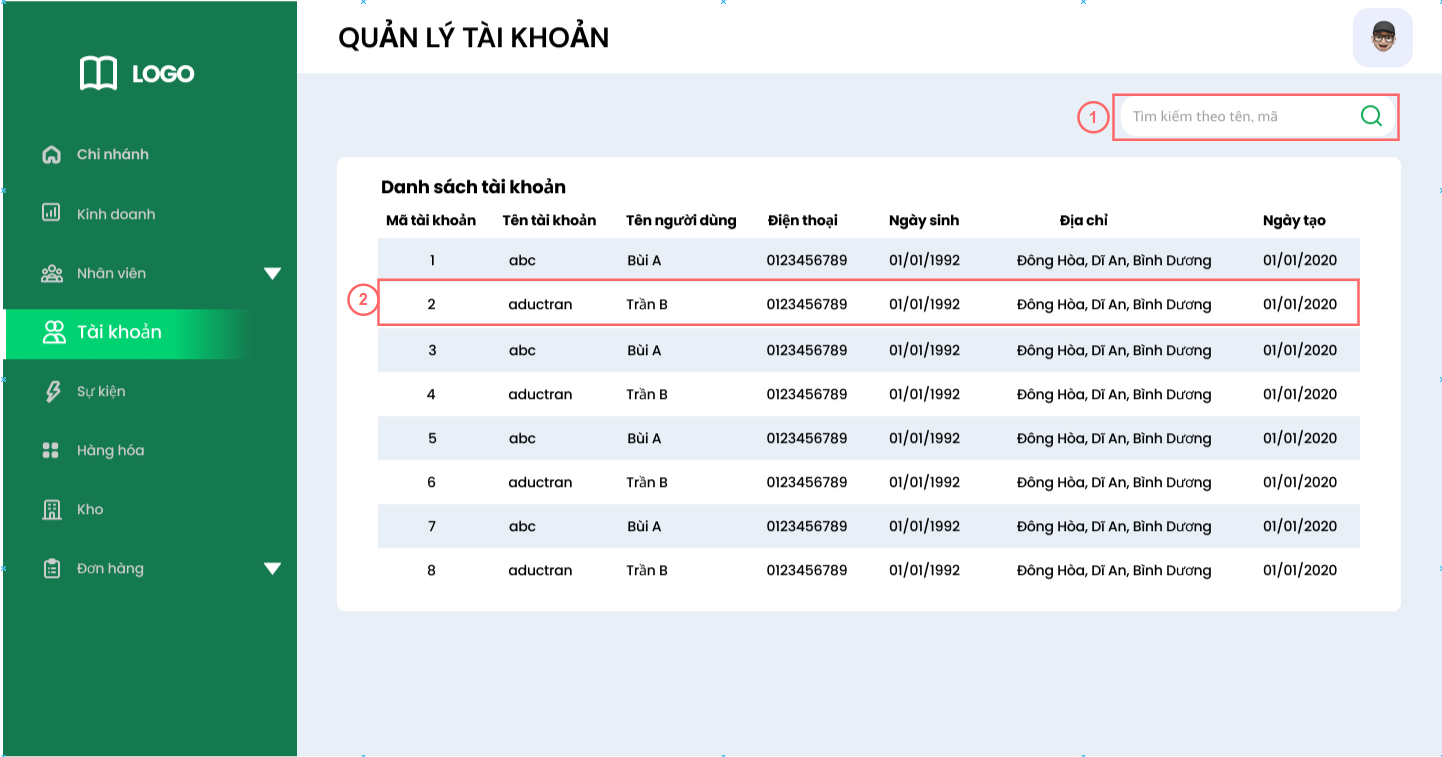
\includegraphics[width=10cm]{img/UI/admin/account.png}
                \label{30}
                \newline
                \caption{Giao diện thông tin chi tiết tài khoản}
            \end{figure}
            \textbf{Mô tả:}  
            \begin{quote}
                \begin{enumerate}
                    \item Chọn tháng xem danh sách đơn khách hàng
                    \item Chọn để xem thông tin chi tiết đơn
                \end{enumerate}
            \end{quote}
        \subsubsubsection{Thông tin chi tiết đơn hàng}
            \begin{figure}[!htp]
                \centering
                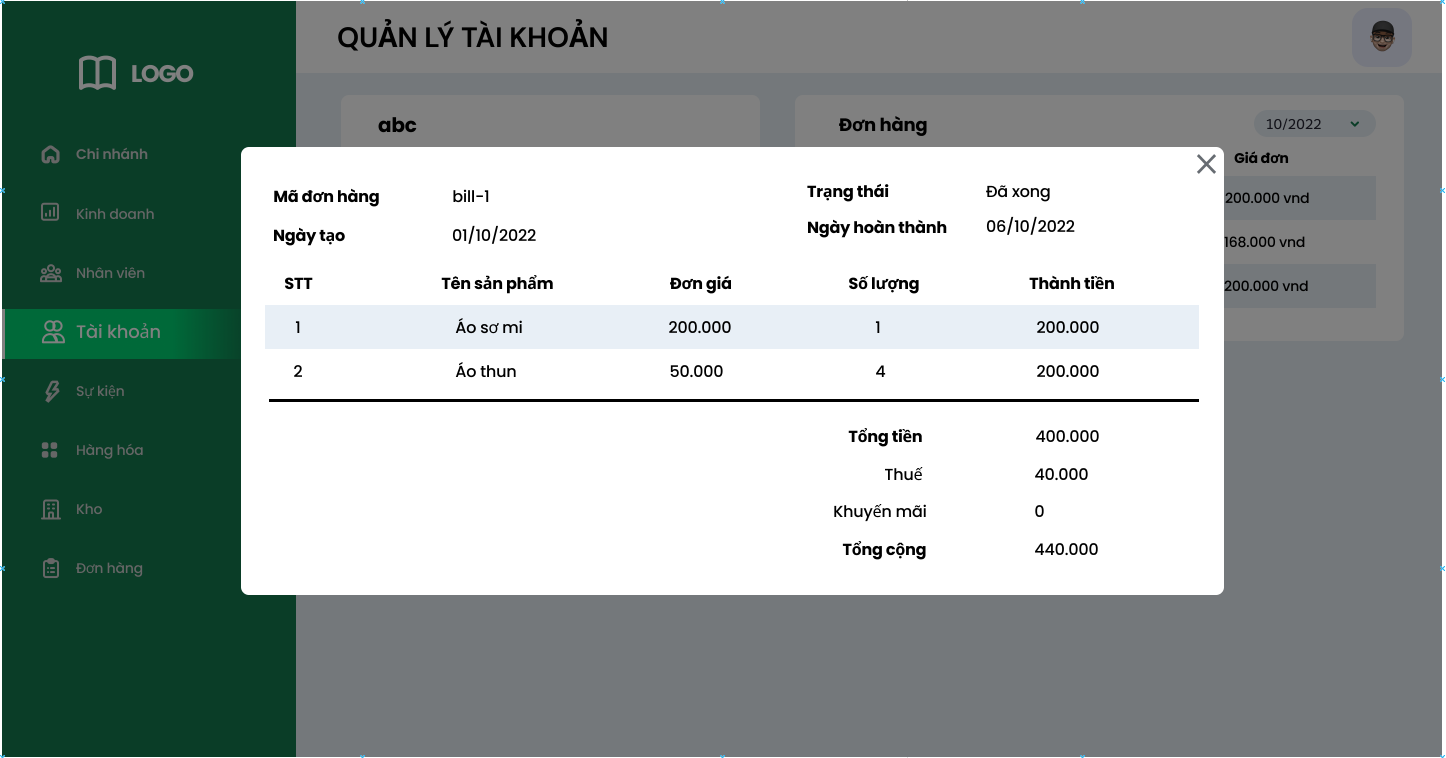
\includegraphics[width=10cm]{img/UI/admin/account_order.png}
                \label{31}
                \newline
                \caption{Giao diện thông tin chi tiết tài khoản}
            \end{figure}
    \subsubsection{Quản lý kho}
        \begin{figure}[!htp]
            \centering
            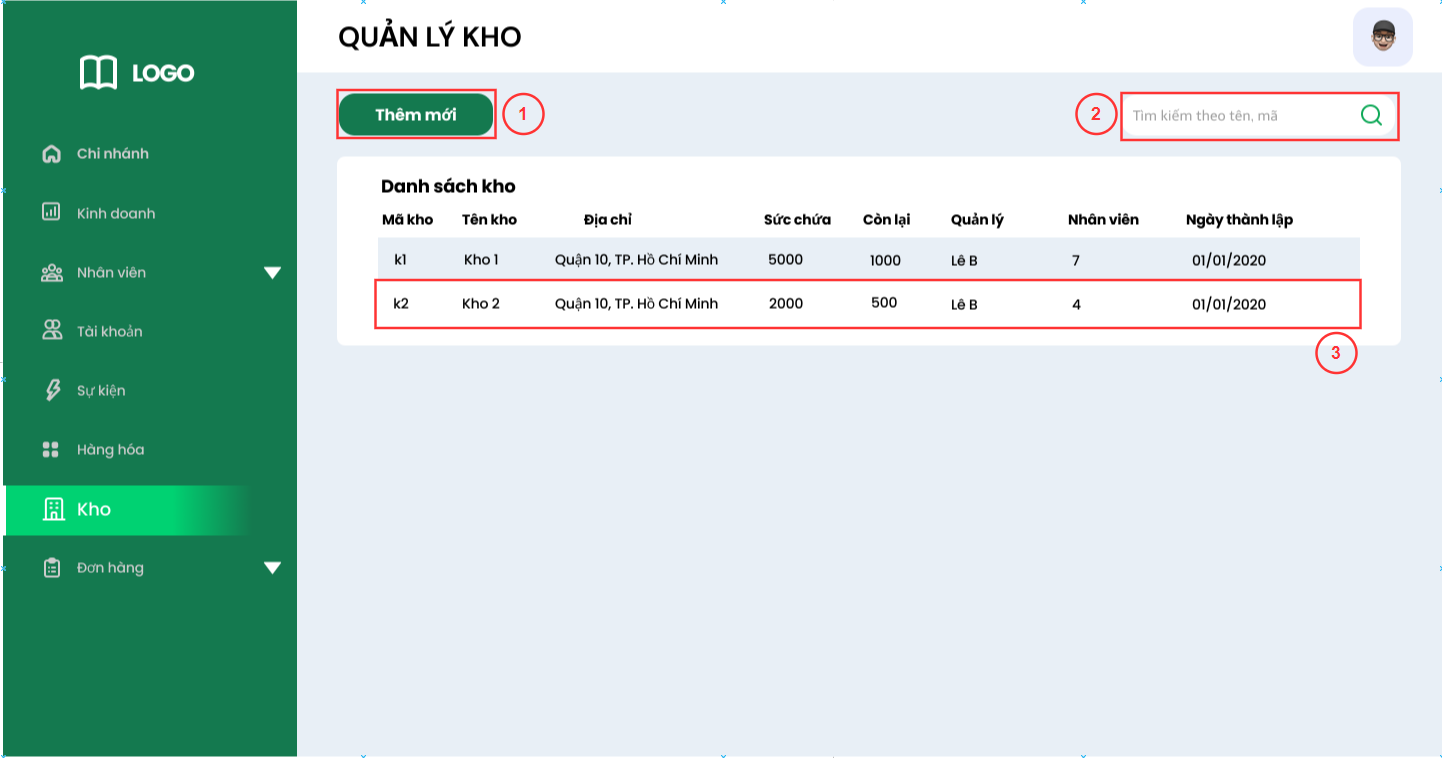
\includegraphics[width=10cm]{img/UI/admin/warehouse.png}
            \label{32}
            \newline
            \caption{Giao diện quản lý kho}
        \end{figure}
        \textbf{Mô tả:}  
        \begin{quote}
            \begin{enumerate}
                \item Chọn để hiện form tạo kho mới
                \item Nhập để tìm kiếm kho theo tên, mã
                \item Chọn để chỉnh sửa thông tin kho
            \end{enumerate}
        \end{quote}
        \subsubsection{Thêm, chỉnh sửa thông tin kho}
            \begin{figure}[!htp]
                \centering
                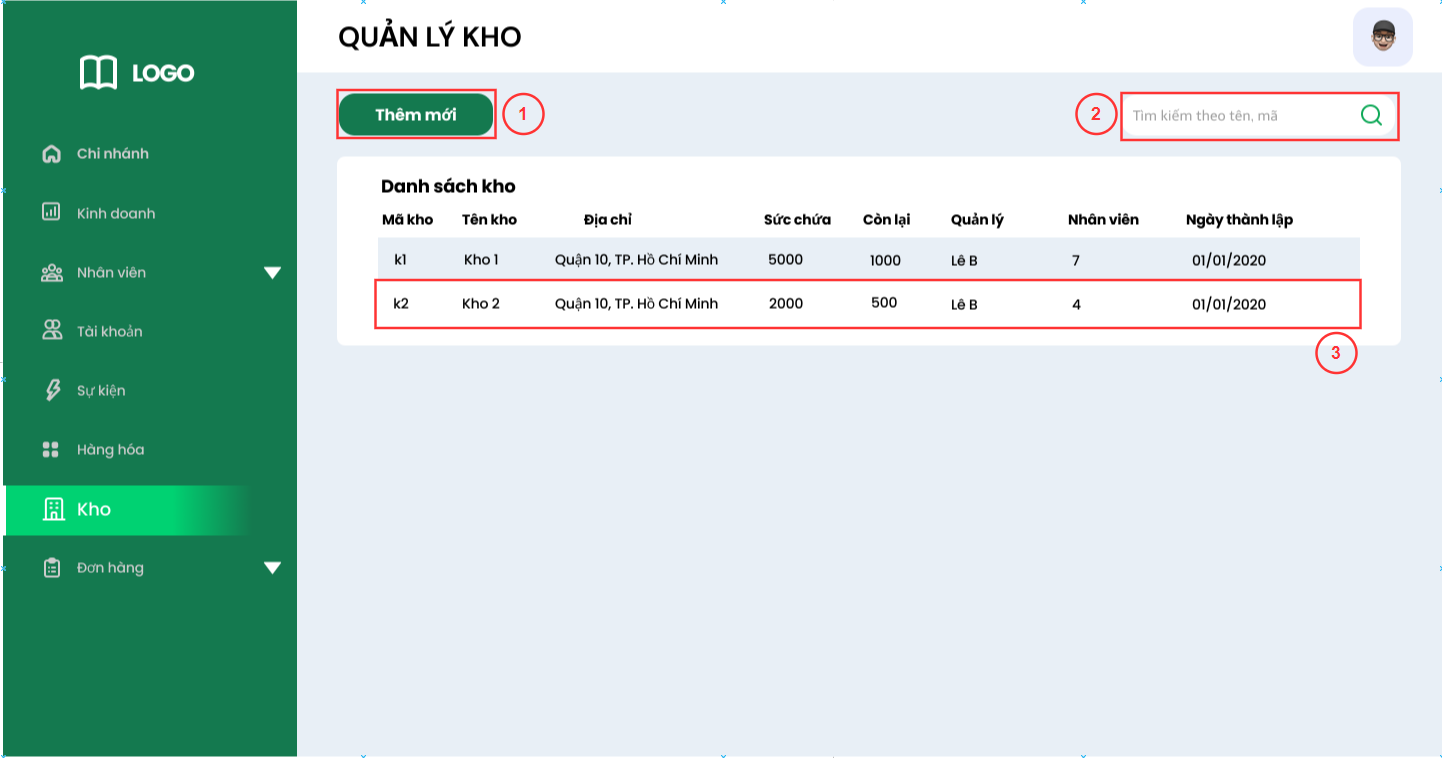
\includegraphics[width=10cm]{img/UI/admin/warehouse.png}
                \label{33}
                \newline
                \caption{Giao diện thêm, chỉnh sửa thông tin kho}
            \end{figure}
            \textbf{Mô tả:}  
            \begin{quote}
                \begin{enumerate}
                    \item Nhập tên kho
                    \item Nhập địa chỉ kho
                    \item Nhập sức chứa kho
                \end{enumerate}
            \end{quote}
    
    \subsubsection{Quản lý sự kiện}
        \begin{figure}[!htp]
            \centering
            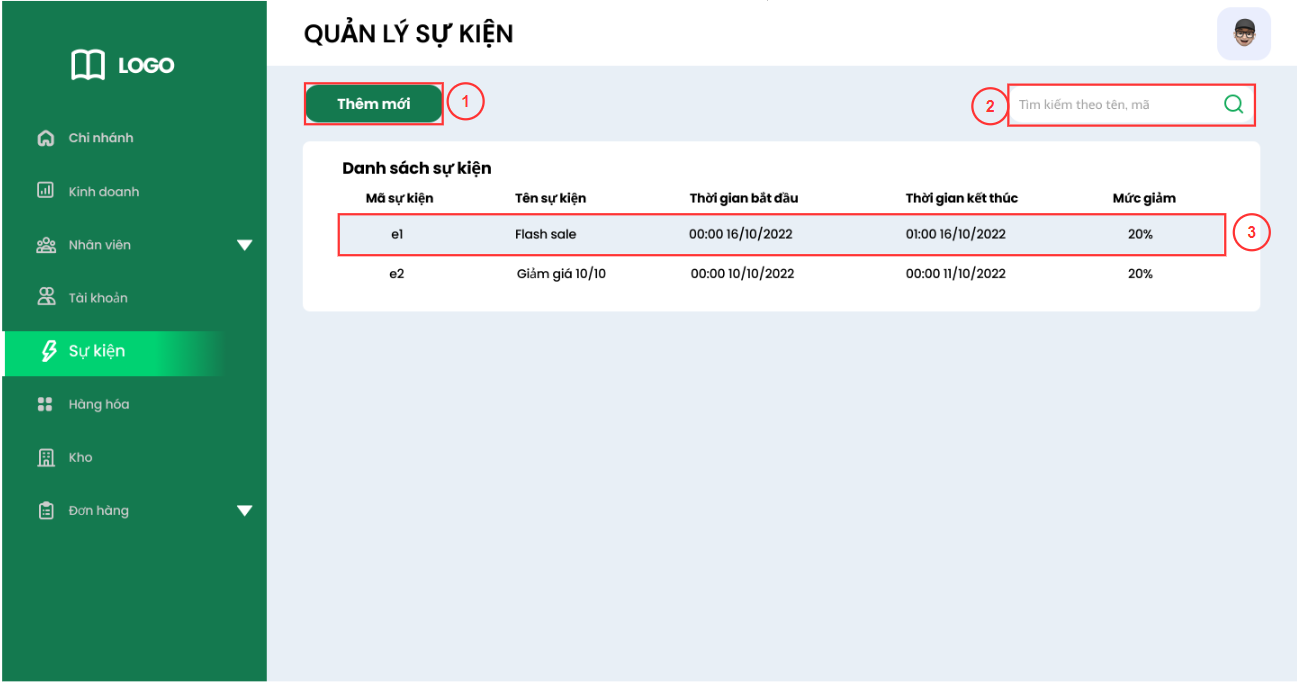
\includegraphics[width=10cm]{img/UI/admin/Event.png}
            \label{34}
            \newline
            \caption{Giao diện quản lý sự kiện}
        \end{figure}
        \textbf{Mô tả:}  
        \begin{quote}
            \begin{enumerate}
                \item Chọn để thêm mới sự kiện
                \item Nhập để tìm kiếm sự kiện theo tên, mã
                \item Chọn để chỉnh sửa thông tin sự kiện
            \end{enumerate}
        \end{quote}
        \subsubsection{Thêm, chỉnh sửa thông tin sự kiện}
            \begin{figure}[!htp]
                \centering
                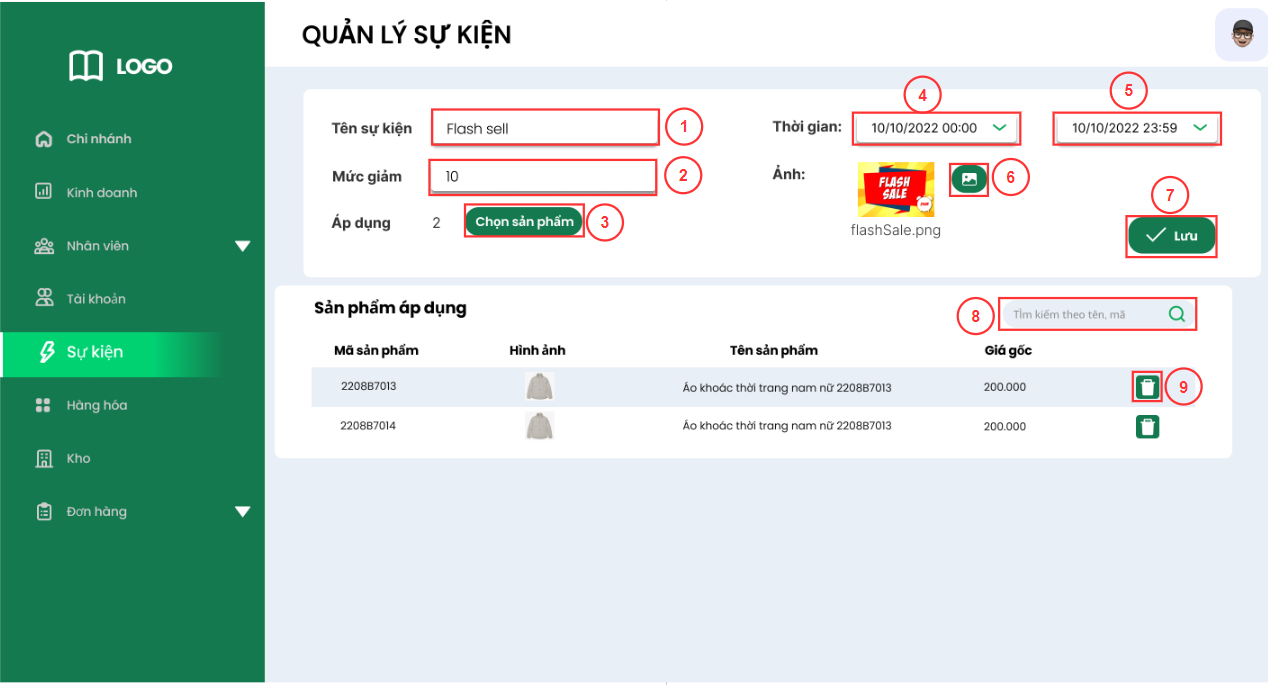
\includegraphics[width=10cm]{img/UI/admin/Event_detail.png}
                \label{35}
                \newline
                \caption{Giao diện thêm, chỉnh sửa thông tin sự kiện}
            \end{figure}
            \textbf{Mô tả:}  
            \begin{quote}
                \begin{enumerate}
                    \item Nhập tên sự kiện
                    \item Nhập mức giảm giá
                    \item Chọn để hiện danh sách sản phẩm
                    \item Chọn thời gian bắt đầu sự kiện
                    \item Chọn thời gian kết thúc sự kiện
                    \item Chọn ảnh cho sự kiện
                    \item Chọn lưu thay đổi thông tin
                    \item Nhập để tìm kiếm các hàng áp dụng sự kiện
                    \item Chọn để xóa hàng khỏi sự kiện
                \end{enumerate}
            \end{quote}
        
        \subsubsection{Chọn hàng cho sự kiện}
            \begin{figure}[!htp]
                \centering
                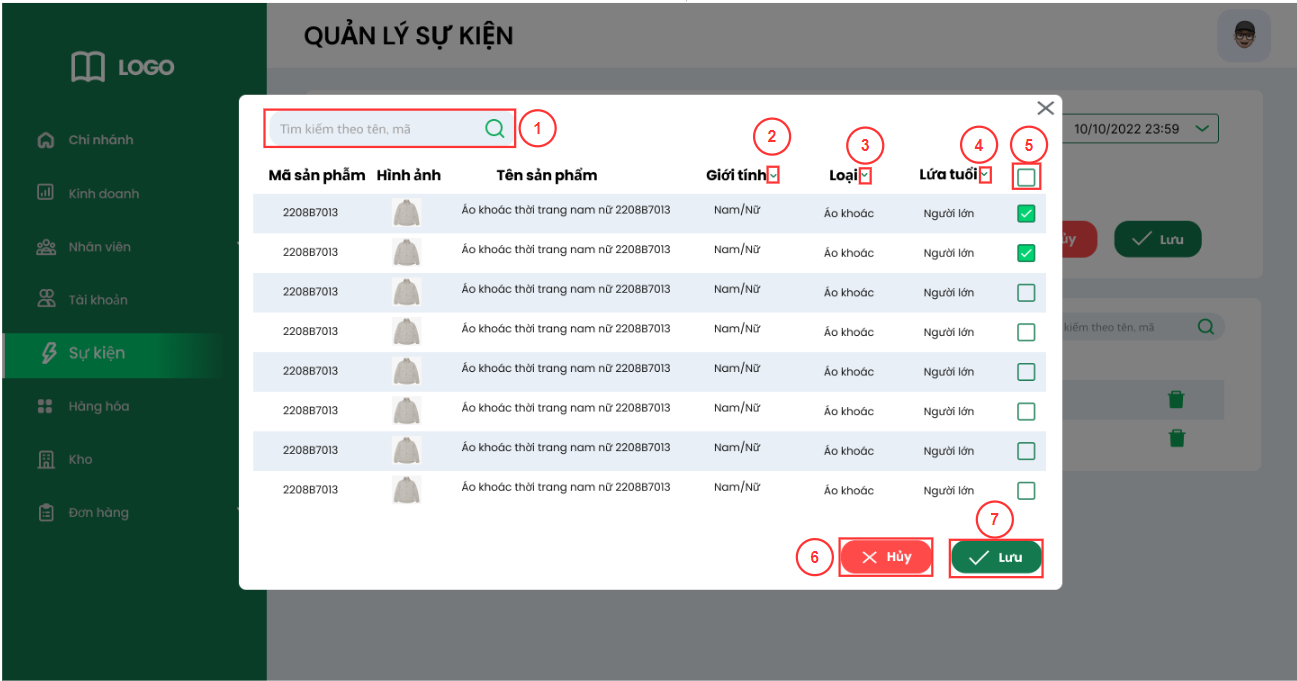
\includegraphics[width=10cm]{img/UI/admin/Event_select.png}
                \label{36}
                \newline
                \caption{Giao diện chọn hàng cho sự kiện}
            \end{figure}
            \textbf{Mô tả:}  
            \begin{quote}
                \begin{enumerate}
                    \item Nhập để tìm kiếm hàng theo tên, mã
                    \item Chọn để lọc hàng theo giới tính
                    \item Chọn để lọc hàng theo loại hàng
                    \item Chọn để lọc hàng theo lứa tuổi
                    \item Đánh dấu để chọn/bỏ chọn hàng
                    \item Chọn để hủy thay đổi
                    \item Chọn để lưu thay đổi
                \end{enumerate}
            \end{quote}
    
    
    \subsubsection{Quản lý hàng hóa}
        \begin{figure}[!htp]
            \centering
            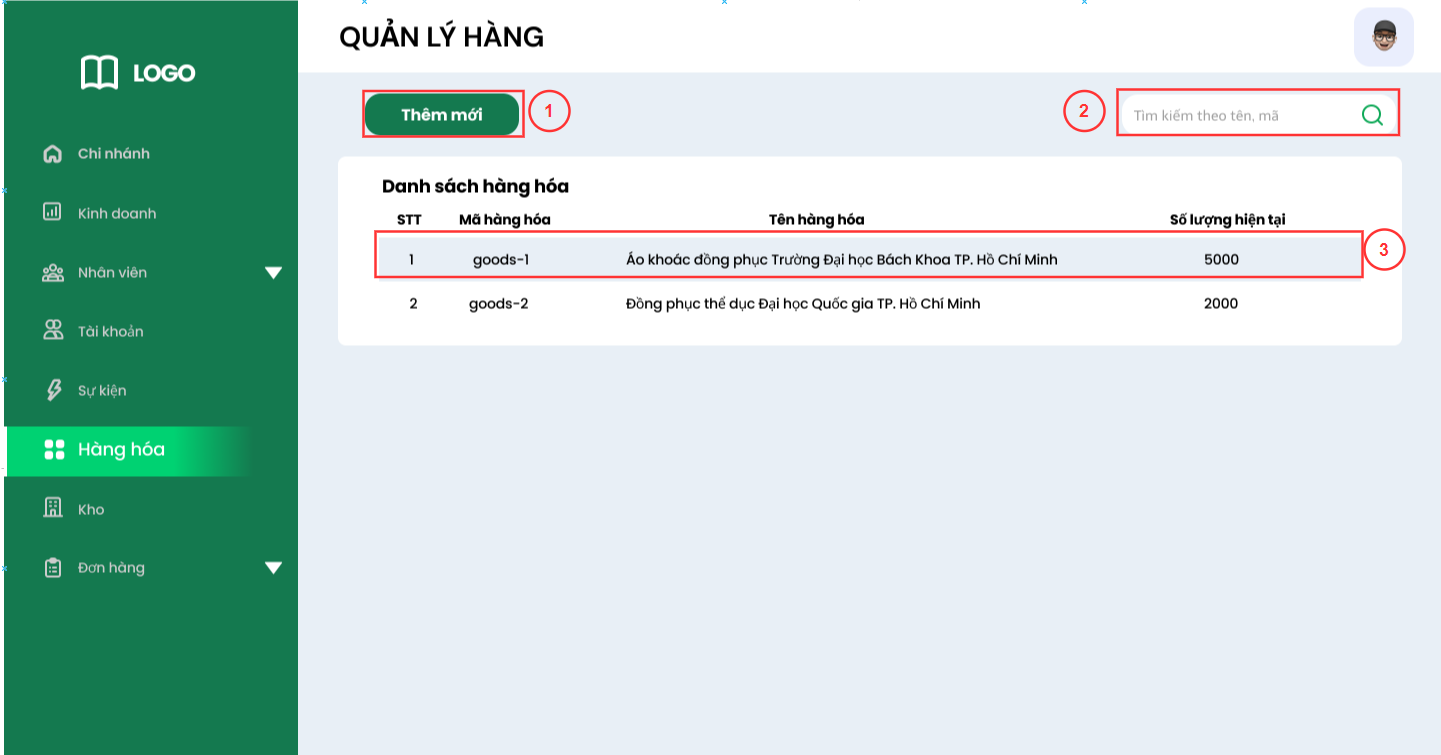
\includegraphics[width=10cm]{img/UI/admin/Goods.png}
            \label{37}
            \newline
            \caption{Giao diện quản lý hàng hóa}
        \end{figure}
        \textbf{Mô tả:}  
        \begin{quote}
            \begin{enumerate}
                \item Chọn thêm hàng hóa
                \item Nhập để tìm kiếm hàng theo tên, mã
                \item Chọn chỉnh sửa thông tin hàng hóa
            \end{enumerate}
        \end{quote}
        
        \subsubsubsection{Chỉnh sửa thông tin hàng}
            \begin{figure}[!htp]
                \centering
                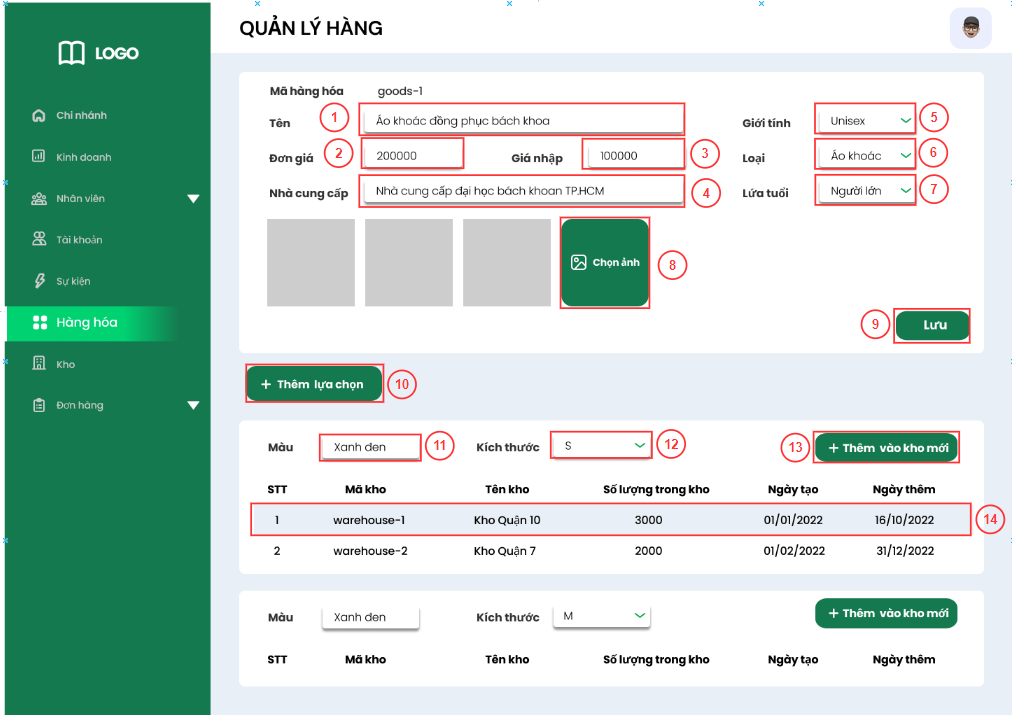
\includegraphics[width=10cm]{img/UI/admin/Goods_edit.png}
                \label{38}
                \newline
                \caption{Giao diện chỉnh sửa thông tin hàng}
            \end{figure}
            \textbf{Mô tả:}  
            \begin{quote}
                \begin{enumerate}
                    \item Nhập tên hàng hóa
                    \item Nhập màu đơn giá hàng hóa
                    \item Nhập giá nhập hàng
                    \item Nhập tên nhà cung cấp
                    \item Chọn giới tính của hàng hóa
                    \item Chọn loại của hàng hóa
                    \item Chọn lứa tuổi của hàng hóa
                    \item Chọn ảnh cho hàng hóa
                    \item Chọn để lưu thay đổi
                    \item Chọn để thêm lựa chọn về màu sắc, kích thước
                    \item Chọn để đổi màu sản phẩm
                    \item Chọn kích thước sản phẩm
                    \item Chọn để thêm sp vào kho ms
                    \item Chọn để vận chuyển hàng trong kho
                \end{enumerate}
            \end{quote}
            
        \subsubsubsection{Vận chuyển hàng}
            \begin{figure}[!htp]
                \centering
                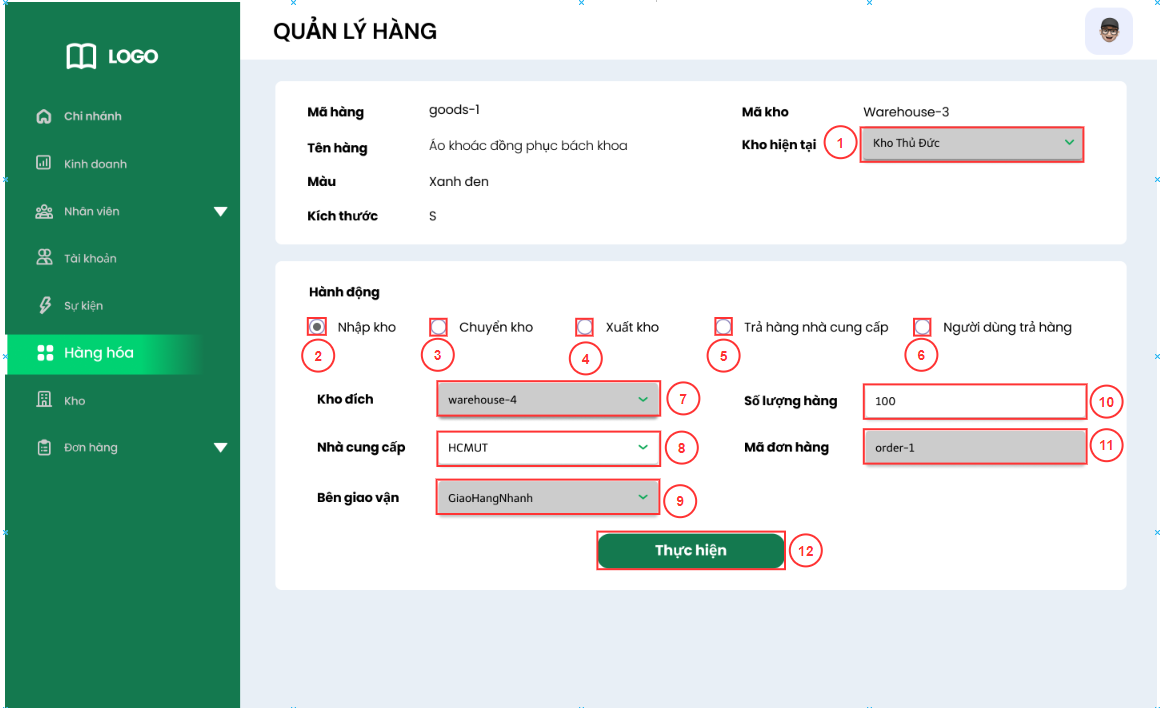
\includegraphics[width=10cm]{img/UI/admin/Goods_tranfer.png}
                \label{39}
                \newline
                \caption{Giao diện vận chuyển hàng}
            \end{figure}
            \textbf{Mô tả:}  
            \begin{quote}
                \begin{enumerate}
                    \item Chọn kho khi nhập kho mới
                    \item Chọn để thực hiện nhập kho
                    \item Chọn để thực hiện chuyển kho
                    \item Chọn để thực hiện xuất kho
                    \item Chọn để thực hiện trả hàng cho nhà cung cấp kho
                    \item Chọn để thực hiện nhận hàng trả
                    \item Chọn kho đích đến để chuyển hàng
                    \item Chọn nhà cung cấp khi nhập kho
                    \item Chọn bên giao vận khi chuyển kho, xuất kho
                    \item Nhập số lượng hàng để thực hiện các hoạt động
                    \item Nhập mã đơn để xuất kho, nhận trả hàng
                    \item Chọn để thực hiện hành động
                \end{enumerate}
            \end{quote}
        
        
        
    \subsubsection{Quản lý đơn hàng trực tuyến}
    \begin{figure}[!htp]
        \centering
        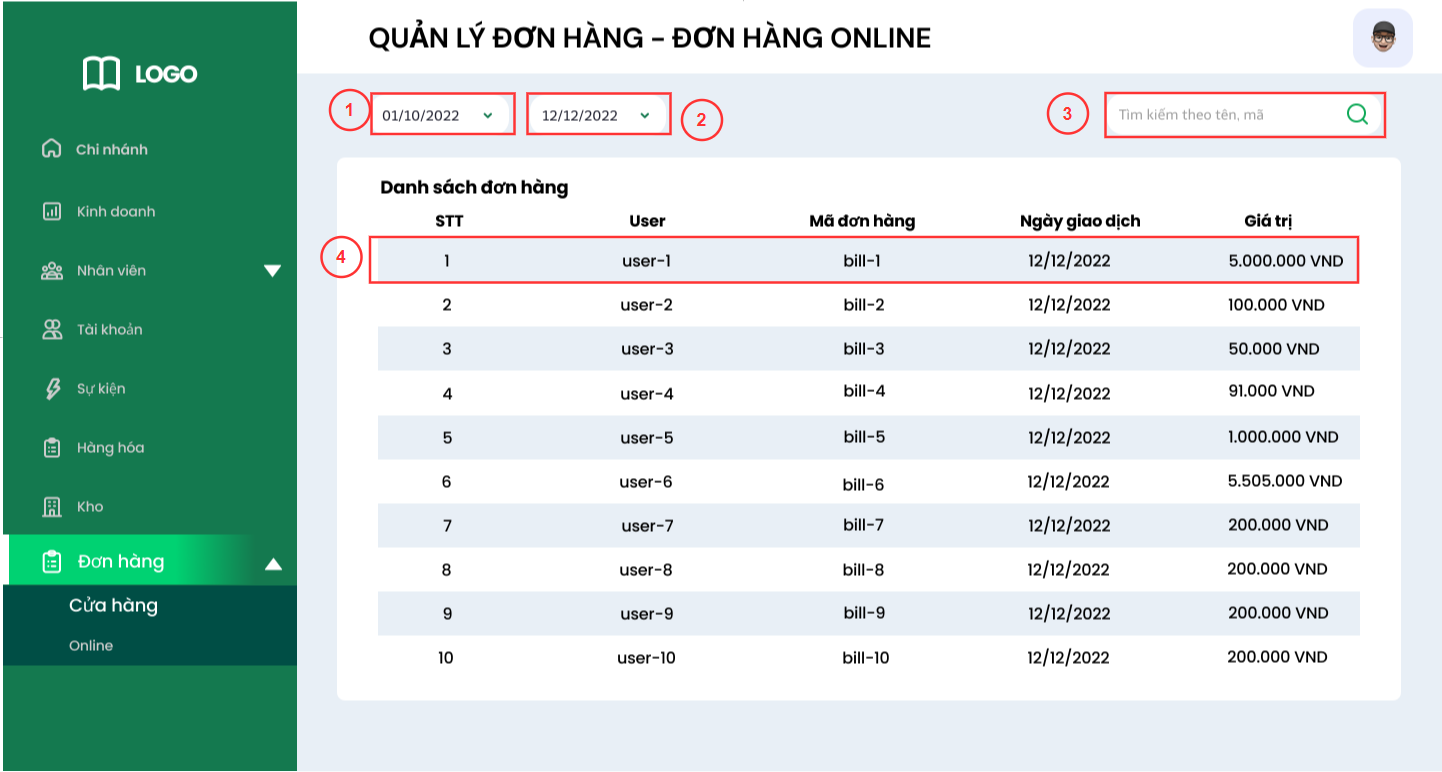
\includegraphics[width=3.8in]{img/UI/admin/OnlineOrder.png}
        \label{40}
        \newline
        \caption{Giao diện quản lý đơn hàng trực tuyến}
    \end{figure}
    \textbf{Mô tả:}  
    \begin{quote}
        \begin{enumerate}
            \item Chọn thời gian bắt đầu
            \item Chọn thời gian kết thúc
            \item Nhập để lọc đơn theo mã đơn
            \item Chọn để xem chi tiết đơn hàng
        \end{enumerate}
    \end{quote}
    
        \subsubsubsection{Chi tiết đơn hàng trực tuyến}
        \begin{figure}[!htp]
            \centering
            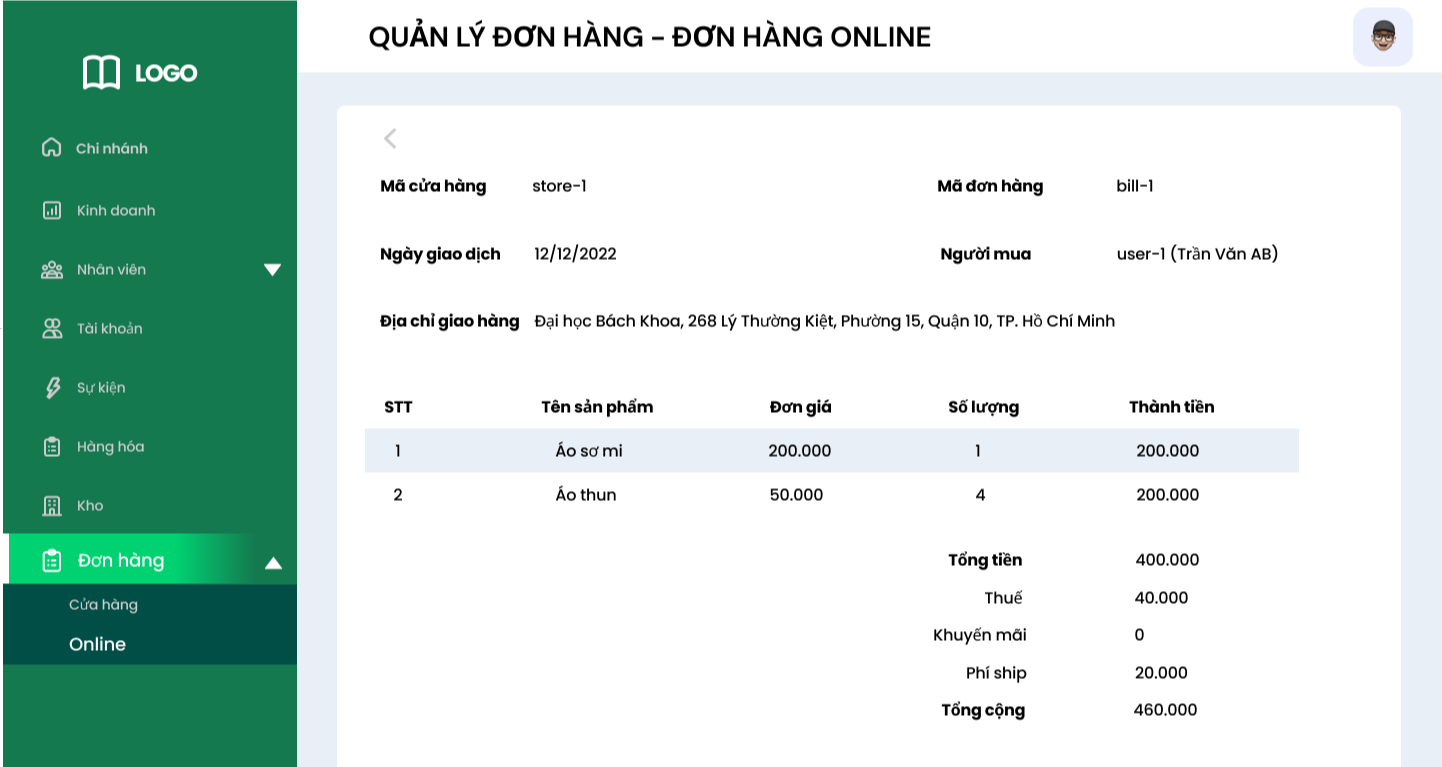
\includegraphics[width=3.8in]{img/UI/admin/OnlineOrder_detail.png}
            \label{41}
            \newline
            \caption{Giao diện chi tiết đơn hàng trực tuyến}
        \end{figure}
    
    
    
    \subsubsection{Quản lý đơn hàng trực tiếp}
    \begin{figure}[!htp]
        \centering
        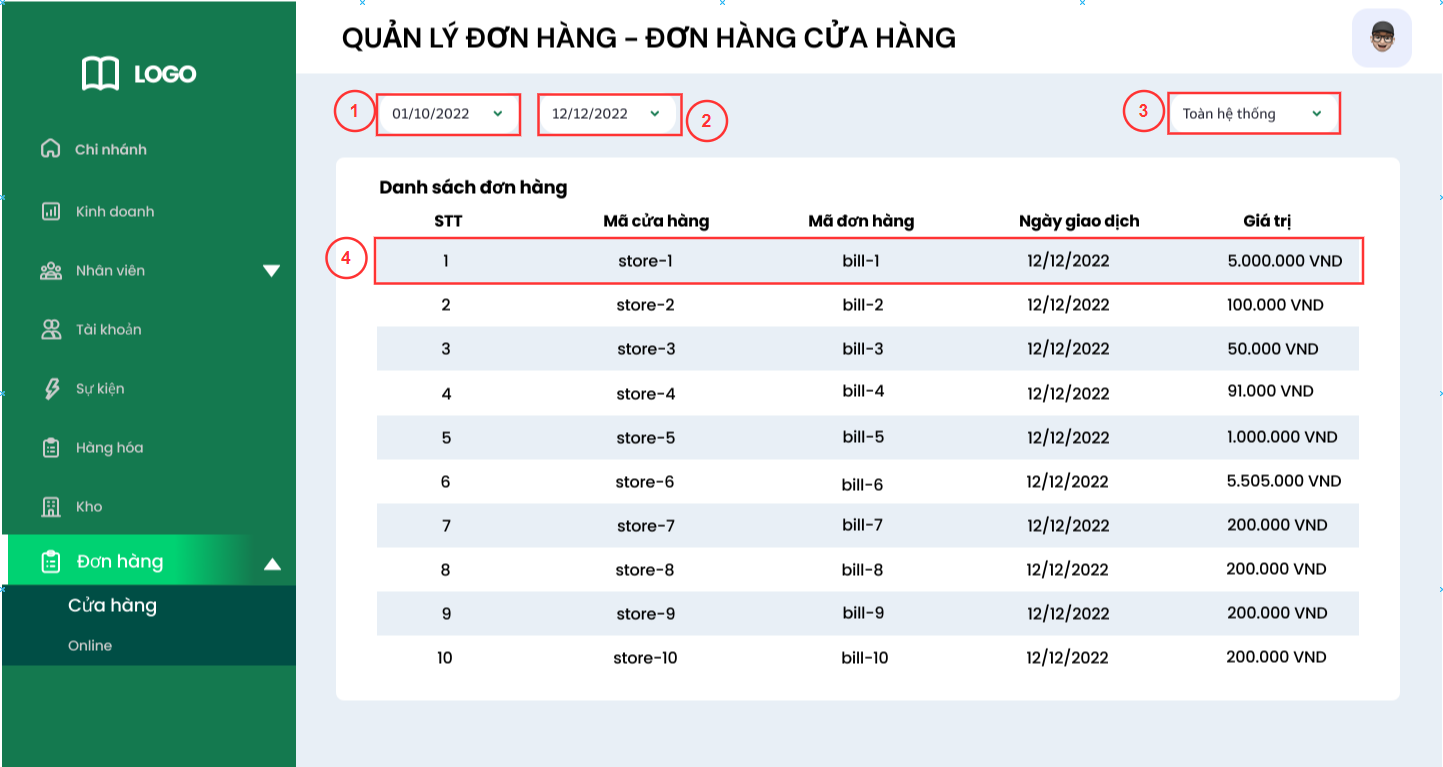
\includegraphics[width=3.8in]{img/UI/admin/OfflineOrder.png}
        \label{42}
        \newline
        \caption{Giao diện quản lý đơn hàng cửa hàng}
    \end{figure}
    \textbf{Mô tả:}  
    \begin{quote}
        \begin{enumerate}
            \item Chọn thời gian bắt đầu
            \item Chọn thời gian kết thúc
            \item Nhập để lọc đơn theo mã đơn
            \item Chọn để xem chi tiết đơn hàng
        \end{enumerate}
    \end{quote}
        \subsubsubsection{Chi tiết đơn hàng cửa hàng}
        \begin{figure}[!htp]
            \centering
            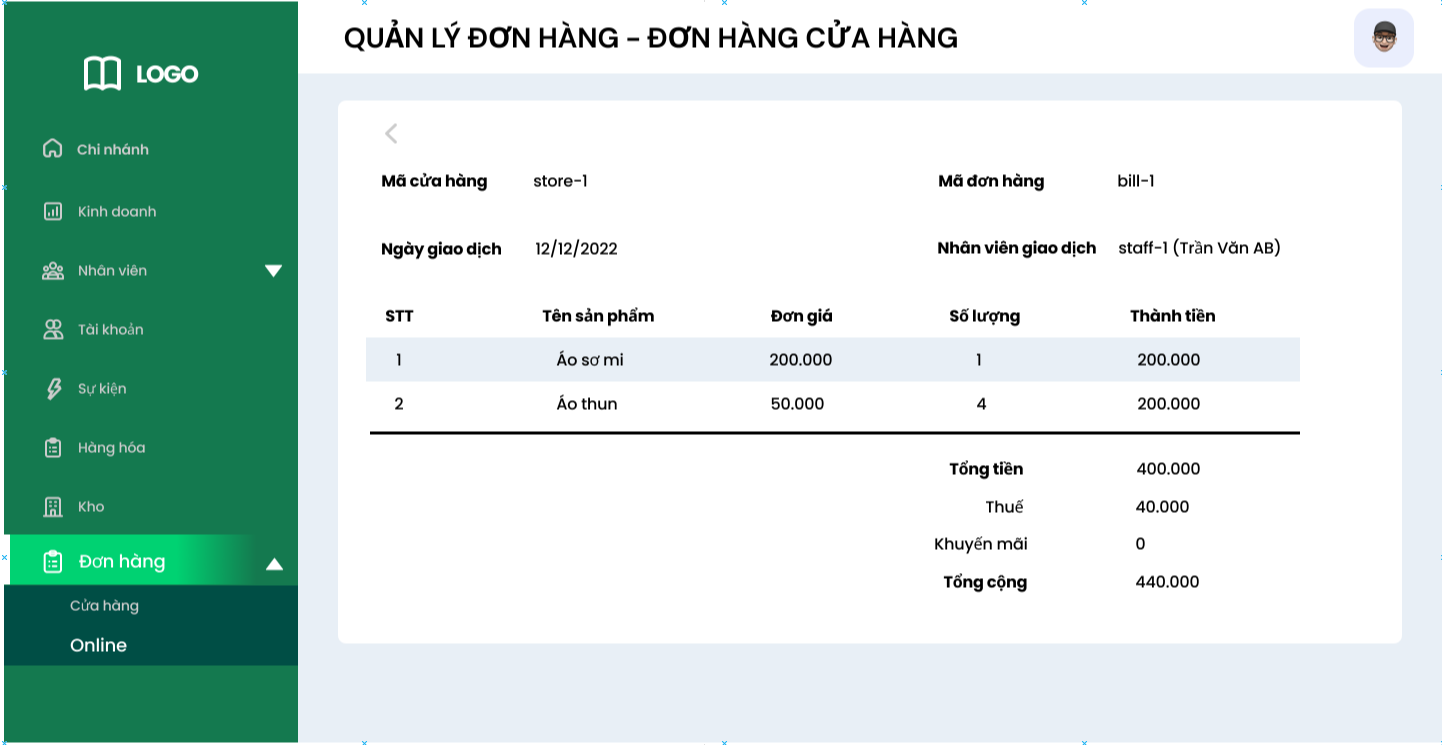
\includegraphics[width=3.8in]{img/UI/admin/OfflineOrder_detai;.png}
            \label{43}
            \newline
            \caption{Giao diện chi tiết đơn hàng cửa hàng}
        \end{figure}


    \subsubsection{Giao diện khác}
        Bên cạnh quản trị viên, quản lý ở cấp cao nhất thì còn các quản lý ở từng mảng và chỉ sử dụng được một vài chức năng của quản trị viên nên chỉ có sự khác nhau về phần sidebar:
        \begin{itemize}
            \item Quản lý chi nhánh: Quản lý chi nhánh, quản lý hoạt động kinh doanh, quản lý nhân viên, quản lý đơn hàng cửa hàng
            \item Trưởng chi nhánh: Quản lý hoạt động kinh doanh (riêng chi nhánh), quản lý nhân viên(riêng chi nhánh), quản lý đơn hàng(riêng chi nhánh).
            \item Quản lý hàng hóa: Quản lý hàng hóa
            \item Quản lý kho: Quản lý kho, quản lý nhân viên kho
        \end{itemize}
        \subsubsubsection{Quản lý chi nhánh}
            \begin{figure}[!htp]
                \centering
                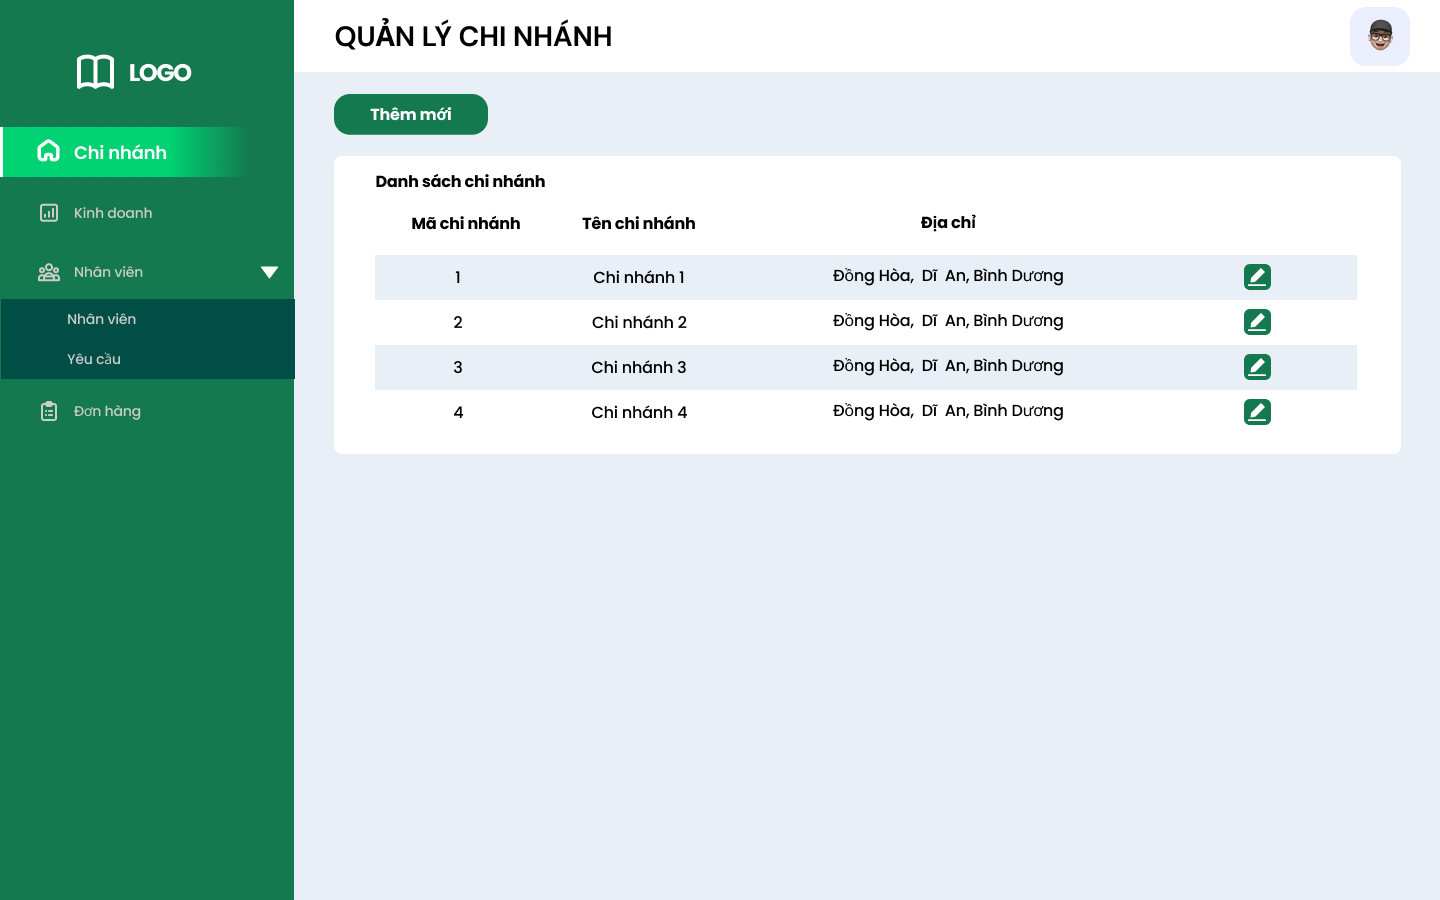
\includegraphics[width=3.8in]{img/UI/admin/sub-admin. Quản lý chi nhánh.png}
                \label{44}
                \newline
                \caption{Giao diện của người quản lý chi nhánh}
            \end{figure}
        
        \subsubsubsection{Trưởng chi nhánh}
            \begin{figure}[!htp]
                \centering
                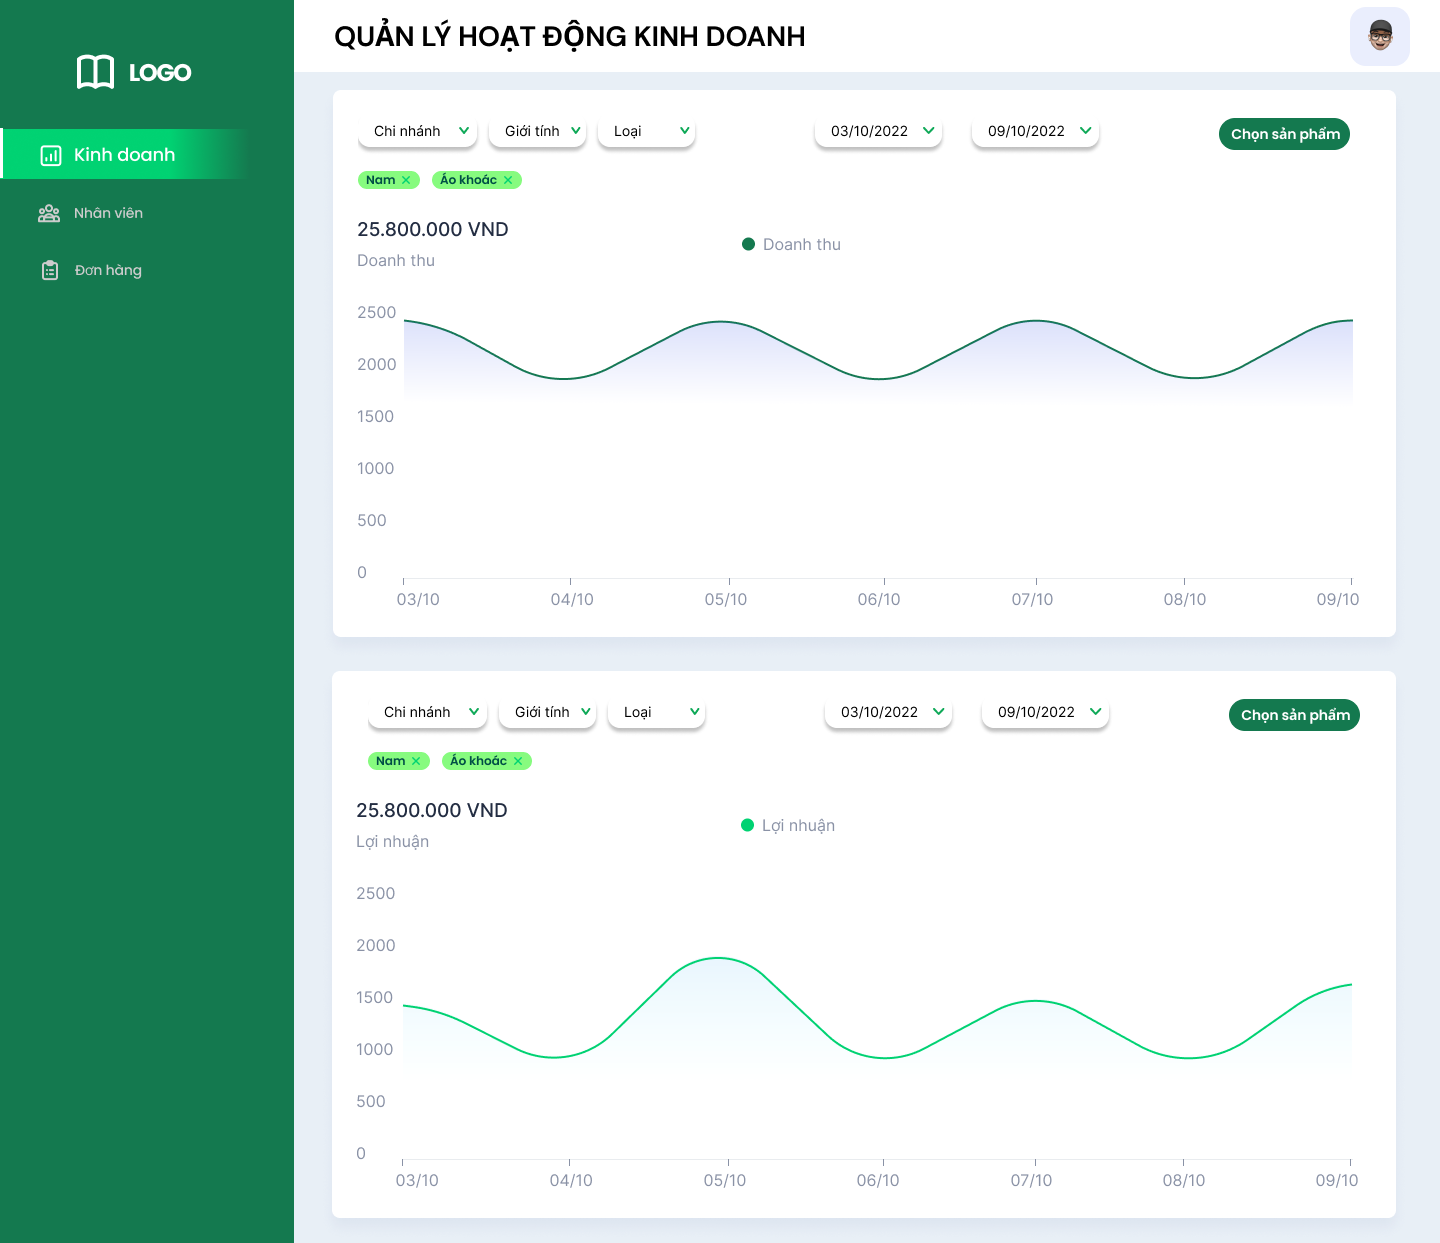
\includegraphics[width=3.8in]{img/UI/admin/branch-leader.png}
                \label{45}
                \newline
                \caption{Giao diện của người trưởng chi nhánh}
            \end{figure}
        
        \subsubsubsection{Quản lý hàng hóa}
            \begin{figure}[!htp]
                \centering
                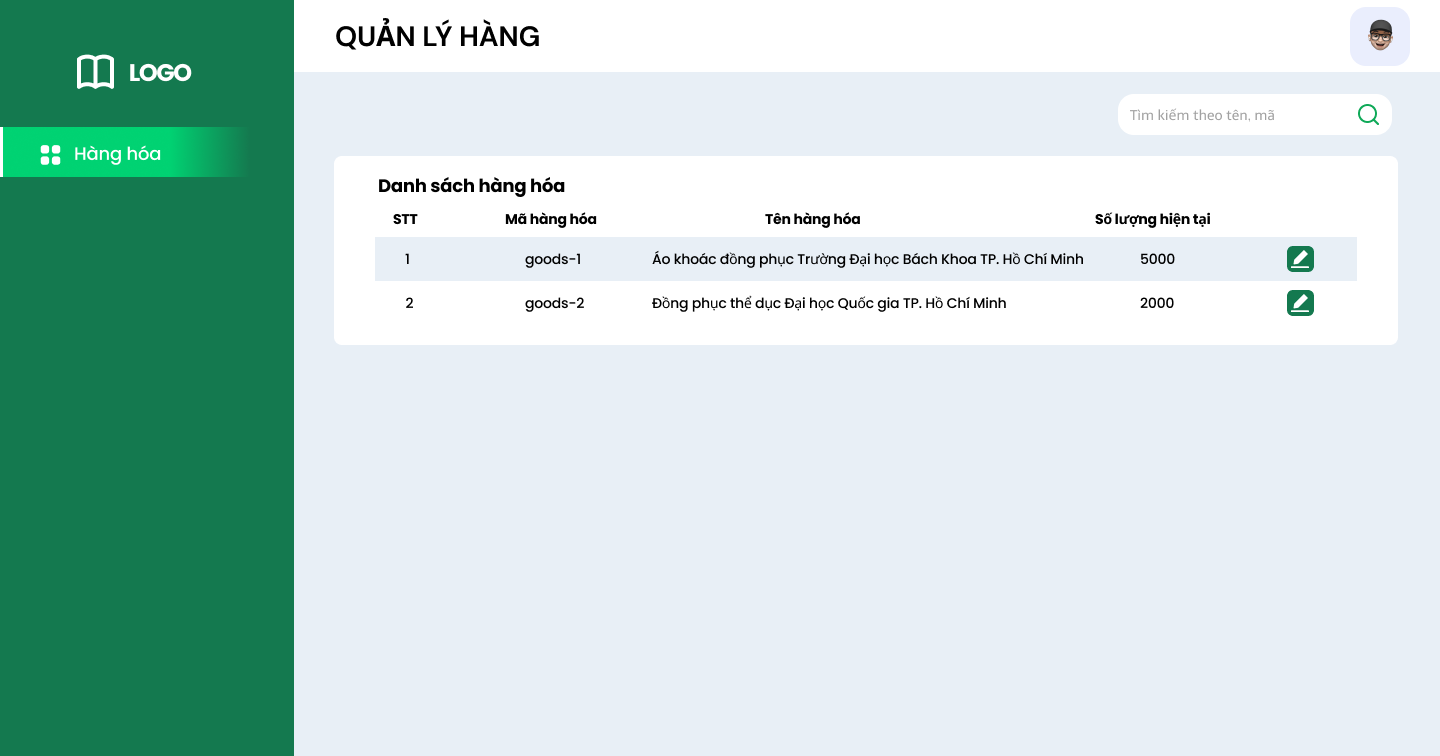
\includegraphics[width=3.8in]{img/UI/admin/sub ADmin -Quản lý hàng.png}
                \label{46}
                \newline
                \caption{Giao diện của người quản lý hàng hóa}
            \end{figure}
        
        \subsubsubsection{Quản lý kho}
            \begin{figure}[!htp]
                \centering
                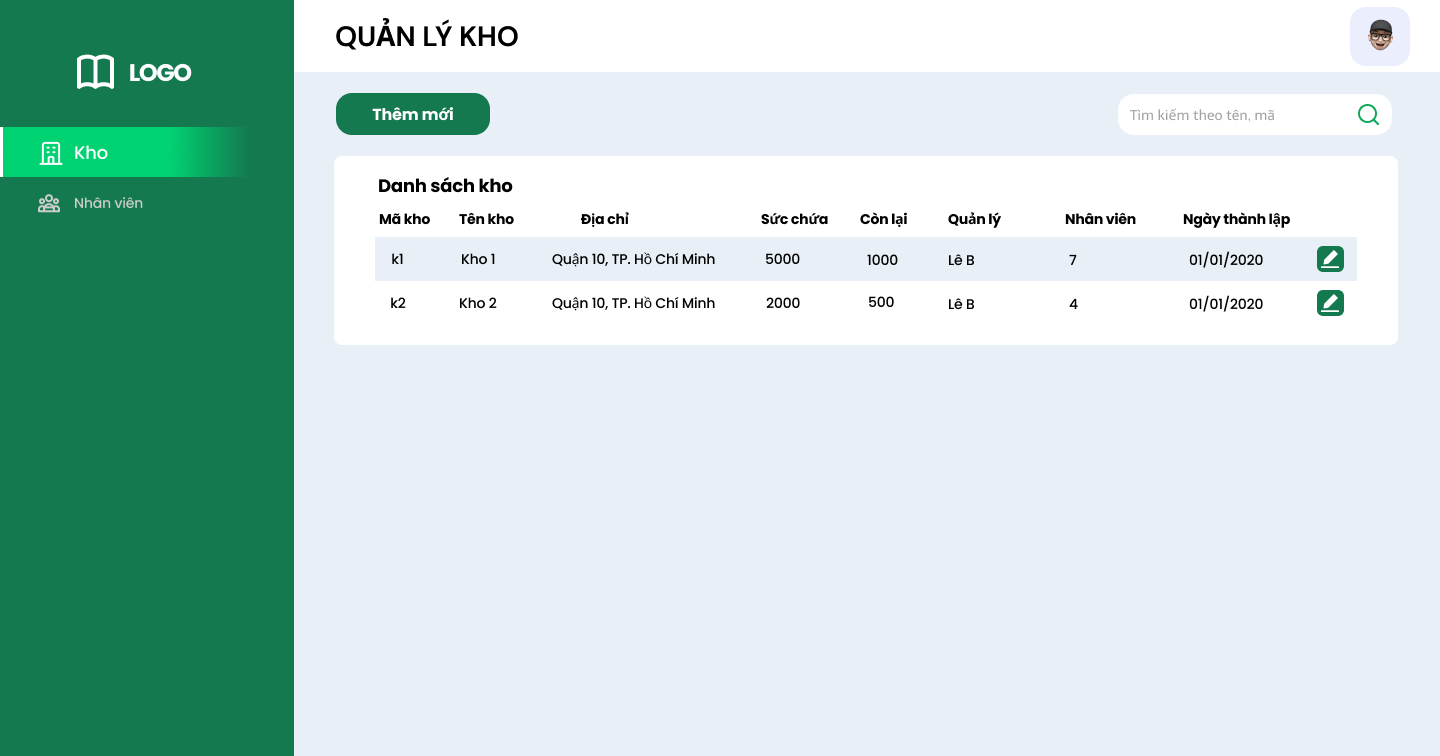
\includegraphics[width=3.8in]{img/UI/admin/sub-admin -Quản lý kho.png}
                \label{47}
                \newline
                \caption{Giao diện của người quản lý kho }
            \end{figure}
    
    